\documentclass[a4paper]{report}
\usepackage[utf8]{vietnam}
\usepackage[utf8]{inputenc}
\usepackage{amsmath}
\usepackage{amsfonts}
\usepackage{amssymb}
\usepackage{graphicx}
\usepackage{xspace}
% \usepackage{caption}
\usepackage[font=small]{caption}
\usepackage{booktabs}
\usepackage[unicode]{hyperref}
\usepackage[left=3cm,right=2cm,top=2.5cm,bottom=3cm]{geometry}
\usepackage{titlesec} 
\usepackage{scrextend}
\usepackage{enumerate}
\usepackage{url}
\usepackage{tikz}
\usepackage{float}
\usepackage{afterpage}
\usepackage{multirow}
\usepackage{sectsty}
\usepackage{tocloft,calc}
\usepackage{listings}
\usepackage{makecell}
\usepackage[sort&compress]{natbib}
\usetikzlibrary{calc}
\usepackage{algorithm}
\usepackage{subcaption}
% \usepackage{minted}
% \usepackage[perpage]{footmisc}
\usepackage[flushleft]{threeparttable}
% \usepackage{subcaption}
\usepackage{perpage} %the perpage package
\usepackage{tabularx}
\usepackage{ragged2e}
\MakePerPage{footnote} %the perpage package command
% \usepackage[ruled,vlined]{algorithm2e}
\PassOptionsToPackage{table}{xcolor}

\def\changemargin#1#2{\list{}{\rightmargin#2\leftmargin#1}\item[]}
\let\endchangemargin=\endlist 

\changefontsizes{13pt}
\bibliographystyle{unsrt}

\makeatletter
\def\l@figure{\@dottedtocline{1}{1em}{2.2em}}
\def\l@table{\@dottedtocline{1}{1em}{2.2em}}
\renewcommand*{\ALG@name}{Thuật toán}
\makeatother

\sectionfont{\fontsize{15}{15}\selectfont}
\subsectionfont{\fontsize{13}{15}\selectfont}

\titleformat{\chapter}[display]   
{\normalfont\huge\bfseries}{\chaptertitlename\ \thechapter}{0pt}{\LARGE}
\titlespacing*{\chapter}{0cm}{-\topskip}{0pt}[0pt]

\renewcommand{\baselinestretch}{1.3}
%\renewcommand{\cftsecpresnum}{Chương\space}
\renewcommand{\cftchappresnum}{Chương }
\AtBeginDocument{\addtolength\cftchapnumwidth{\widthof{\bfseries Chương }}}
\setlength{\parskip}{0.4em}
\setlength{\parindent}{0pt}
%
\title{Xây dựng ứng dụng quản lý nhóm chat sự kiện tích hợp AI tạo video}	%% title
\author{Nguyễn Thành Dũng}			%% author's name
%
\newcommand{\argmax}{\arg\!\max}
\newcommand{\tool}{\textsc{DeFP}\xspace}
\newcommand{\toolLong}{\textbf{De}tect \textbf{F}alse \textbf{P}ositive\xspace}

\definecolor{dkgreen}{rgb}{0,0.6,0}
\definecolor{gray}{rgb}{0.5,0.5,0.5}
\definecolor{mauve}{rgb}{0.58,0,0.82}
\definecolor{gray}{rgb}{0.4,0.4,0.4}
\definecolor{darkblue}{rgb}{0.0,0.0,0.6}
\definecolor{lightblue}{rgb}{0.0,0.0,0.9}
\definecolor{cyan}{rgb}{0.0,0.6,0.6}
\definecolor{darkred}{rgb}{0.6,0.0,0.0}
\definecolor{bg_gray}{RGB}{242, 242, 235}

\renewcommand{\lstlistingname}{Hình}
\newcommand{\cev}[1]{\reflectbox{\ensuremath{\vec{\reflectbox{\ensuremath{#1}}}}}}

\setlength{\cftsubsecnumwidth}{3.2em}

\lstset{
  basicstyle=\ttfamily\footnotesize,
  columns=fullflexible,
  showstringspaces=false,
  numbers=left,                   % where to put the line-numbers
  numberstyle=\small\color{gray},  % the style that is used for the line-numbers
  stepnumber=1,
  numbersep=5pt,                  % how far the line-numbers are from the code
  backgroundcolor=\color{bg_gray},      % choose the background color. You must add \usepackage{color}
  showspaces=false,               % show spaces adding particular underscores
  showstringspaces=false,         % underline spaces within strings
  showtabs=false,                 % show tabs within strings adding particular underscores
  frame=none,                   % adds a frame around the code
  rulecolor=\color{black},        % if not set, the frame-color may be changed on line-breaks within not-black text (e.g. commens (green here))
  tabsize=2,                      % sets default tabsize to 2 spaces
  captionpos=b,                   % sets the caption-position to bottom
  breaklines=true,                % sets automatic line breaking
  breakatwhitespace=false,        % sets if automatic breaks should only happen at whitespace
  title=\lstname,                   % show the filename of files included with \lstinputlisting;
                                  % also try caption instead of title  
  commentstyle=\color{gray}\upshape
}


\lstdefinelanguage{XML}
{
  morestring=[s][\color{mauve}]{"}{"},
  morestring=[s][\color{black}]{>}{<},
  morecomment=[s]{<?}{?>},
  morecomment=[s][\color{dkgreen}]{<!--}{-->},
  stringstyle=\color{black},
  identifierstyle=\color{lightblue},
  keywordstyle=\color{red},
  morekeywords={xmlns,xsi,noNamespaceSchemaLocation,type,id,x,y,source,target,version,tool,transRef,roleRef,objective,eventually}% list your attributes here
}

\definecolor{codegreen}{rgb}{0,0.6,0}
\definecolor{codegray}{rgb}{0.5,0.5,0.5}
\definecolor{codepurple}{rgb}{0.58,0,0.82}
\definecolor{backcolour}{rgb}{0.95,0.95,0.92}

\begin{document}
% Cover Vietnamese 1

% Cover Vietnamese 1

\pagenumbering{gobble}
\begin{center}
	
\begin{tikzpicture}[overlay,remember picture]
	    \draw [line width=3pt,rounded corners=0pt,
	        ]
	        ($ (current page.north west) + (25mm,-25mm) $)
	        rectangle
	        ($ (current page.south east) + (-15mm,25mm) $);
	    \draw [line width=1pt,rounded corners=0pt]
	        ($ (current page.north west) + (26.5mm,-26.5mm) $)
	        rectangle
	        ($ (current page.south east) + (-16.5mm,26.5mm) $);
	\end{tikzpicture}
	\\[1mm]
	%%12pt
	\textbf{ĐẠI HỌC QUỐC GIA HÀ NỘI\\TRƯỜNG ĐẠI HỌC CÔNG NGHỆ}\\[1cm]
	
\includegraphics[width=0.2\linewidth]{figures/uet}\\[0.3cm]
	\textbf{Nguyễn Thành Dũng}
	\\[2cm]
	
	\large{\textbf{XÂY DỰNG ỨNG DỤNG QUẢN LÝ THƯ VIỆN ẢNH TÍCH HỢP AI TẠO VIDEO}}
	\\[2.6cm]
	\normalsize{\textbf{KHOÁ LUẬN TỐT NGHIỆP ĐẠI HỌC
		\\[2mm]
	Ngành: Công nghệ thông tin}}

	\vfill
	\textbf{HÀ NỘI - 2025}\vspace{10mm}
\end{center}

\begin{center}
	
	
\begin{tikzpicture}[overlay,remember picture]
	\draw [line width=3pt,rounded corners=0pt,
	]
	($ (current page.north west) + (25mm,-25mm) $)
	rectangle
	($ (current page.south east) + (-15mm,25mm) $);
	\draw [line width=1pt,rounded corners=0pt]
	($ (current page.north west) + (26.5mm,-26.5mm) $)
	rectangle
	($ (current page.south east) + (-16.5mm,26.5mm) $);
	\end{tikzpicture}
	\\[1mm]
	\textbf{ĐẠI HỌC QUỐC GIA HÀ NỘI\\TRƯỜNG ĐẠI HỌC CÔNG NGHỆ}
	\\[1cm]
	
\includegraphics[width=0.2\linewidth]{figures/uet}
	\\[0.3cm]
	\textbf{Nguyễn Thành Dũng}
	\\[2cm]
	
	\large{\textbf{XÂY DỰNG ỨNG DỤNG QUẢN LÝ THƯ VIỆN ẢNH TÍCH HỢP AI TẠO VIDEO}}
	\\[2.6cm]
	\normalsize{\textbf{KHOÁ LUẬN TỐT NGHIỆP ĐẠI HỌC
		\\[2mm]
	Ngành: Công nghệ thông tin}}
\end{center}
\vspace{16mm}
\hspace*{12mm}\textbf{ Cán bộ hướng dẫn: TS. Lê Khánh Trình}\\[0.8cm]
\hspace*{12mm}\textbf{ Cán bộ đồng hướng dẫn: TS. Đặng Trần Bình}
\vfill
\begin{center}
	\textbf{HÀ NỘI - 2025}\vspace{10mm}
\end{center}

% NOTE: Cover English 

% \begin{center}
	
% 	\begin{tikzpicture}[overlay,remember picture]
% 	\draw [line width=3pt,rounded corners=0pt,
% 	]
% 	($ (current page.north west) + (25mm,-25mm) $)
% 	rectangle
% 	($ (current page.south east) + (-15mm,25mm) $);
% 	\draw [line width=1pt,rounded corners=0pt]
% 	($ (current page.north west) + (26.5mm,-26.5mm) $)
% 	rectangle
% 	($ (current page.south east) + (-16.5mm,26.5mm) $);
% 	\end{tikzpicture}
% 	\\[1mm]
% 	\textbf{ VIETNAM NATIONAL UNIVERSITY, HANOI\\UNIVERSITY OF ENGINEERING AND TECHNOLOGY}
% 	\\[1cm]
% 	
\includegraphics[width=0.2\linewidth]{figures/uet}
% 	\\[0.3cm]
% 	\textbf{Nguyen Van A}
% 	\\[2cm]
	
% 	\textbf{THESIS TITLE}
% 	\\[2.6cm]
% 	\textbf{BACHELOR'S THESIS
% 		\\[2mm]
% 		Major: Information technology}
% \end{center}
% \vspace{16mm}
% \hspace*{12mm}\textbf{ Supervisor: Dr. ...}\\[0.8cm]
% \hspace*{12mm}\textbf{ Co-Supervisor: Dr. ...}
% \vfill
% \begin{center}
% 	\textbf{HANOI - 2022}
% 	\vspace{4mm}
% \end{center}

\newpage\cleardoublepage

% Acknowledgement
\begin{center}
	\textbf{\large{Lời cảm ơn}}
\end{center}
Em xin em gửi lời cảm ơn sâu sắc đến tập thể Quý Thầy Cô giáo Trường Đại học Công nghệ - ĐHQGHN, đặc biệt là các Giảng viên thuộc Khoa Công Nghệ Thông Tin đã tận tâm truyền đạt kiến thức và kinh nghiệm quý báu cho em trong suốt quá trình học tập vừa qua.

Em xin bày tỏ lòng tri ân chân thành tới TS. Lê Khánh Trình, người thầy đã trực tiếp hướng dẫn và giúp đỡ em trong suốt quá trình thực hiện luận văn này. Những lời góp ý tận tình, những buổi trao đổi học thuật và sự động viên kịp thời của Thầy đã giúp em vượt qua nhiều khó khăn để hoàn thành nghiên cứu của mình.

Em cũng muốn gửi lời cảm ơn đến các bạn học viên đã đồng hành cùng em trong hành trình học tập. Nhờ có sự hỗ trợ, chia sẻ kinh nghiệm và những buổi thảo luận bổ ích với các bạn, em đã có cơ hội tiếp cận nhiều công nghệ mới và mở rộng kiến thức chuyên môn của mình.

Sau cùng, em xin gửi lời cảm ơn đặc biệt đến gia đình, người thân đã luôn ở bên cạnh, hỗ trợ em cả về vật chất và tinh thần. Nhờ có sự yêu thương và tin tưởng của gia đình, em đã có thể an tâm tập trung vào việc học tập và hoàn thành luận văn này.
\addcontentsline{toc}{chapter}{Lời cảm ơn}\newpage\cleardoublepage
% Assurance
\setcounter{page}{1}
\pagenumbering{roman}
\begin{center}
	\textbf{\large{Lời cam đoan}	}
\end{center}
\addcontentsline{toc}{chapter}{Lời cam đoan}
Tôi là Nguyễn Thành Dũng, sinh viên lớp QH-2021-J khóa K65 theo học ngành Công nghệ thông tin tại trường Đại học Công Nghệ - Đại học Quốc gia Hà Nội. Tôi xin cam đoan khoá luận ``Xây dựng ứng dụng quản lý nhóm chat sự kiện tích hợp AI tạo video'' là công trình nghiên cứu do bản thân tôi thực hiện. Các nội dung nghiên cứu, kết quả trong khoá luận là xác thực.

Các thông tin sử dụng trong khoá luận là có cơ sở và không có nội dung nào sao chép từ các tài liệu mà không ghi rõ trích dẫn tham khảo. Tôi xin chịu trách nhiệm về lời cam đoan này.

\begin{flushright}
	% TODO: change the date
	Hà Nội, ngày 1 tháng 5 năm 2025
\end{flushright}

\begin{changemargin}{12cm}{2cm}
	Sinh viên
	\\[2cm]
\end{changemargin}

\begin{changemargin}{11cm}{2cm}
	\begin{center}
		Nguyễn~Thành~Dũng
	\end{center}
\end{changemargin}\newpage\cleardoublepage
% Abstract Vietnamese
\begin{center}
\textbf{\large{Tóm tắt}	}
\end{center}

\addcontentsline{toc}{chapter}{Tóm tắt}

\begin{small}
    Khóa luận tập trung xây dựng ứng dụng di động mang tên Smart Gallery nhằm hỗ trợ người dùng quản lý, tổ chức và tìm kiếm hình ảnh thông qua ứng dụng công nghệ trí tuệ nhân tạo. Smart Gallery cung cấp giao diện người dùng thân thiện, cho phép người dùng dễ dàng tương tác với kho ảnh cá nhân. Người dùng có thể xem và quản lý ảnh theo nhiều cách khác nhau như album, thời gian, tags, hoặc địa điểm.

    Một trong những điểm nổi bật của Smart Gallery là khả năng tự động phân loại và gắn nhãn ảnh theo các tiêu chí như địa điểm, hoạt động và sự kiện dựa trên nội dung hình ảnh. Hệ thống còn tích hợp công nghệ nhận diện khuôn mặt, cho phép người dùng quản lý và đặt tên cho các nhân vật xuất hiện trong ảnh, từ đó tạo điều kiện thuận lợi cho việc tìm kiếm và phân loại.
    
    Tính năng tìm kiếm thông minh của Smart Gallery cho phép người dùng tìm kiếm ảnh bằng văn bản hoặc giọng nói với nhiều tùy chọn lọc khác nhau như thời gian, album, nhân vật, v.v. Đặc biệt, ứng dụng còn hỗ trợ tạo video slideshow từ bộ sưu tập ảnh với khả năng tùy chỉnh đa dạng như theme, nhạc nền, độ phân giải và thời lượng.
    
    Ngoài ra, Smart Gallery còn cung cấp tính năng quản lý địa điểm cho ảnh và hiển thị vị trí các bức ảnh trên bản đồ, giúp người dùng dễ dàng theo dõi và có cái nhìn tổng quan về những nơi đã đến và địa điểm chụp ảnh.


\vspace*{1cm}
\textbf{Từ khóa}: 
\textit{Quản lý ảnh thông minh, Nhận diện khuôn mặt, Video slideshow recap, Smart Gallery.}
\end{small}\newpage\cleardoublepage
% Abstract English
% \begin{center}
\textbf{\large{Abstract}	}
\end{center}

\addcontentsline{toc}{chapter}{Abstract}
\begin{small}



\vspace*{1cm}
\textbf{Keywords}: 
\end{small}\newpage\cleardoublepage
\addcontentsline{toc}{chapter}{Mục lục}
\tableofcontents\newpage\cleardoublepage
%

\newpage
\addcontentsline{toc}{chapter}{\listfigurename}
\listoffigures\cleardoublepage

\newpage
\addcontentsline{toc}{chapter}{\listtablename}
\listoftables\cleardoublepage

% \newpage
% \chapter*{Danh mục các từ viết tắt}
\addcontentsline{toc}{chapter}{Danh mục các từ viết tắt}
 
%\begin{tabular}{|l|l|l|l|}
\begin{tabular}{|m{0.6cm}|m{1.6cm}|m{5.6cm}|m{6.5cm}|}
    \hline
\thead{STT} & \thead{Từ viết tắt} & \thead{Cụm từ đầy đủ} & \thead{Cụm từ tiếng Việt} \\ 
                    \hline
1 & BiLSTM & Bidirectional Long Short Term Memory & Mô hình bộ nhớ dài hạn ngắn hạn hai chiều \\    \hline
2 & BO & Buffer Overflow & Lỗi tràn bộ đệm \\    \hline
3 & CD & Control Dependence & Quan hệ phụ thuộc về điều khiển \\    \hline
4 & CNN & Convolutional Neural Network & Mạng nơ-ron tích chập \\    \hline
5 & DD & Data Dependence & Quan hệ phụ thuộc về dữ liệu \\    \hline
6 & DPA & Dynamic Program Analysis & Phân tích chương trình động \\    \hline
7 & FN & False Negative & Âm tính giả \\    \hline
8 & FP & False Positive & Dương tính giả \\    \hline
9 & GMP & Global Max Pooling Layer & Lớp Max Pooling toàn cục \\    \hline
10 & LSTM & Long Short Term Memory & Mô hình bộ nhớ dài hạn ngắn hạn \\    \hline
11 & NPD & Null Pointer Dereference & Lỗi truy cập giá trị con trỏ \\    \hline
12 & PDG & Program Dependence Graph & Đồ thị phụ thuộc chương trình \\    \hline
13 & RNN & Recurrent Neural Network & Mạng nơ-ron hồi quy \\    \hline
14 & SCA & Static Code Analysis & Phân tích chương trình tĩnh \\    \hline
15 & SDG & System Dependence Graph & Đồ thị phụ thuộc hệ thống \\    \hline
16 & TP & True Positive & Dương tính thật \\    \hline
17 & WN & Warning & Cảnh báo \\    \hline

\end{tabular}\newpage\cleardoublepage
% \listoftables
% \chapter*{Mở đầu}
\setcounter{page}{1}
\pagenumbering{arabic}
Trong thời đại mà những đổi mới về mặt công nghệ đang định hình lại thế giới, nhiều khía cạnh trong cuộc sống hàng ngày của con người đang chuyển dần sang những nền tảng ảo. Mô hình của các nền tảng này hướng đến khả năng kết nối và trao đổi thông tin giữa nhiều thiết bị công nghệ giúp tối ưu hóa sự tiện nghi cho con người, tuy nhiên từ đó lại đi kèm rủi ro khi dữ liệu riêng tư của người dùng được chia sẻ qua không gian mạng. Các cuộc tấn công khai thác lỗ hổng phần mềm (Software Vulnerability) nhằm vào hệ thống phần mềm máy tính, đặc biệt là các hệ thống quan trọng như quản lý dữ liệu công dân quốc gia, giao thông, điều phối hàng không, vận hành công nghiệp hóa học/hạt nhân, và các hệ thống an ninh quốc phòng, và có thể gây ra thiệt hại đáng kể. Theo khảo sát của Veracode trên hơn 130,000 phần mềm năm 2020, hơn 75\% trong số đó chứa ít nhất một lỗ hổng phần mềm~\cite{veracode}. Các lỗ hổng phổ biến bao gồm: kiểm soát truy cập bị hỏng (Broken Access Control), lỗi mật mã (Cryptographic Failures), SQL Injections, thiết kế không an toàn, cấu hình bảo mật sai. Vào năm 2021, 97\% phần mềm trong tổng số 2,409 phần mềm có chứa mã nguồn mở~\cite{synopsys}. 80\% trong số đó có chứa ít nhất một lỗ hổng phần mềm. 


Từ đó, một trong những mục tiêu quan trọng nhất của công nghệ phần mềm là làm thế nào để xây dựng phần mềm có khả năng đứng vững trước sự tấn công vào những lỗ hổng có trong phần mềm~\cite{mcgraw2006software}. Hiện nay có rất nhiều giải pháp được thiết kế nhằm giúp các nhà phát triển phần mềm xây dựng phần mềm an toàn hơn, chẳng hạn như thiết kế phần mềm theo quy chuẩn chung, kiểm thử phần mềm, nhận diện và phân tích các lỗ hổng để đánh giá tác động của những chúng lên phần mềm, và giảm độ phức tạp và tăng khả năng mở rộng của phần mềm, v.v. Ngoài ra, việc thực thi các phương pháp phân tích chương trình khác nhau trên mã nguồn phần mềm hoặc trên các phiên bản đã biên dịch có thể giúp phát hiện ra các lỗ hổng bảo mật tiềm ẩn có thể xảy ra. Nhìn chung, các phương pháp tiếp cận phân tích mã có thể được chia thành hai nhóm chính: Phân tích mã nguồn tĩnh (Static Code Analysis - SCA) và Phân tích chương trình động (Dynamic Program Analysis - DPA)~\cite{mcgraw2006software}.

Những nghiên cứu trước đây đã cho thấy DPA là một kỹ thuật hiệu quả để tìm ra các lỗi bảo mật tiềm ẩn trong mã nguồn bằng cách phân tích các hành vi của chương trình khi nó đang thực thi~\cite{andreasen2017survey}. Hơn nữa, kỹ thuật DPA có thể yêu cầu can thiệp và sửa đổi mã nguồn chương trình nhằm mục đích thu thập dấu vết trong quá trình chạy để phát hiện được những hành vi nghi vấn~\cite{larus1994rewriting}. Tuy nhiên, nhược điểm của DPA là phải chịu chi phí về mặt thời gian khi phải thực thi chương trình phức tạp. Bên cạnh đó, việc dựa vào DPA để tìm các lỗi có trong mã nguồn phần mềm có thể không còn hữu dụng khi thời điểm lỗi được phát hiện thường nằm về cuối của vòng đời phát triển phần mềm. Trái ngược với DPA, SCA xác định các lỗi tiềm ẩn trong phần mềm bằng cách phân tích mã nguồn hoặc mã nhị phân của phần mềm mà không cần thực thi~\cite{zheng2006value}. Các cảnh báo về lỗi phần mềm do các công cụ SCA tạo ra có thể được phân loại thành 3 nhóm chính: (1) \textit{dương tính giả} (False Positive - FP): là cảnh báo về lỗi nhưng thực sự thì lỗi đó không tồn tại; (2) \textit{dương tính thật} (True Positive - TP): là cảnh báo đúng về các lỗi tiềm ẩn đang nằm trong mã nguồn; (3) {âm tính giả} (False Negative - FN): là khi SCA không phát hiện ra lỗi, mặc dù thực sự lỗi có tồn tại trong mã nguồn~\cite{alikhashashneh2018using}.

Trong quá khứ đã có một số nghiên cứu tập để đánh giá chất lượng của các công cụ phân tích tĩnh (SCA Tool). Nghiên cứu của Ramos~\cite{ramos2016evaluating} đã đánh giá độ chính xác của Visual Code Grepper, FindBugs và SonarQube trong việc phát hiện các lỗ hổng SQL Injections, OS Command và LDAP Injections đối với bộ dữ liệu chuẩn Java Juliet~\cite{JULIET}. Tương tự như vậy, McLean~\cite{mclean2012comparing} đã thực hiện đánh giá một số công cụ phân tích tĩnh đối với các ứng dụng mã nguồn mở được sử dụng rộng rãi, chẳng hạn như Apache OpenOffice (AOO)~\cite{steinberg2013apache}, PuTTY~\cite{dooley2006cisco}, NMAP~\cite{lyon2008nmap} và Wireshark~\cite{orebaugh2006wireshark}. Tuy nhiên, giống như nhiều công cụ và kỹ thuật khác, công cụ phân tích tĩnh có một số nhược điểm cố hữu, trong đó nổi bật là việc SCA thường tạo ra một số lượng lớn các kết quả dương tính giả và âm tính giả. Trên thực tế, Kremenek và Engler~\cite{kremenek2003z} đã quan sát thấy rằng tỷ lệ dương tính giả đối với một số công cụ SCA nằm trong khoảng từ 30\%-100\%. Các nghiên cứu khác~\cite{boogerd2006prioritizing,heckman2008establishing} cũng đã chỉ ra rằng 35\%-91\% cảnh báo được báo cáo là dương tính giả. Theo nguyên tắc, để tránh bỏ sót lỗi có trong phần mềm thì các lập trình viên vẫn phải kiểm tra thủ công tất cả các cảnh báo đã được tạo ra để xác định chúng là cảnh báo dương tính giả hay dương tính thật. Tuy nhiên việc kiểm tra tất cả cảnh báo theo cách thủ công tiêu tốn một lượng lớn thời gian và nguồn lực, từ đó trở thành rào cản chính khiến các nhà phát triển phần mềm ngần ngại sử dụng các công cụ SCA cho các dự án của họ. Một giải pháp để giải quyết vấn đề này là thiết kế bước hậu xử lý giúp loại bỏ các cảnh báo dương tính giả một cách tự động, từ đó giữ lại được những cảnh báo có khả năng cao là dương tính thật để được đưa vào kiểm tra thủ công.

Theo định hướng đó, để giải quyết vấn đề về cảnh báo sai của các công cụ phân tích tĩnh, luận văn này sẽ trình bày một giải pháp giúp xếp hạng lại tập cảnh báo được tạo ra bởi các công cụ phân tích tĩnh. Ý tưởng chính của nghiên cứu dựa trên quan sát rằng các cảnh báo có bối cảnh tương tự thường có nhãn tương tự (TP hoặc FP). Đối với mỗi cảnh báo, giải pháp sẽ phân tích ngữ cảnh của cảnh báo cả về mặt cú pháp và ngữ nghĩa, sau đó áp dụng mô hình học sâu để dự đoán khả năng cảnh báo đó là TP (hay FP). Cụ thể, để có được ngữ cảnh của một cảnh báo, \tool áp dụng các kĩ thuật phân tích chương trình để trích xuất tất cả các câu lệnh có ảnh hưởng và bị ảnh hưởng bởi câu lệnh bị đánh dấu bởi công cụ phân tích tĩnh. Sau đó, để thể hiện giúp mô hình học được những mẫu ngữ cảnh chung, tên của các hằng số/biến số/phương thức sẽ được thay thế bằng tên trừu tượng. Tiếp theo, các câu lệnh bị cảnh báo và ngữ cảnh liên quan sẽ được véc-tơ hóa và dùng làm đầu vào để huấn luyện các mô hình mạng học sâu. Cuối cùng, các cảnh báo đầu vào sẽ được xếp hạng theo điểm dự đoán tương ứng của mô hình học sâu.

Ngoài ra, theo hiểu biết của học viên, hiện tại vẫn chưa có một bộ dữ liệu công khai nào được xây dựng trên các hệ thống phần mềm thực tế để đánh giá độ hiệu quả của các phương pháp hậu xử lý cảnh báo sai sinh ra từ các công cụ phân tích tĩnh. Trong các nghiên cứu hiện có~\cite{flynn2018prioritizing, berman2019active}, các mô hình học máy thường được đào tạo và thử nghiệm trên các bộ dữ liệu tổng hợp là Juliet~\cite{JULIET} và SARD~\cite{SARD}. Tuy nhiên, các bộ dữ liệu này đều chỉ bao gồm các ví dụ đơn giản với các lỗi được tạo ra dựa trên các mẫu lỗ hổng đã biết. Nghiên cứu của Chakraborty và cộng sự~\cite{chakraborty2021deep} cũng đã chứng minh rằng các bộ dữ liệu còn quá đơn giản và không phản ánh được hiệu suất của các cách tiếp cận khi được áp dụng trong thực tế. Vì vậy, để giải quyết hạn chế thiếu hụt dữ liệu, luận văn này còn đóng góp một bộ dữ liệu chứa 6,620 cảnh báo của 10 dự án phần mềm mã nguồn mở.

Về kết quả thực nghiệm, giải pháp \tool cho thấy rằng khoảng 60\% lỗ hổng thực tế được \tool xếp hạng sẽ nằm trong 20\% cảnh báo đầu tiên của danh sách. Hơn nữa, lập trình viên sử dụng \tool có thể tìm thấy hơn 90\% lỗ hổng thực tế mà chỉ cần kiểm tra 60\% tổng số cảnh báo. Trong khi đó, bằng cách sử dụng phương pháp được cho là tốt nhất hiện nay~\cite{lee2019classifying}, các lập trình viên chỉ có thể tìm thấy 46\% và 82\% số lượng cảnh báo là TP với cùng số lượng cảnh báo được kiểm tra.

Về chi tiết, luận văn sẽ được trình bày theo cấu trúc như sau. Chương 1 sẽ giới thiệu kĩ hơn về những vấn đề mà các công cụ phân tích tĩnh đang gặp phải, những nghiên cứu trước đây và đặt vấn đề cần giải quyết trong luận văn này. Chương 2 sẽ nhắc lại sơ lược một số kiến thức cơ sở về công cụ phân tích tĩnh, các kĩ thuật phân tích chương trình và mô hình học biểu diễn bằng học sâu. Giải pháp được xây dựng trong luận văn sẽ được mô tả chi tiết ở Chương 3. Tiếp theo, Chương 4 tập trung vào việc thử nghiệm phương pháp và đánh giá kết quả chi tiết. Phần cuối cùng rút ra kết luận và hướng mở rộng trong tương lai.

\cleardoublepage\newpage\cleardoublepage

\setcounter{page}{1}
\pagenumbering{arabic}
\chapter{ĐẶT VẤN ĐỀ}
\section{Giới thiệu bài toán}

Tính đến năm 2023, Việt Nam có khoảng 77,93 triệu người dùng Internet, chiếm 79,1\% dân số, trong khi 70 triệu người dùng mạng xã hội chiếm 71\% dân số\cite{vnetwork2023}. Cũng theo một khảo sát từ DataReportal vào năm 2024, Việt Nam là một trong những quốc gia có sự tăng trưởng mạnh mẽ trong việc sử dụng internet và các thiết bị số\cite{datareportal}. Việc sử dụng điện thoại thông minh để chụp ảnh trở thành thói quen hàng ngày của nhiều người dân Việt Nam, với khoảng 80\% người dùng smartphone chụp ảnh ít nhất 23 tấm hình mỗi tuần \cite{qandme}

Vì vậy, việc quản lý khối lượng ảnh khổng lồ đang đặt ra nhiều thách thức cho người dùng:
\begin{itemize}
	\item[-] Khó khăn trong phân loại và tìm kiếm: Khảo sát của Adobe (2022)\cite{catchlight} chỉ ra rằng 74\% người dùng cảm thấy "quá tải" vì không thể tổ chức ảnh hiệu quả, trong khi 62\% mất hơn 10 phút để tìm một bức ảnh cũ.
	\item[-] Tính năng tổng hợp ảnh còn hạn chế: các tính năng tạo "video kỉ niệm" của các ứng dụng quản lý ảnh hiện hành như Google Photo hay Apple Photo còn sơ sài, thiếu tính năng tùy biến và chỉ là một video đơn giản với các hiệu ứng chuyển cảnh cơ bản\cite{usmobile}
\end{itemize}

Do đó một ứng dụng quản lý ảnh thông minh với khả năng phân loại ảnh tự động theo nhiều mục (người, địa điểm, tags, ...) và tạo video kỉ niệm với nhiều tùy chọn cho người dùng lúc này là hết sức cần thiết.

\textbf{Lý do điều chỉnh đề tài:} Ban đầu, nghiên cứu tập trung vào "tạo video slideshow recap từ những ảnh trong nhóm chat", song qua nghiên cứu lại tính hợp lý và việc tận dụng lại các tags labels mà hệ thống tự phân loại cho ảnh, em cho rằng việc tận dụng lại các label ảnh và khuôn mặt được sử dụng trong video slideshow tổng hợp (không chỉ là 1 phần của video) thành 1 tính năng sẽ giúp người dùng quản lý các ảnh dễ dàng hơn như 1 thư viện. Và vì vậy các thành phần trong ứng dụng có thể tái sử dụng lại cũng như có tính ứng dụng cao hơn so với đề tài "Tạo video recap từ nhóm chat" ban đầu. Do đó, đề tài được điều chỉnh trọng tâm sang quản lý ảnh nhưng vẫn giữ nguyên tên gọi ban đầu để bảo đảm tính kế thừa, đồng thời tận dụng nền tảng AI tạo video đã phát triển từ ý tưởng gốc.


\section{Hiện trạng thị trường} 
Phần này đề cập đến việc phân tích hiện trạng thị trường và nêu bật tầm quan trọng của việc nghiên cứu công trình liên quan trong quá trình phát triển ứng dụng Smart Gallery.
\subsection{Thị trường trong nước và quốc tế}
Trên thị trường Việt Nam và quốc tế đã có không ít các ứng dụng giúp quản lý thư viện ảnh người dùng với các ưu điểm và hạn chế như sau:
\begin{itemize}
    \item \textbf{Google Photos}: Là một trong những ứng dụng quản lý ảnh phổ biến nhất hiện nay. Google Photos cho phép người dùng lưu trữ, chia sẻ và chỉnh sửa ảnh trực tuyến. Tuy nhiên, ứng dụng này yêu cầu người dùng phải có tài khoản Google và có giới hạn dung lượng lưu trữ miễn phí. Ngoài ra tính năng tạo video kỉ niệm của Google Photos còn khá đơn giản và không cho phép người dùng tùy biến nhiều.
    \item \textbf{Apple Photo}: là ứng dụng cung cấp sự tích hợp liền mạch trong hệ sinh thái Apple, tự động đồng bộ hóa ảnh trên iPhone, iPad và Mac thông qua iCloud. Nó cung cấp khả năng tổ chức thành album và tạo video ``kỷ niệm'' dựa trên các bức ảnh của người dùng, cùng với một bộ công cụ chỉnh sửa ảnh. Với việc giới thiệu Apple Intelligence trên các thiết bị mới hơn, nó hiện tự hào có khả năng tìm kiếm nâng cao bằng cách sử dụng ngôn ngữ tự nhiên. Một nhược điểm lớn là khả năng sử dụng hạn chế bên ngoài hệ sinh thái Apple, khiến nó kém lý tưởng hơn cho người dùng có thiết bị không phải của Apple. Giao diện web chỉ cung cấp các chức năng cơ bản. Hay tính năng tạo video kỉ niệm của Apple Photo cũng không cho phép người dùng tùy biến nhiều.
\end{itemize}

\subsection{Điểm mạnh so với các ứng dụng trên thị trường}
Đối với các ứng dụng quản lý ảnh hiện có trên thị trường, mặc dù cung cấp các tính năng cơ bản về lưu trữ và phân loại ảnh, nhưng vẫn còn nhiều hạn chế đáng kể. Google Photos bị giới hạn dung lượng lưu trữ miễn phí và thiếu tính năng tùy biến trong việc tạo video kỷ niệm. Apple Photos lại bị giới hạn trong hệ sinh thái riêng, gây khó khăn cho người dùng các thiết bị không phải Apple, đồng thời giao diện web chỉ cung cấp các chức năng cơ bản. Cả hai ứng dụng đều có tính năng tạo video kỷ niệm còn khá sơ sài, thiếu tính năng tùy biến và chỉ là video đơn giản với các hiệu ứng chuyển cảnh cơ bản.

Do đó, khóa luận này đề xuất Smart Gallery - một ứng dụng di động không chỉ kế thừa những ưu điểm mà còn khắc phục những hạn chế của các ứng dụng tiền nhiệm. Smart Gallery nổi bật với khả năng tự động phân loại và gắn nhãn ảnh theo nhiều tiêu chí như địa điểm, hoạt động và sự kiện dựa trên nội dung hình ảnh. Hệ thống tích hợp công nghệ nhận diện khuôn mặt, cho phép người dùng quản lý và đặt tên cho các nhân vật xuất hiện trong ảnh, từ đó tạo điều kiện thuận lợi cho việc tìm kiếm và phân loại.

Điểm đặc biệt của Smart Gallery so với các ứng dụng hiện có là tính năng tìm kiếm thông minh, cho phép người dùng tìm kiếm ảnh bằng văn bản hoặc giọng nói với nhiều tùy chọn lọc khác nhau như thời gian, album, nhân vật. Ngoài ra, Smart Gallery còn cung cấp khả năng tạo video slideshow từ bộ sưu tập ảnh với khả năng tùy chỉnh đa dạng như theme, nhạc nền, độ phân giải video và thời lượng.

Ngoài ra, Smart Gallery còn cung cấp tính năng quản lý địa điểm cho ảnh và hiển thị vị trí các bức ảnh trên bản đồ, giúp người dùng dễ dàng theo dõi và có cái nhìn tổng quan về những nơi đã đến và địa điểm chụp ảnh.
\section{Mục tiêu và đóng góp của khoá luận}

Mục tiêu của khóa luận này là phát triển một ứng dụng di động quản lý thư viện ảnh thông minh với sự hỗ trợ của trí tuệ nhân tạo. Hệ thống không chỉ giúp người dùng lưu trữ hình ảnh mà còn tự động phân loại, gắn nhãn và tổ chức chúng một cách khoa học. Đóng góp của khóa luận bao gồm việc xây dựng hệ thống nhận diện và phân loại ảnh thông minh, tích hợp công nghệ nhận diện khuôn mặt, phát triển công cụ tạo video slideshow với nhiều tùy chỉnh, và xây dựng bộ công cụ tìm kiếm ảnh bằng văn bản/giọng nói với khả năng hiểu ngữ cảnh. 
\section{Bố cục trình bày}

% TODO: add overall layout

THÊM NỘI DUNG VÀO ĐÂY PLEASEEE
\newpage\cleardoublepage
\chapter{KIẾN THỨC CƠ SỞ}
Chương này giới thiệu các kiến thức nền tảng và công nghệ chính trong việc phát triển Smart Gallery, bao gồm công nghệ Front-end, Back-end và cơ sở dữ liệu. Trọng tâm chương là các mô hình AI như open-clip và face-recognition, cùng cơ sở lý thuyết của chúng. Các công nghệ này là nền tảng cho các tính năng thông minh của ứng dụng: phân loại ảnh tự động, nhận diện khuôn mặt, tìm kiếm bằng văn bản/giọng nói và tạo video slideshow từ bộ sưu tập ảnh.

\section{Các công nghệ được sử dụng}

% Phần này trình bày chi tiết về hệ sinh thái công nghệ được lựa chọn để phát triển ứng dụng Smart Gallery. Các công nghệ được phân tích theo từng thành phần kiến trúc, bao gồm tầng giao diện người dùng (Frontend), tầng xử lý nghiệp vụ (Backend), tầng cơ sở dữ liệu (Database), và các công nghệ bổ trợ khác. Đối với mỗi công nghệ, luận văn sẽ phân tích cơ sở lý luận cho việc lựa chọn, các đặc điểm kỹ thuật nổi bật, cũng như vai trò cụ thể trong kiến trúc tổng thể của hệ thống.

% \subsection{Công nghệ phía người dùng (Front-end)}

% Smart Gallery tập trung sử dụng Flutter trong việc phát triển ứng dụng di động ở nền tảng Android. Cũng như sử dụng Supabase Flutter để kết nối, thao tác với cơ sở dữ liệu Supabase và thực hiện xác thực người dùng.

% \begin{itemize}
%     \item \textbf{Flutter}~\cite{flutterdoc}: Framework UI nguồn mở được phát triển bởi Google, cho phép xây dựng ứng dụng di động đa nền tảng với hiệu năng cao. Flutter sử dụng ngôn ngữ lập trình Dart và hệ thống widget phong phú, giúp tối ưu quá trình phát triển và đảm bảo giao diện người dùng nhất quán. 
    
%     \item \textbf{Supabase Flutter}~\cite{supabaseflutterdoc}: Thư viện SDK chính thức kết nối Flutter với nền tảng Supabase, cung cấp các API đơn giản để thực hiện các thao tác với cơ sở dữ liệu, xác thực người dùng, lưu trữ tệp và xử lý real-time subscriptions.
% \end{itemize}

\subsection{Flutter}
Flutter~\cite{flutterdoc} là một framework UI nguồn mở được phát triển bởi Google từ năm 2017, cho phép xây dựng ứng dụng di động đa nền tảng với hiệu năng cao. Framework này sử dụng ngôn ngữ lập trình Dart, được thiết kế để tối ưu quá trình phát triển và đảm bảo giao diện người dùng nhất quán. Điểm mạnh của Flutter là kiến trúc dựa trên widget có thể tùy chỉnh cao, kết hợp với cơ chế render riêng thông qua Skia, giúp đảm bảo hiệu suất gần như native trên các nền tảng. Flutter cũng cung cấp tính năng hot-reload, cho phép nhà phát triển xem ngay lập tức các thay đổi mã nguồn mà không cần biên dịch lại toàn bộ ứng dụng.

% \subsection{Supabase Flutter}
% Supabase Flutter~\cite{supabaseflutterdoc} là thư viện SDK chính thức kết nối Flutter với nền tảng Supabase, được phát triển nhằm đơn giản hóa việc tích hợp backend-as-a-service vào ứng dụng Flutter. SDK này cung cấp các API trực quan để thực hiện các thao tác với cơ sở dữ liệu PostgreSQL, xác thực người dùng, lưu trữ tệp và xử lý real-time subscriptions. Supabase Flutter được thiết kế tuân theo các nguyên tắc bất đồng bộ của Dart, hỗ trợ các tính năng như theo dõi trạng thái kết nối, xử lý lỗi thông minh và hỗ trợ offline mode. Thư viện này đặc biệt phù hợp với các ứng dụng cần tích hợp nhanh backend mà không cần xây dựng API từ đầu. Smart Gallery sử dụng Supabase Flutter để kết nối, thao tác với cơ sở dữ liệu Supabase và thực hiện xác thực người dùng, đồng thời tận dụng khả năng lưu trữ và quản lý hình ảnh thông qua Storage API của Supabase.
\subsection{Công nghệ phía máy chủ (Back-end)}

Ở phía máy chủ, Smart Gallery sử dụng fastAPI và ExpressJS để phát triển các API phục vụ cho ứng dụng. FastAPI được sử dụng để xây dựng các API phục vụ việc phân loại label, định dạng khuôn mặt trong ảnh cũng như nhóm các ảnh có khuôn mặt tương tự nhau. ExpressJS được sử dụng để xây dựng API phục vụ việc tạo schema cho video cũng như tác vụ tạo video slideshow từ các ảnh đã được phân loại.
\begin{itemize}
    \item \textbf{FastAPI}\cite{fastapidoc}: Là một framework Python hiện đại, nhanh chóng và dễ sử dụng để xây dựng các API RESTful. FastAPI hỗ trợ tự động tạo tài liệu API và có khả năng xử lý đồng thời tốt, giúp tối ưu hóa hiệu suất cho các ứng dụng web.
    
    \item \textbf{ExpressJS}\cite{expressjsdoc}: Là một framework web phổ biến cho Node.js, giúp xây dựng các ứng dụng web và API một cách nhanh chóng và dễ dàng. ExpressJS cung cấp nhiều tính năng mạnh mẽ như middleware, routing và hỗ trợ cho việc xử lý các yêu cầu HTTP.
\end{itemize}
\subsection{Cơ sở dữ liệu}

Hệ thống sử dụng cơ sở dữ liệu PostgreSQL để lưu trữ dữ liệu và được host trên Supabase\cite{supabasedoc} - một nền tảng hosting và quản lý cơ sở dữ liệu.
\begin{itemize}
    \item \textbf{PostgreSQL}\cite{postgresqldoc}: Là một hệ quản trị cơ sở dữ liệu quan hệ mã nguồn mở, mạnh mẽ và linh hoạt. PostgreSQL hỗ trợ nhiều tính năng tiên tiến như giao dịch ACID, các kiểu dữ liệu phức tạp và khả năng mở rộng cao.
\end{itemize}
\subsection{Công nghệ khác}
\begin{itemize}
    \item \textbf{Redis}~\cite{redisdoc}: Là một hệ thống lưu trữ dữ liệu trong bộ nhớ (in-memory data store) mã nguồn mở, hỗ trợ nhiều cấu trúc dữ liệu như chuỗi, danh sách, tập hợp và bản đồ. Redis thường được sử dụng để tăng tốc độ truy xuất dữ liệu và giảm tải cho cơ sở dữ liệu chính.
    \begin{itemize}
        \item Ứng dụng: Smart Gallery sử dụng Redis như một queue để lưu trữ trạng thái render video của từng người dùng, ngăn chặn việc tạo video trùng lặp cho cùng một người dùng cũng như giới hạn mỗi người dùng chỉ được tạo một video trong một lúc. Ngoài ra Redis cũng được sử dụng như 1 hàng chờ (queue) để lưu các yêu cầu phân loại ảnh từ người dùng. 
    \end{itemize}
    
    \item \textbf{Remotion}~\cite{remotion}: Là một thư viện JavaScript cho phép tạo video từ mã nguồn. Remotion cho phép lập trình viên sử dụng React để xây dựng các thành phần video, giúp tạo ra các video động và tương tác dễ dàng hơn.
    \begin{itemize}
        \item Ứng dụng: Smart Gallery sử dụng Remotion để tạo video slideshow từ các bức ảnh được chọn bởi người dùng và sau đó render thành định dạng mp4.
    \end{itemize}
    
    \item \textbf{HTTP Live Streaming (HLS)}~\cite{hls}: Là một giao thức truyền tải video trực tuyến được phát triển bởi Apple. HLS cho phép truyền tải video qua HTTP, chia video thành các đoạn nhỏ và phát lại chúng theo thời gian thực. HLS hỗ trợ nhiều định dạng video và có khả năng tự động điều chỉnh chất lượng video dựa trên băng thông mạng.
    \begin{itemize}
        \item Ứng dụng: Smart Gallery sử dụng ffmpeg~\cite{ffmpeg} để chuyển đổi video mp4 thành định dạng HLS với các chunk size nhỏ hơn. Sau đó tải các chunk này lên storage của Supabase để video có thể được phát lại trên các thiết bị khác nhau mà không cần tải xuống toàn bộ video, cũng như khắc phục hạn chế của Supabase Storage là không hỗ trợ tải lên những video lớn hơn 150Mb.
    \end{itemize}
\end{itemize}

\section{Các mô hình, thư viện AI được sử dụng và ứng dụng trong hệ thống}

\subsection{OpenCLIP}
\label{sec:open_clip}

\subsubsection{Cơ sở lý thuyết}

OpenCLIP~\cite{openclip} là một cài đặt mã nguồn mở của mô hình CLIP (Contrastive Language-Image Pre-training) được phát triển ban đầu bởi OpenAI. Mô hình này được thiết kế để tạo ra sự kết nối giữa hình ảnh và văn bản thông qua phương pháp học tương phản (contrastive learning).

Kiến trúc của OpenCLIP bao gồm hai thành phần chính:
\begin{itemize}
    \item \textbf{Bộ mã hóa hình ảnh (Image Encoder)}: Thường là một mạng nơ-ron tích chập (CNN) hoặc mô hình Vision Transformer (ViT) được sử dụng để chuyển đổi hình ảnh thành một vector đặc trưng trong không gian nhúng chung.
    
    \item \textbf{Bộ mã hóa văn bản (Text Encoder)}: Sử dụng một mô hình ngôn ngữ, thường là Transformer, để chuyển đổi văn bản thành vector đặc trưng trong cùng không gian nhúng với hình ảnh.
\end{itemize}

Quá trình huấn luyện CLIP dựa trên nguyên lý học tương phản, trong đó mô hình được huấn luyện để tối đa hóa sự tương đồng giữa các cặp hình ảnh-văn bản phù hợp và tối thiểu hóa sự tương đồng giữa các cặp không phù hợp. Điều này được thực hiện thông qua hàm mất mát tương phản InfoNCE (Noise Contrastive Estimation).

Phương pháp này cho phép OpenCLIP học được các biểu diễn đa phương tiện mạnh mẽ mà không cần dữ liệu được gán nhãn thủ công. Thay vào đó, nó học từ một khối lượng lớn các cặp hình ảnh-văn bản thu thập từ internet, cho phép mô hình hiểu được các khái niệm trực quan và ngôn ngữ một cách toàn diện.

Điểm đặc biệt của OpenCLIP cũng như Clip là việc học zero-shot, cho phép nó nhận dạng các đối tượng và khái niệm mà nó chưa từng thấy trong quá trình huấn luyện. Điều này được thực hiện bằng cách so sánh hình ảnh đầu vào với các mô tả văn bản khác nhau và chọn mô tả có độ tương đồng cao nhất.

OpenCLIP mở rộng mô hình gốc của OpenAI bằng cách cung cấp các cài đặt mã nguồn mở, hỗ trợ nhiều kiến trúc mô hình khác nhau, và cho phép huấn luyện trên các tập dữ liệu tùy chỉnh, giúp cộng đồng nghiên cứu tiếp cận và cải tiến mô hình này.

\subsubsection{Ứng dụng}

Trong ứng dụng Smart Gallery, OpenCLIP được triển khai để thực hiện hai chức năng chính: gán nhãn tự động cho hình ảnh và tìm kiếm hình ảnh dựa trên văn bản. Cụ thể hơn, Smart Gallery sử dụng một mô hình OpenCLIP được huấn luyện sẵn, kết hợp với các tập nhãn được định nghĩa trước để phân loại hình ảnh theo các nhãn có độ tương đồng cao nhất.

\textbf{Gán nhãn tự động cho hình ảnh:} Quá trình gán nhãn tự động được thực hiện theo các bước sau:

\begin{enumerate}
    \item \textbf{Chuẩn bị tập nhãn:} Smart Gallery sử dụng ba tập nhãn chính: locations (địa điểm), activities (hoạt động), events (sự kiện), và một tập nhãn đặc biệt để phân loại ảnh có liên quan/không liên quan (relate/unrelate). Các tập nhãn này được mã hóa (encode) bằng bộ mã hóa văn bản của OpenCLIP và được lưu dưới dạng file .pt để sử dụng lại, tránh việc phải thực hiện mã hóa lặp lại.
    
    \item \textbf{Lọc ảnh không liên quan:} Khi một ảnh được tải lên, bước đầu tiên là sử dụng tập nhãn đặc biệt để loại bỏ các ảnh không liên quan như giấy tờ, hình ảnh hoạt hình hoặc ảnh chụp màn hình. Điều này giúp giảm thiểu việc gán nhãn không chính xác và tập trung vào các bức ảnh có giá trị cho người dùng.
    
    \item \textbf{Tính toán độ tương đồng và gán nhãn:} Đối với các ảnh đã được lọc, hệ thống sẽ mã hóa ảnh thành vector đặc trưng (image features) và tính toán độ tương đồng với các vector đặc trưng của từng nhãn trong các tập nhãn. Quá trình này bao gồm việc chuẩn hóa các vector đặc trưng và sử dụng phép nhân ma trận để tính toán xác suất tương đồng. Sau đó, hệ thống chọn ra top 2 nhãn có độ tương đồng cao nhất cho mỗi tập nhãn locations, activities, và events.
    
    \item \textbf{Lưu trữ kết quả:} Sau khi hoàn tất việc gán nhãn, cả vector đặc trưng của ảnh (image features) và các nhãn được gán sẽ được lưu vào cơ sở dữ liệu. Việc lưu trữ vector đặc trưng giúp tối ưu hóa quá trình tìm kiếm sau này.
\end{enumerate}

\textbf{Tìm kiếm hình ảnh dựa trên văn bản:} Khi người dùng nhập một câu truy vấn tìm kiếm, hệ thống sẽ thực hiện các bước sau:

\begin{enumerate}
    \item Mã hóa câu truy vấn thành vector đặc trưng văn bản (text features) sử dụng bộ mã hóa văn bản của OpenCLIP.
    
    \item Tính toán độ tương đồng cosine giữa vector đặc trưng văn bản và các vector đặc trưng hình ảnh đã được lưu trữ trong cơ sở dữ liệu.
    
    \item Trả về các kết quả có độ tương đồng vượt qua một ngưỡng nhất định, đảm bảo kết quả tìm kiếm có độ chính xác cao.
\end{enumerate}

Cách tiếp cận này cho phép Smart Gallery cung cấp khả năng tìm kiếm hình ảnh thông minh, vượt ra ngoài việc chỉ tìm kiếm dựa trên metadata. Người dùng có thể tìm kiếm hình ảnh bằng các mô tả tự nhiên như "bữa tiệc sinh nhật", "chuyến đi biển" hoặc "buổi picnic ở công viên", và hệ thống sẽ trả về các hình ảnh phù hợp với mô tả đó, ngay cả khi các hình ảnh không chứa thông tin metadata tương ứng.




\subsection{Face Recognition}

\subsubsection{Cơ sở lý thuyết}

Face Recognition\cite{facerecognition} là một thư viện Python mã nguồn mở được phát triển bởi Adam Geitgey, được xây dựng trên nền tảng của thư viện dlib\cite{dlib}. Thư viện này cung cấp một giao diện đơn giản cho các thuật toán nhận diện khuôn mặt tiên tiến, cho phép phát hiện, căn chỉnh và nhận diện khuôn mặt trong hình ảnh.

Quy trình nhận diện khuôn mặt trong thư viện Face Recognition thường bao gồm ba giai đoạn chính:

\begin{itemize}
    \item \textbf{Phát hiện khuôn mặt (Face Detection)}: Giai đoạn này sử dụng các thuật toán như Histogram of Oriented Gradients (HOG) hoặc mạng nơ-ron tích chập (CNN) để xác định vị trí của khuôn mặt trong hình ảnh. Phương pháp HOG nhanh nhưng độ chính xác thấp hơn, trong khi phương pháp CNN chính xác hơn nhưng yêu cầu nhiều tài nguyên tính toán hơn.
    
    \item \textbf{Phát hiện điểm đặc trưng (Facial Landmark Detection)}: Sau khi phát hiện khuôn mặt, thuật toán xác định vị trí của 68 điểm đặc trưng trên khuôn mặt (như mắt, mũi, miệng, etc.). Các điểm này giúp căn chỉnh khuôn mặt và chuẩn bị cho quá trình mã hóa khuôn mặt.
    
    \item \textbf{Mã hóa khuôn mặt (Face Encoding)}: Giai đoạn cuối cùng sử dụng một mạng nơ-ron sâu đã được huấn luyện trước để chuyển đổi khuôn mặt đã được căn chỉnh thành một vector đặc trưng 128 chiều. Các vector này còn được gọi là "face embedding" hoặc "face encoding", và chúng đại diện cho các đặc điểm của khuôn mặt trong không gian đa chiều.
\end{itemize}

Thư viện Face Recognition sử dụng mô hình ResNet-34 được huấn luyện trên tập dữ liệu FaceNet để tạo ra các vector mã hóa khuôn mặt. Mô hình này được huấn luyện bằng phương pháp học triplet, trong đó mô hình học cách tạo ra các embedding sao cho khoảng cách Euclidean giữa các embedding của cùng một người nhỏ, trong khi khoảng cách giữa các embedding của những người khác nhau lớn.

Để so sánh xem hai khuôn mặt có thuộc về cùng một người hay không, thư viện tính toán khoảng cách Euclidean giữa hai vector mã hóa khuôn mặt. Nếu khoảng cách này nhỏ hơn một ngưỡng nhất định (thường là 0.6), hai khuôn mặt được coi là của cùng một người.

Độ chính xác của thư viện Face Recognition đạt khoảng 99.38\% trên tập dữ liệu Labeled Faces in the Wild, tương đương với các hệ thống thương mại tiên tiến nhất.

\subsubsection{Ứng dụng}

Trong Smart Gallery, thư viện Face Recognition được ứng dụng để phát hiện và phân loại khuôn mặt xuất hiện trong thư viện ảnh của người dùng, qua hai chức năng chính:

\textbf{Nhận diện khuôn mặt trong ảnh:} Quá trình nhận diện khuôn mặt được thực hiện theo các bước sau:
\begin{enumerate}
    \item \textbf{Tiền xử lý ảnh:} Với những ảnh có kích thước lớn, hệ thống thực hiện giảm kích thước để tối ưu hóa hiệu suất xử lý mà vẫn đảm bảo độ chính xác trong việc nhận diện.
    
    \item \textbf{Trích xuất đặc trưng khuôn mặt:} Sử dụng thư viện face\_recognition để phát hiện vị trí các khuôn mặt trong ảnh và tính toán vector đặc trưng (face\_embedding) cho mỗi khuôn mặt.
    
    \item \textbf{Lưu trữ thông tin:} Hệ thống lưu thông tin về vị trí (location) của khuôn mặt trong ảnh cùng với vector đặc trưng tương ứng vào cơ sở dữ liệu để sử dụng cho việc phân nhóm và nhận diện sau này.
\end{enumerate}

\textbf{Phân nhóm khuôn mặt tương tự: } Để người dùng có thể dễ dàng quản lý và phân loại khuôn mặt xuất hiện trong thư viện ảnh, Smart Gallery thực hiện phân nhóm các khuôn mặt tương tự như sau:

\begin{enumerate}
    \item \textbf{Áp dụng thuật toán phân cụm:} Hệ thống sử dụng thuật toán DBSCAN (Density-Based Spatial Clustering of Applications with Noise)\cite{dbscan} để phân cụm các vector đặc trưng khuôn mặt. DBSCAN được lựa chọn vì khả năng phát hiện các cụm với hình dạng tùy ý và không yêu cầu số lượng cụm trước.
    
    \item \textbf{Tính toán vector đại diện:} Sau khi phân cụm, hệ thống tính toán centroid (vector trung bình) cho mỗi nhóm khuôn mặt để làm đại diện cho nhóm đó.
    
    \item \textbf{Lưu trữ và đặt tên mặc định:} Các centroid được lưu vào cơ sở dữ liệu cùng với tên mặc định cho mỗi nhóm khuôn mặt.
    
    \item \textbf{Cập nhật thông tin nhóm:} Khi có thêm khuôn mặt mới được phát hiện, hệ thống thực hiện phân cụm lại và tính toán centroid mới với tập các khuôn mặt mới và khuôn mặt đã được phát hiện. Sau đó, hệ thống tính độ tương đồng cosine\cite{cosine} giữa các centroid mới và các centroid đã lưu trước đó. Nếu độ tương đồng vượt quá ngưỡng định trước, hệ thống giữ nguyên centroid cũ và cập nhật thông tin nhóm cho các khuôn mặt mới. Cách tiếp cận này đảm bảo sự nhất quán trong việc phân loại khuôn mặt theo thời gian và giúp các nhóm khuôn mặt được cập nhật liên tục khi có thêm dữ liệu mới. 
\end{enumerate}

Với cách tiếp cận này, Smart Gallery có thể tự động nhận diện và tổ chức các khuôn mặt xuất hiện trong thư viện ảnh của người dùng, cho phép người dùng dễ dàng xem, tìm kiếm và phân loại ảnh theo các cá nhân xuất hiện trong đó. Người dùng cũng có thể đặt tên cho các nhóm khuôn mặt, giúp cá nhân hóa trải nghiệm và tăng cường khả năng tìm kiếm bằng tên người.












\newpage\cleardoublepage
\chapter{Phương pháp xếp hạng cảnh báo của các công cụ phân tích tĩnh}

Chương 3 sẽ được mở đầu bằng một ví dụ minh họa về hiện tượng cảnh báo là dương tính giả được sinh ra bởi công cụ phân tích tĩnh trong thực tế. Từ đó sẽ rút ra những ý tưởng chính để hình thành giải pháp giúp phát hiện cảnh báo sai của công cụ phân tích tĩnh. 



\section{Hướng tiếp cận}
\section{Thiết kế giải pháp}\newpage\cleardoublepage
\chapter{TRIỂN KHAI VÀ KIỂM THỬ ỨNG DỤNG QUẢN LÝ THƯ VIỆN ẢNH TÍCH HỢP AI TẠO VIDEO}
\label{chap:experiment}

\section{Triển khai hệ thống}

Phần này trình bày chi tiết về quy trình triển khai hệ thống Smart Gallery, bao gồm các khía cạnh thiết kế kiến trúc và cài đặt các thành phần chức năng. Đầu tiên, luận văn mô tả phương pháp thiết kế và triển khai quy trình tạo video tự động từ bộ sưu tập hình ảnh. Tiếp theo, phân tích cấu trúc tổng thể của hệ thống với các lớp thành phần và mối quan hệ giữa chúng sẽ được trình bày.

\subsection{Triển khai quy trình tạo video}

\input{chapters/c4/system_design/4.1.1/video_schema.tex}


\subsection{Kiến trúc hệ thống}

Kiến trúc của hệ thống hoạt động theo như Hình 4.7

\begin{figure}[H]
    \centering  
    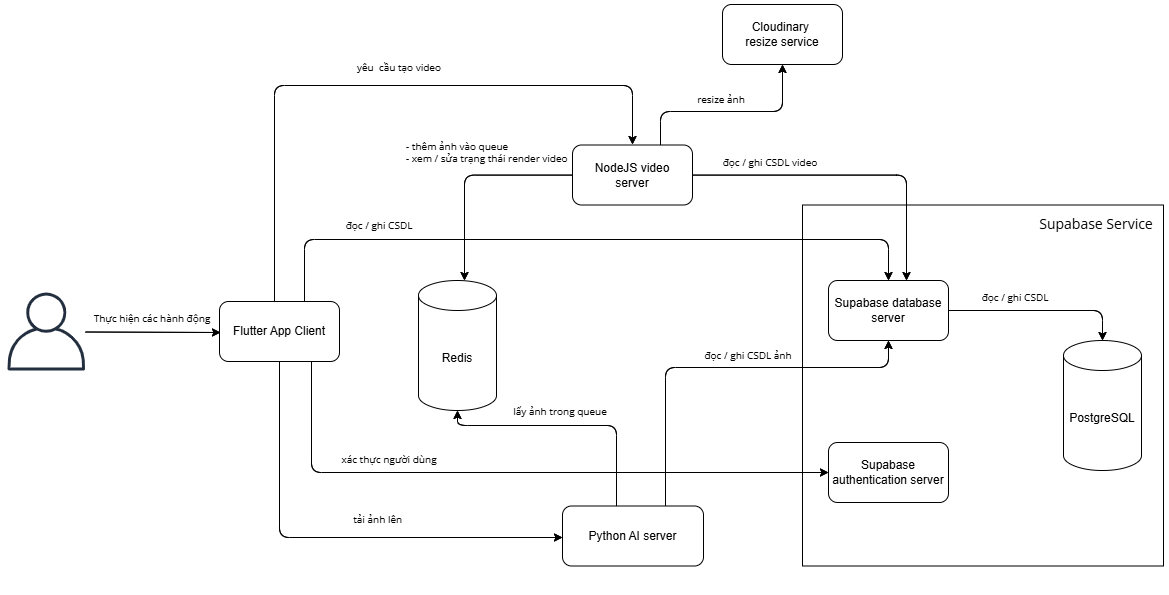
\includegraphics[width=1.1\textwidth]{figures/c4/4_1/architechture.png}
    \caption{Biểu đồ kiến trúc hệ thống.}
    \label{fig:architecture_diagram}
\end{figure}

\section{Các chức năng chính của hệ thống}

Chương này sẽ trình bày các chức năng chính của hệ thống, bao gồm các chức năng chính mà người dùng có thể sử dụng để tạo ra video slideshow từ bộ sưu tập ảnh của họ. Nội dung chương sẽ bao gồm mô tả chi tiết các chức năng kèm theo hình ảnh thực tế giao diện ứng dụng của hệ thống. Các chức năng chính của hệ thống bao gồm:

\subsection{Xác thực người dùng}

Hệ thống yêu cầu người dùng phải đăng nhập để sử dụng các chức năng của hệ thống như Hình \ref{fig:login-screen}. Người dùng tại đây có thể nhập tên tài khoản và mật khẩu đã đăng ký trước đó để truy cập vào hệ thống. 

Trường hợp người dùng chưa có tài khoản, hệ thống sẽ cung cấp chức năng đăng ký tài khoản mới có giao diện như Hình \ref{fig:signup-screen}.

\begin{figure}[H]
    \centering
    \begin{subfigure}{0.48\textwidth}
        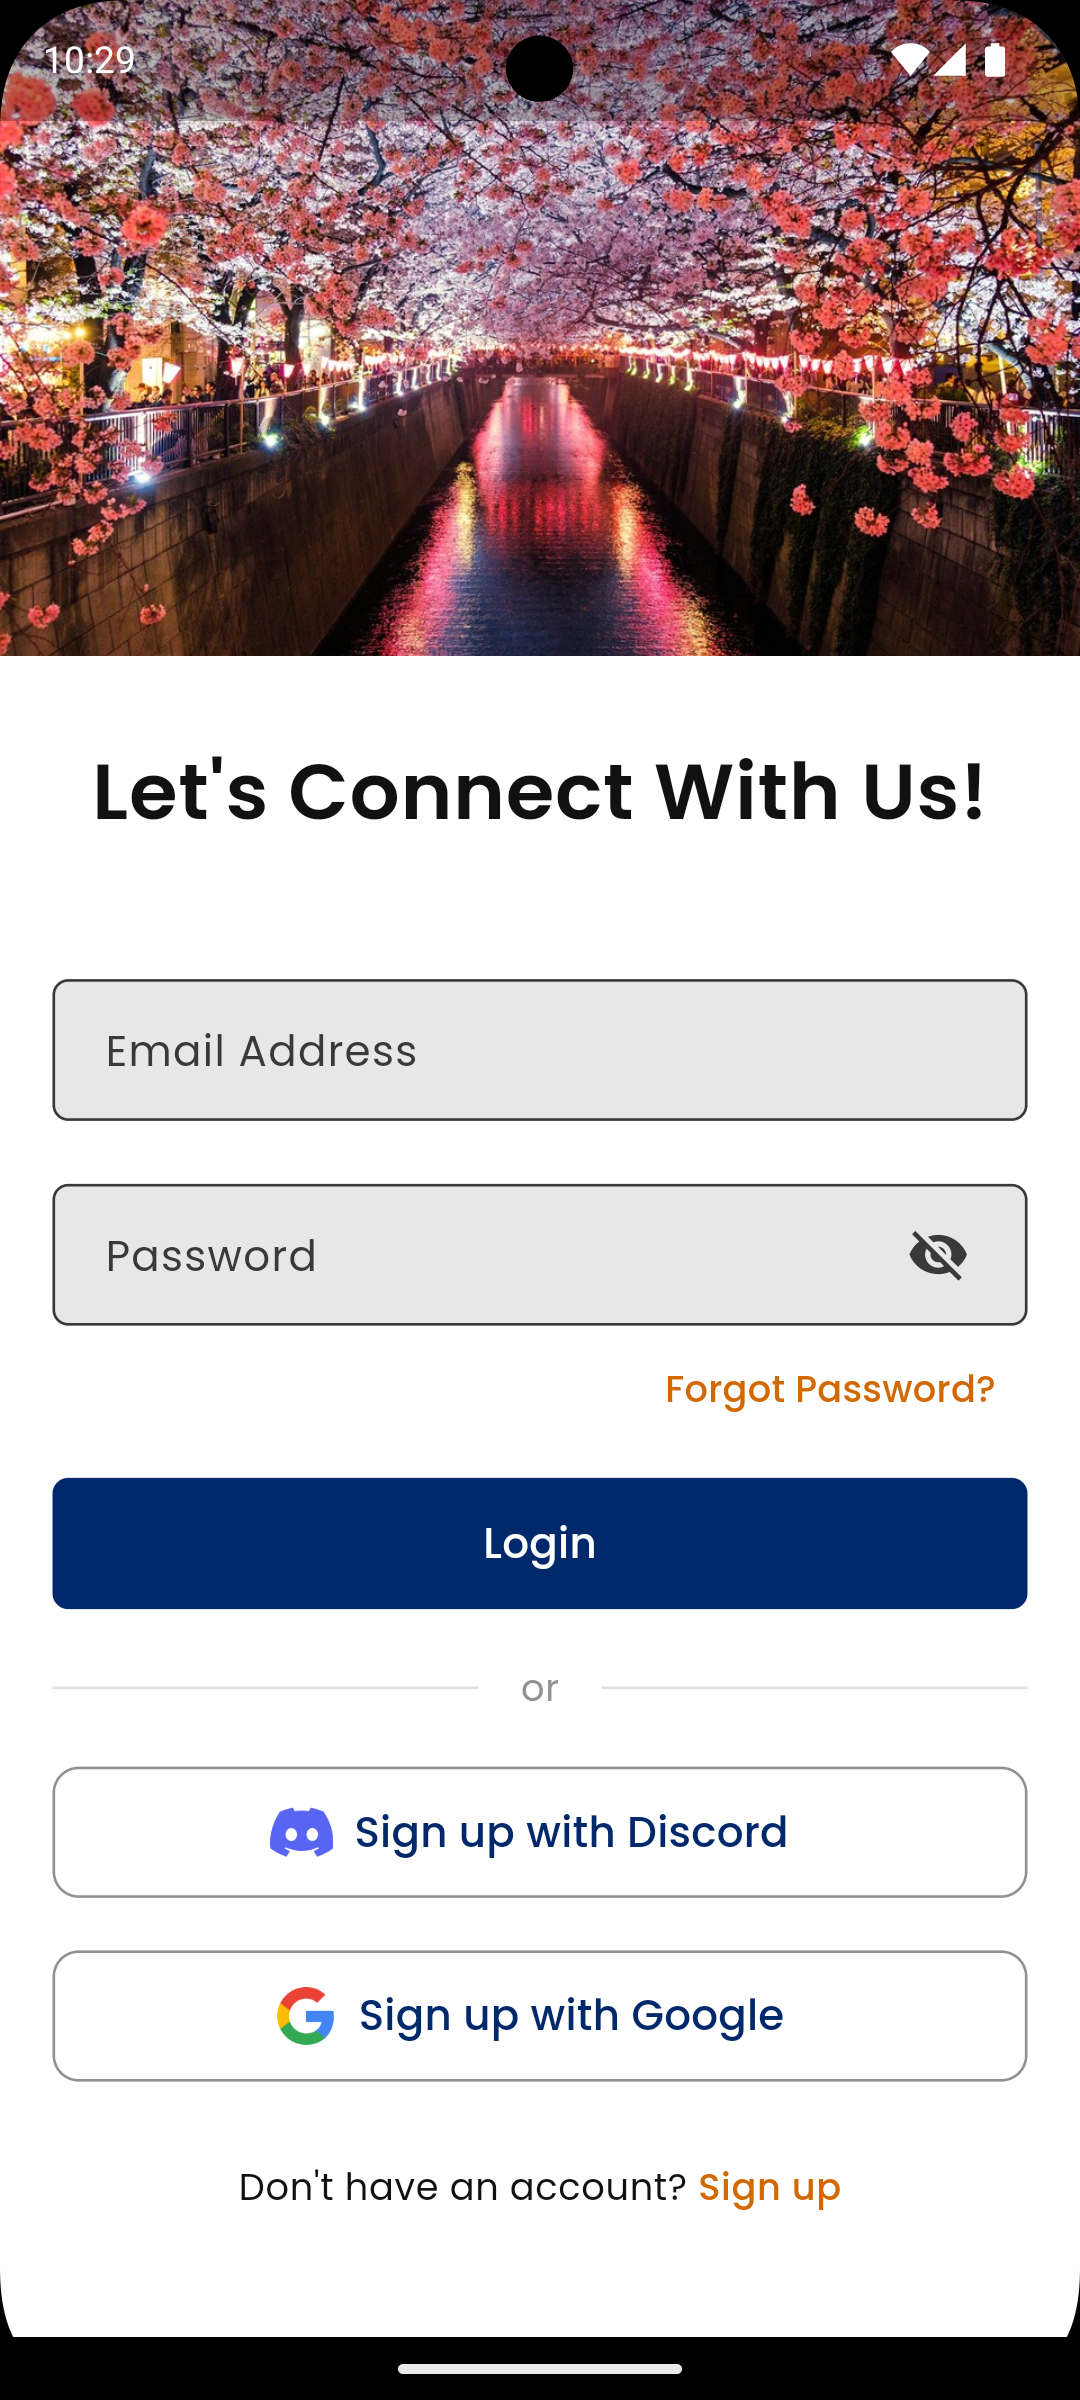
\includegraphics[width=1\linewidth]{figures/c4/4-2/login.png} 
        \caption{Giao diện đăng nhập}
        \label{fig:login-screen}
    \end{subfigure}
    \hfill
    \begin{subfigure}{0.48\textwidth}
        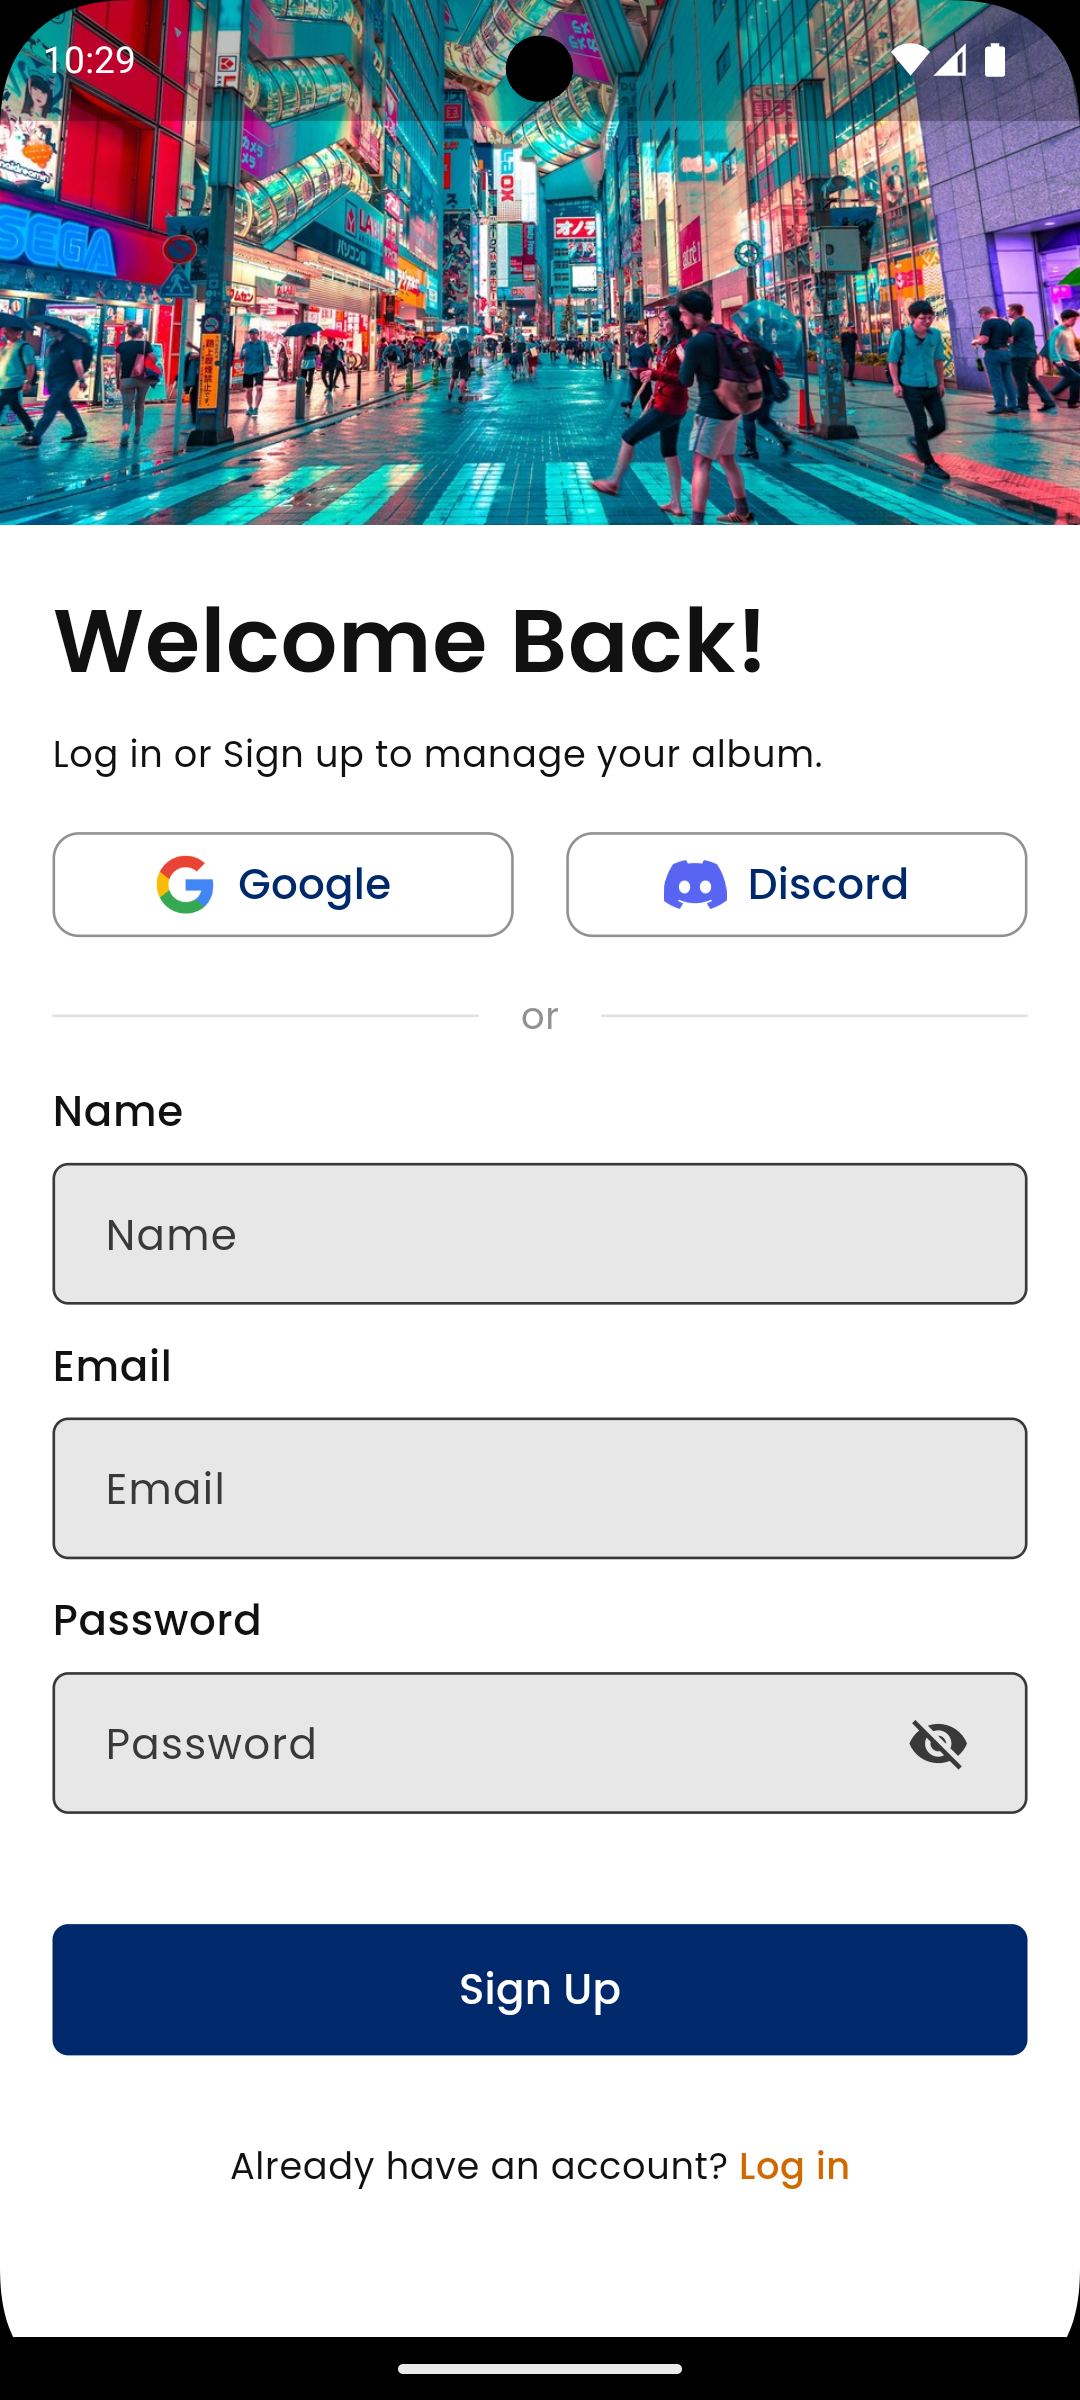
\includegraphics[width=1\linewidth]{figures/c4/4-2/sign_up.png} 
        \caption{Giao diện đăng ký}
        \label{fig:signup-screen}
    \end{subfigure}
    \caption{Giao diện xác thực người dùng.}
\end{figure}

Sau khi người dùng tạo tài khoản thành công, hệ thống sẽ điều hướng người dùng đến trang điền thông tin tài khoản như Hình \ref{fig:basic-information-screen}. Tại đây, người dùng sẽ phải điền ngày sinh, tên, ảnh đại diện, upload 1 số ảnh cá nhân và thực hiện khảo sát hệ thống trước khi tiến hành sử dụng chức năng chính của hệ thống.

\begin{figure}[H]
    \centering
    \begin{subfigure}{0.32\textwidth}
        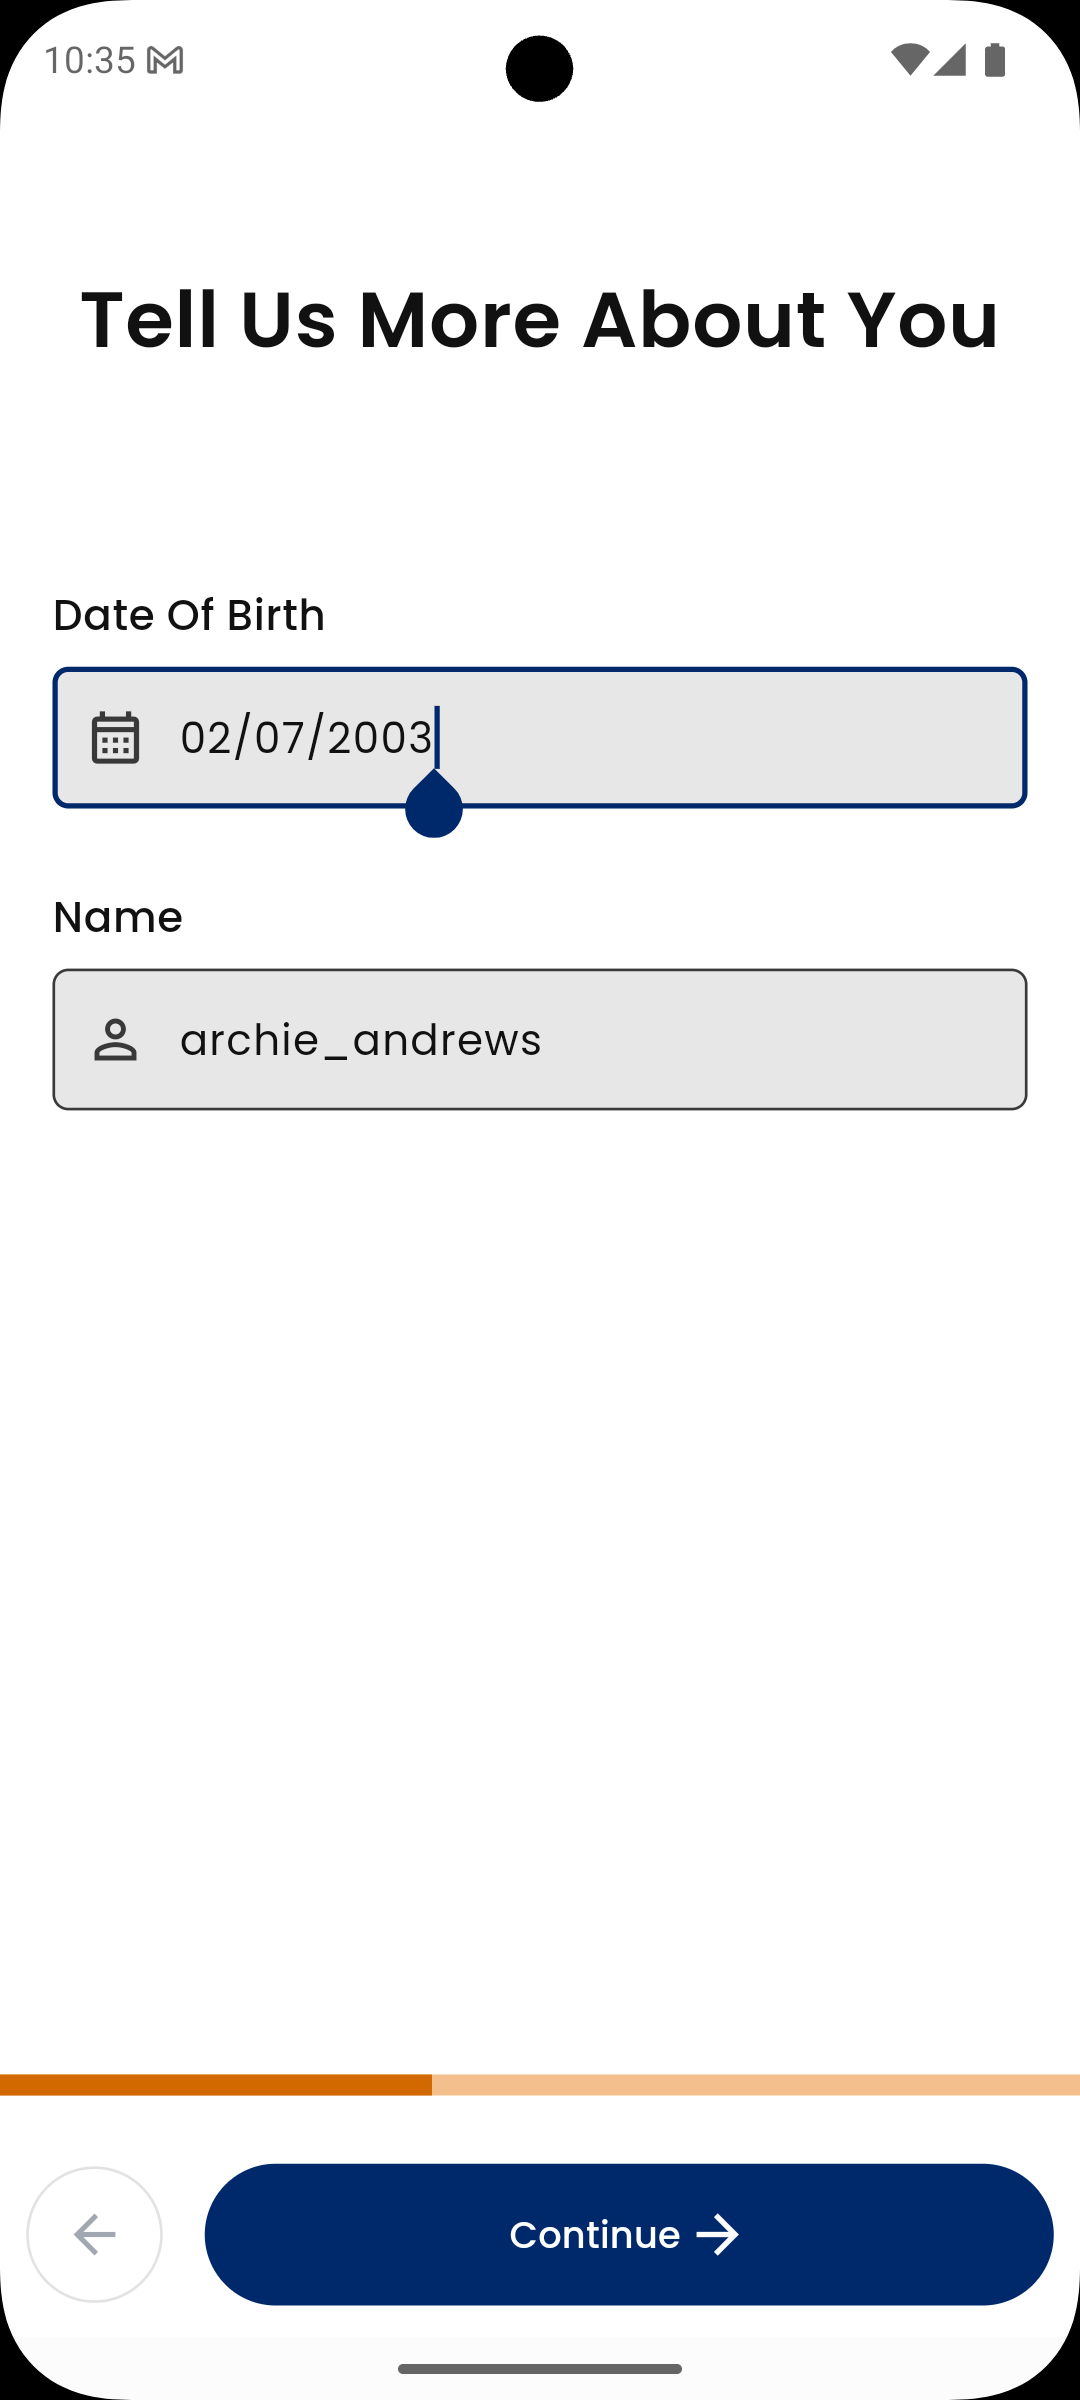
\includegraphics[width=1\linewidth]{figures/c4/4-2/basic_info_2.png} 
        \caption{Form thông tin cá nhân}
        \label{fig:basic-info}
    \end{subfigure}
    \hfill
    \begin{subfigure}{0.32\textwidth}
        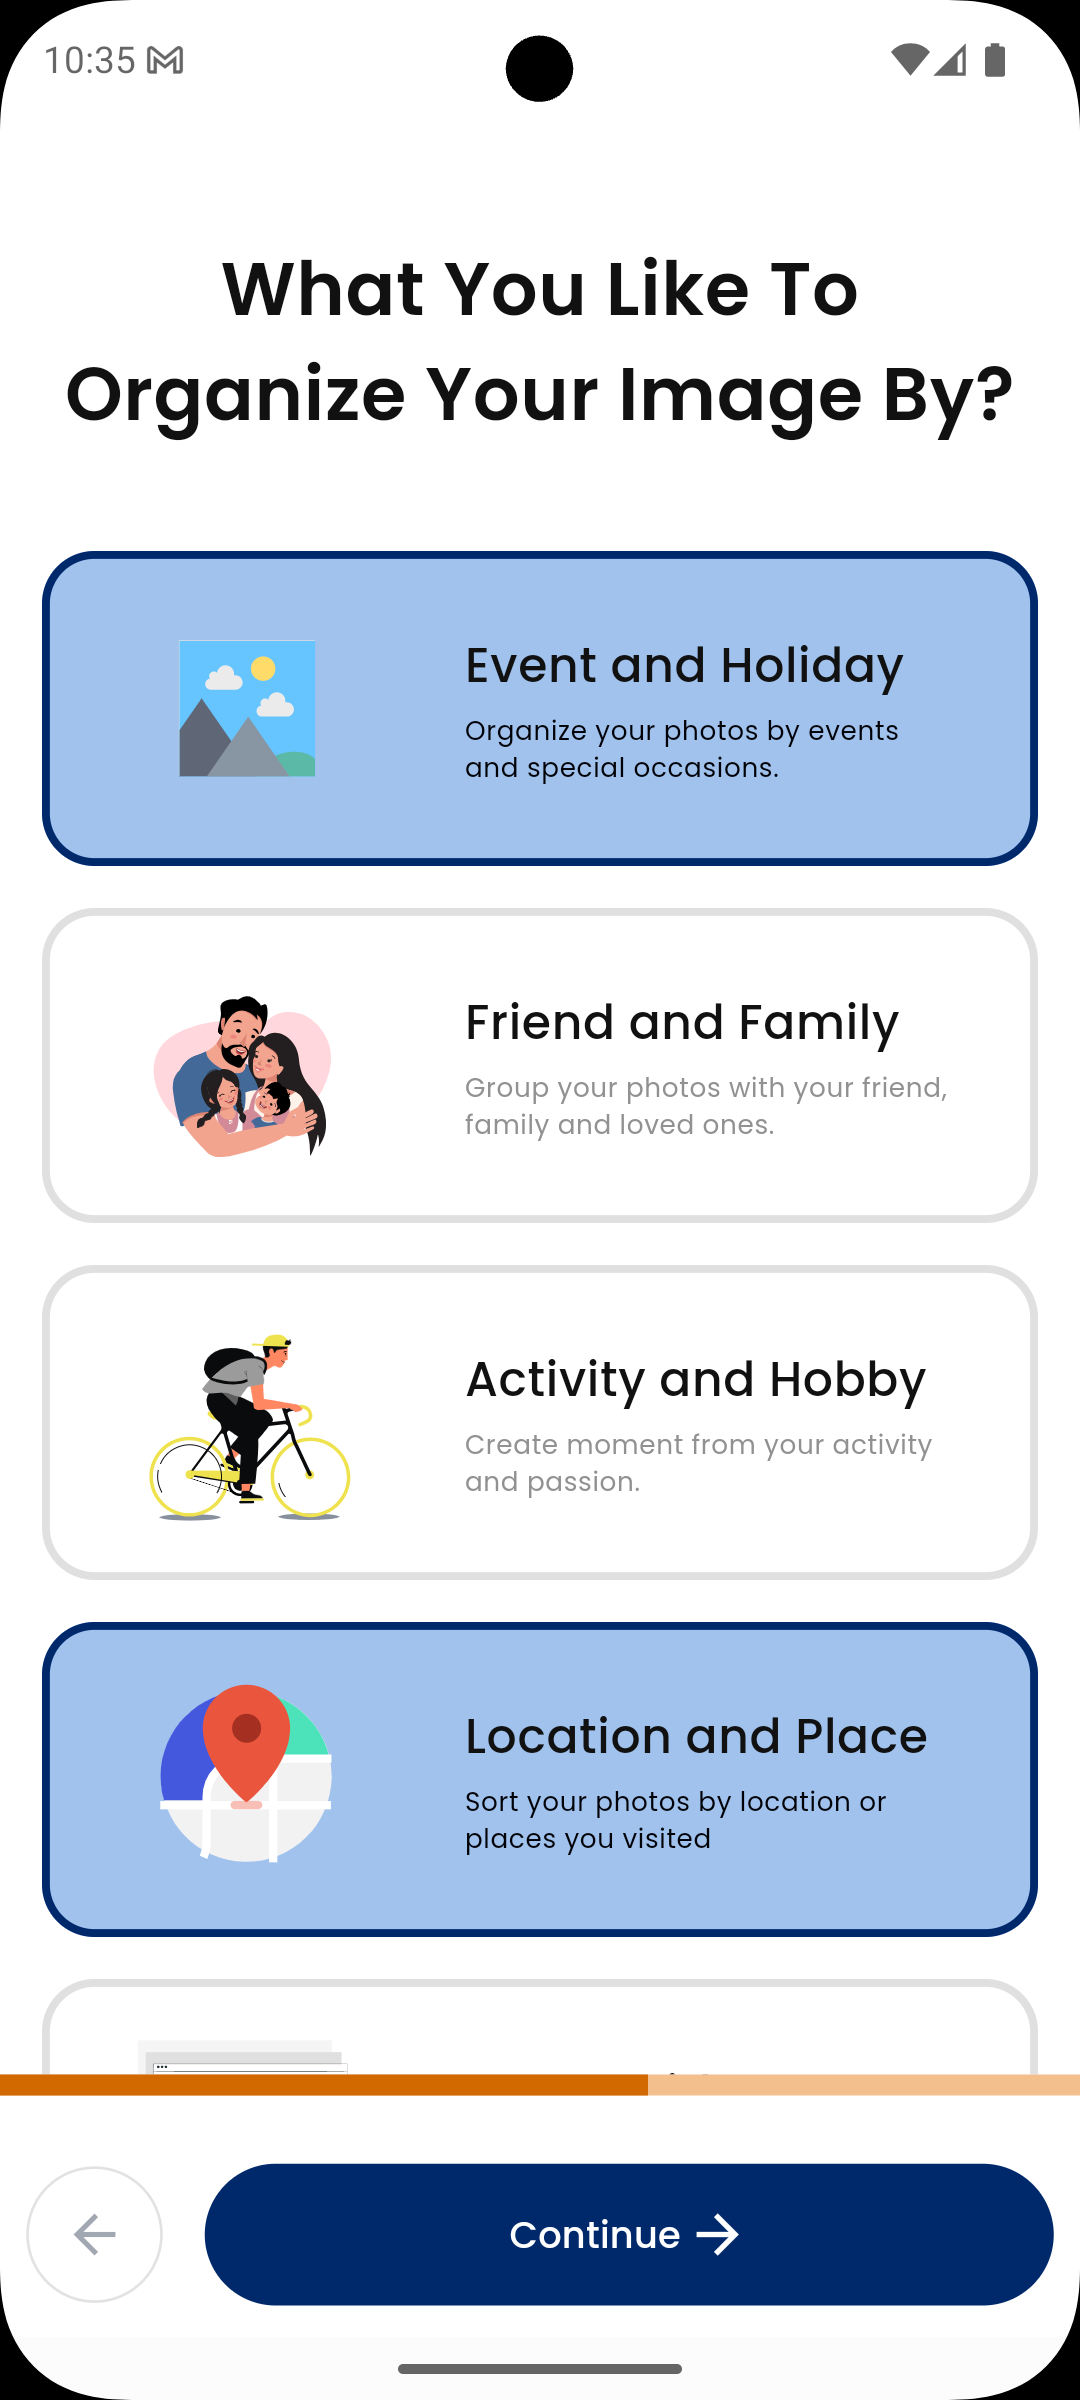
\includegraphics[width=1\linewidth]{figures/c4/4-2/basic_info_3.png} 
        \caption{Form khảo sát}
        \label{fig:upload-form}
    \end{subfigure}
    \hfill
    \begin{subfigure}{0.32\textwidth}
        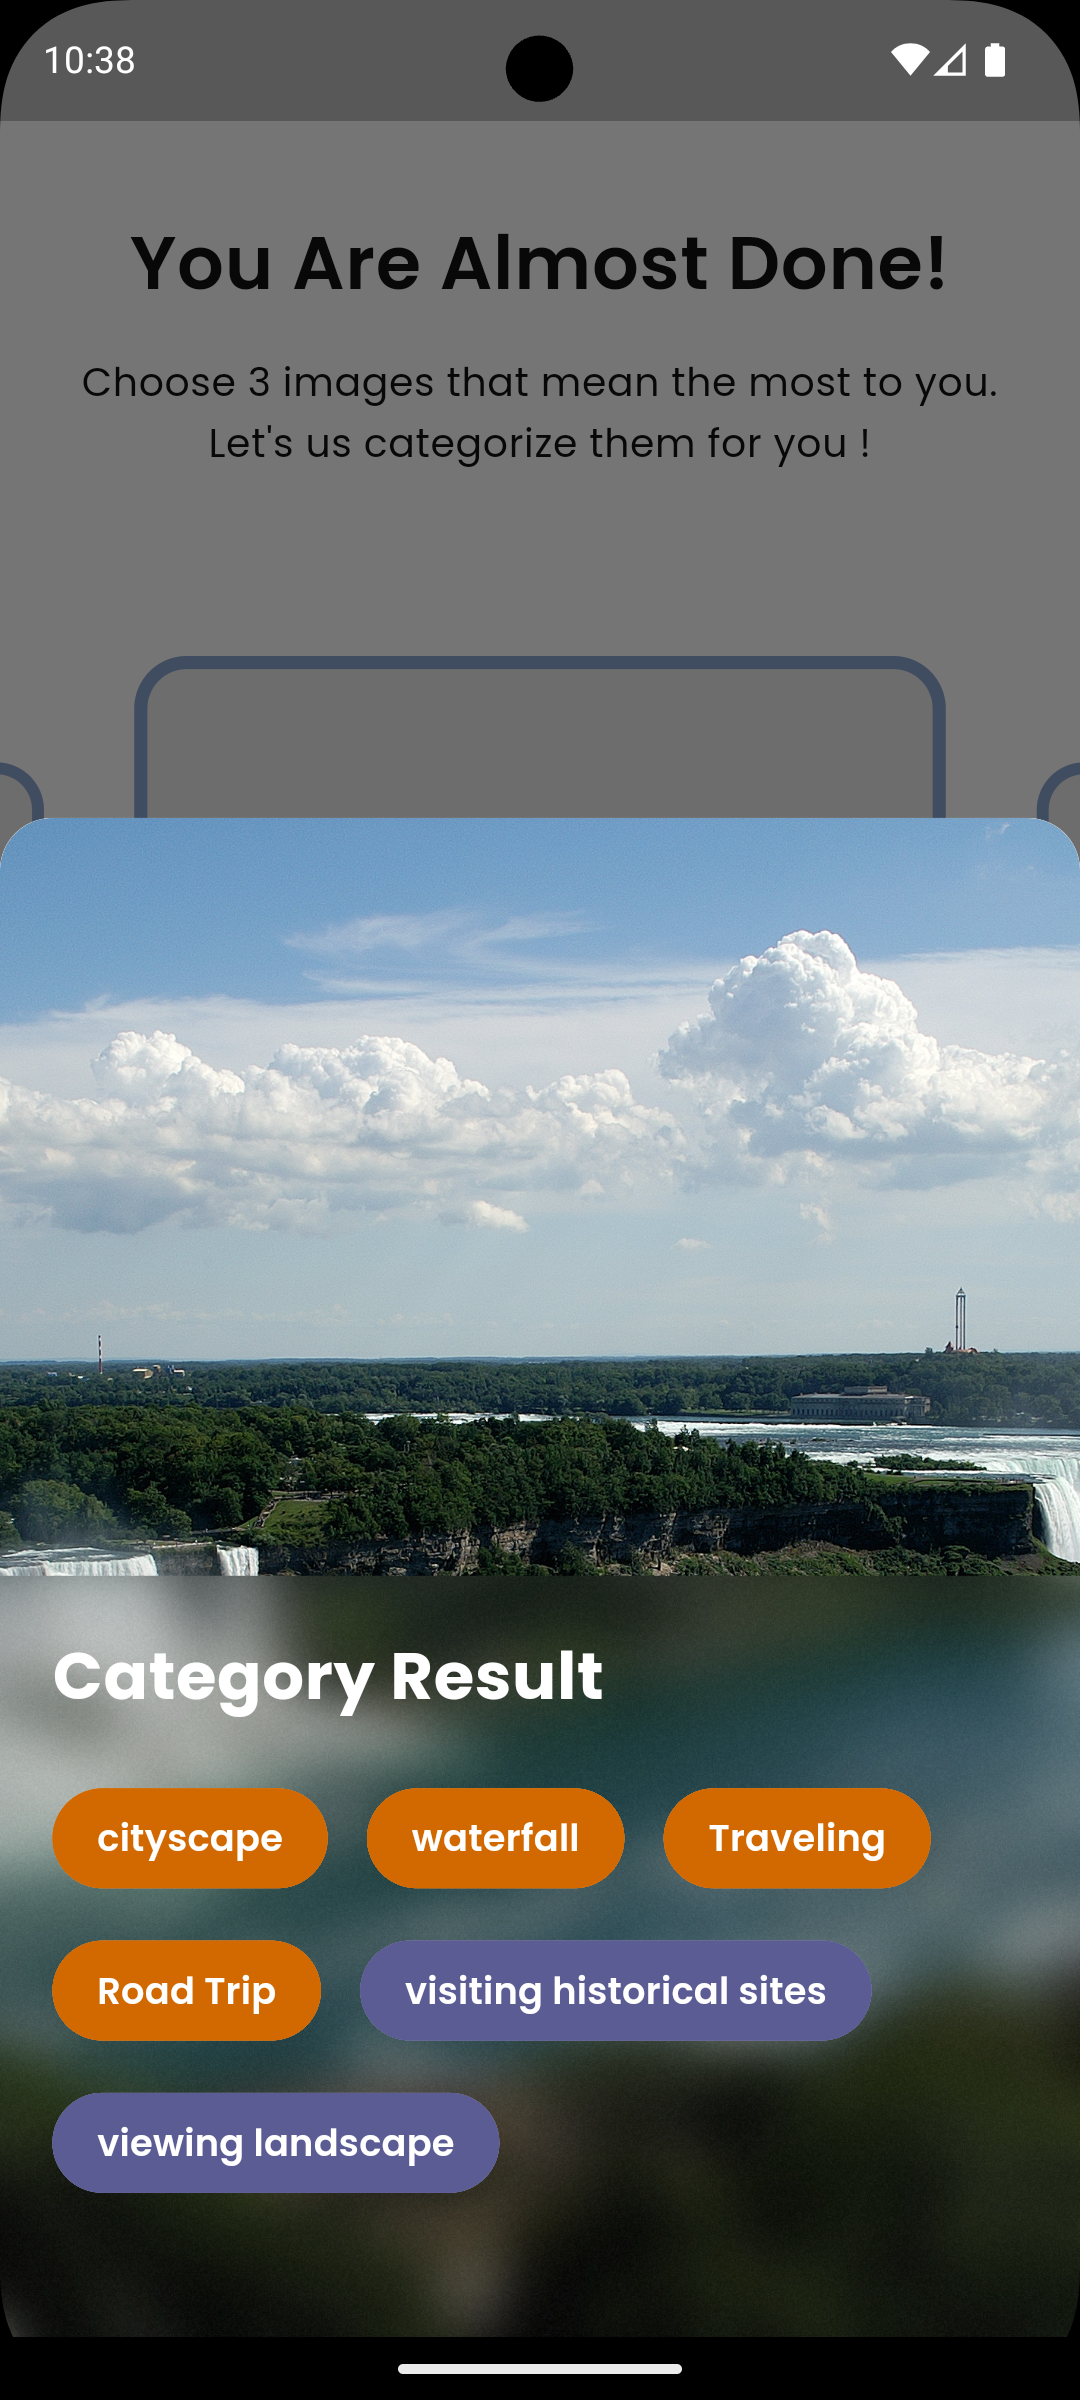
\includegraphics[width=1\linewidth]{figures/c4/4-2/basic_info_4.png} 
        \caption{Form kết quả upload ảnh}
        \label{fig:survey-form}
    \end{subfigure}
    \caption{Giao diện điền thông tin người dùng.}
    \label{fig:basic-information-screen}
\end{figure}

Sau khi đăng ký tài khoản, người dùng có thể kiểm tra thông tin cá nhân tại màn hình thông tin cá nhân như Hình \ref{fig:profile-screen}. 

\begin{figure}[H]
    \centering  
    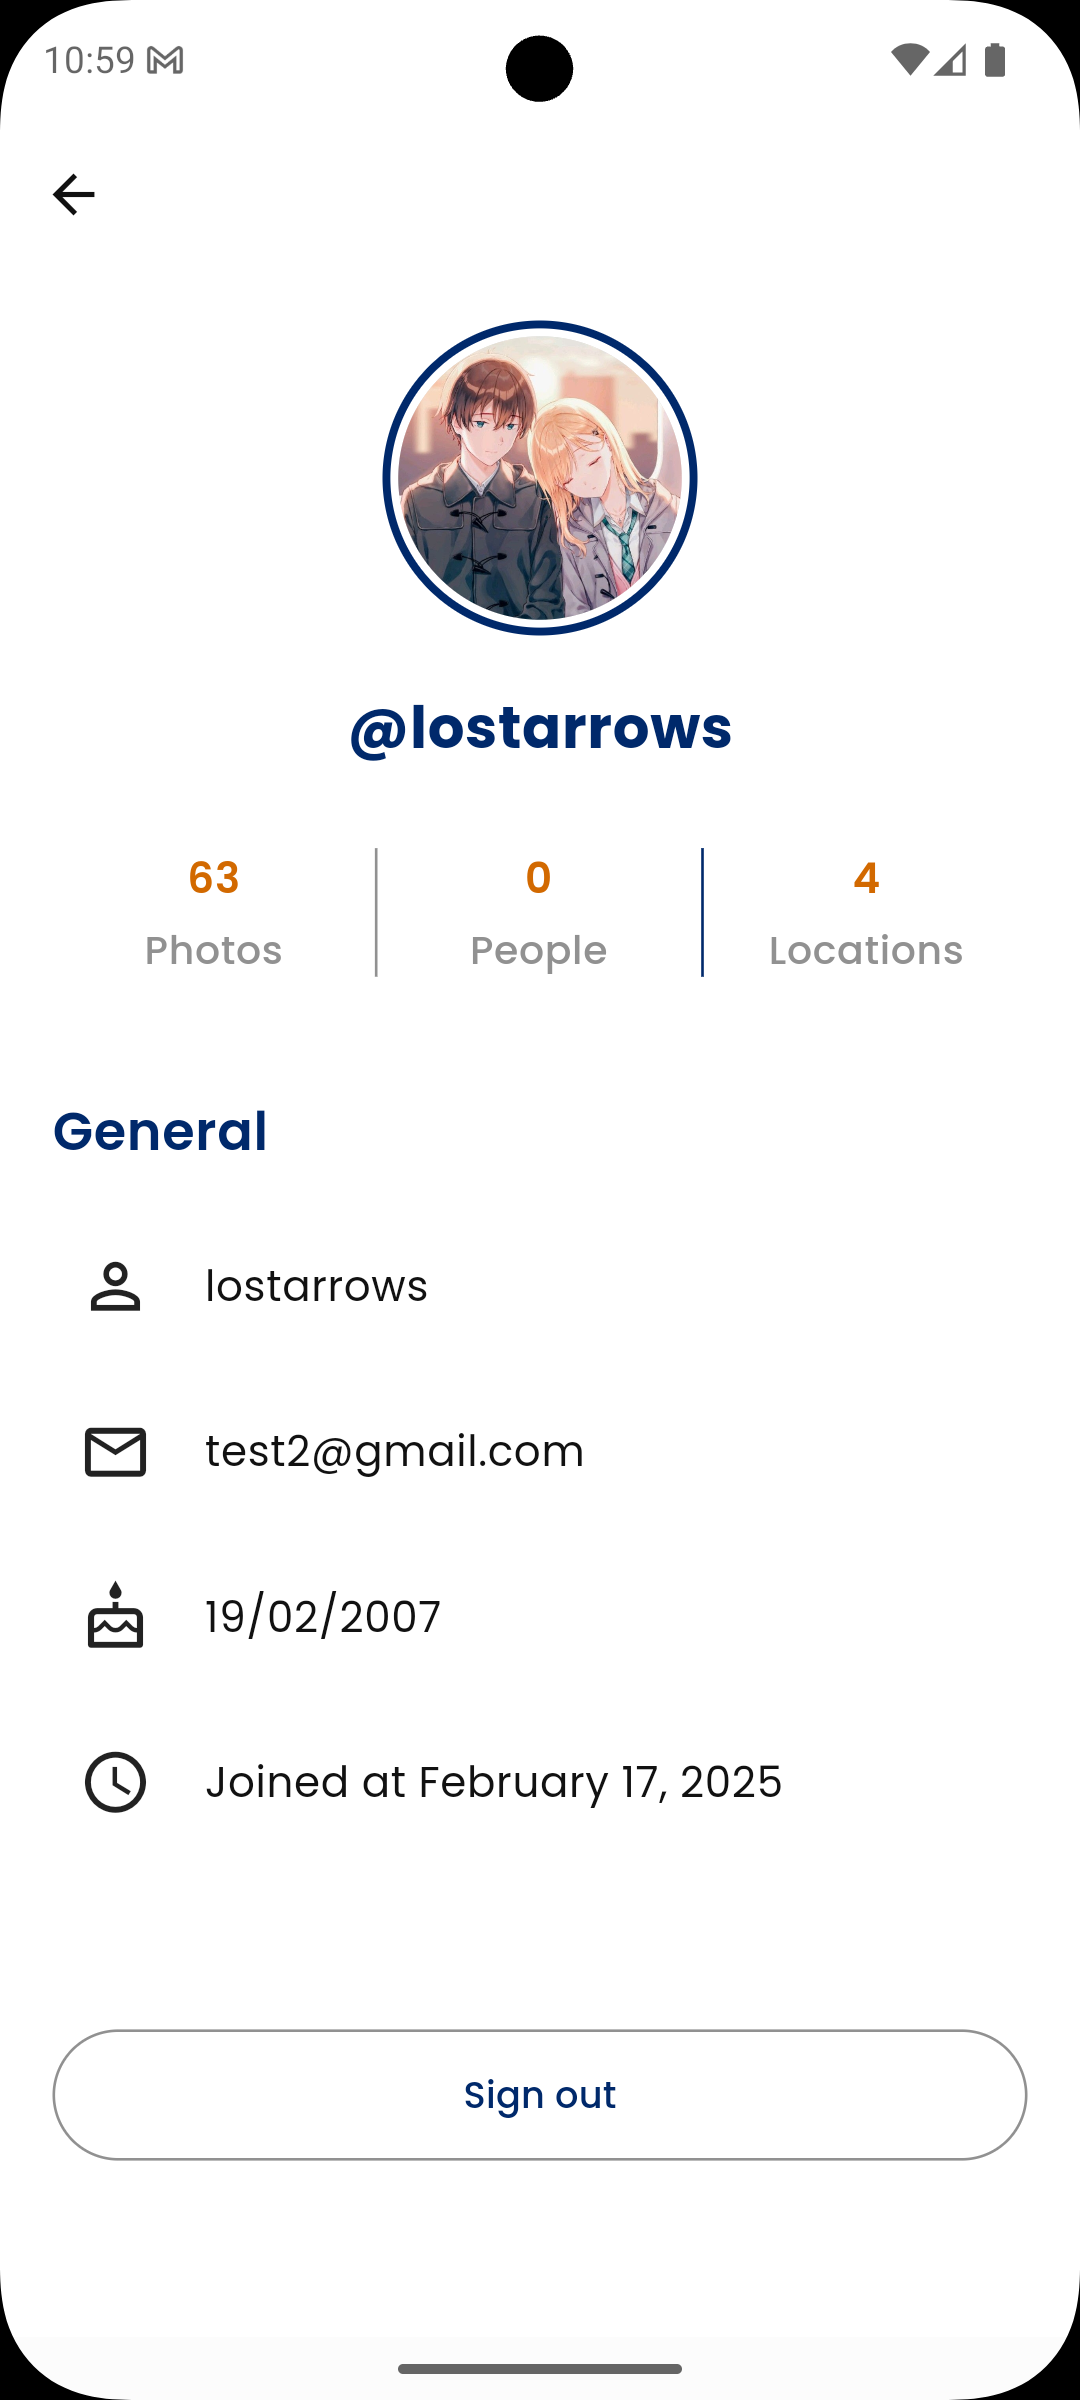
\includegraphics[width=0.5\textwidth]{figures/c4/4-2/profile.png}
    \caption{Giao diện thông tin cá nhân.}
    \label{fig:profile-screen}
\end{figure}

\subsection{Quản lý ảnh}

Sau khi đăng nhập thành công, hệ thống sẽ điều hướng người dùng đến trang chủ thư viện ảnh, nơi người dùng có thể xem các ảnh đã tải lên theo ngày / tháng / năm như hình \ref{fig:gallery}.

\begin{figure}[H]
    \centering
    \begin{subfigure}{0.48\textwidth}
        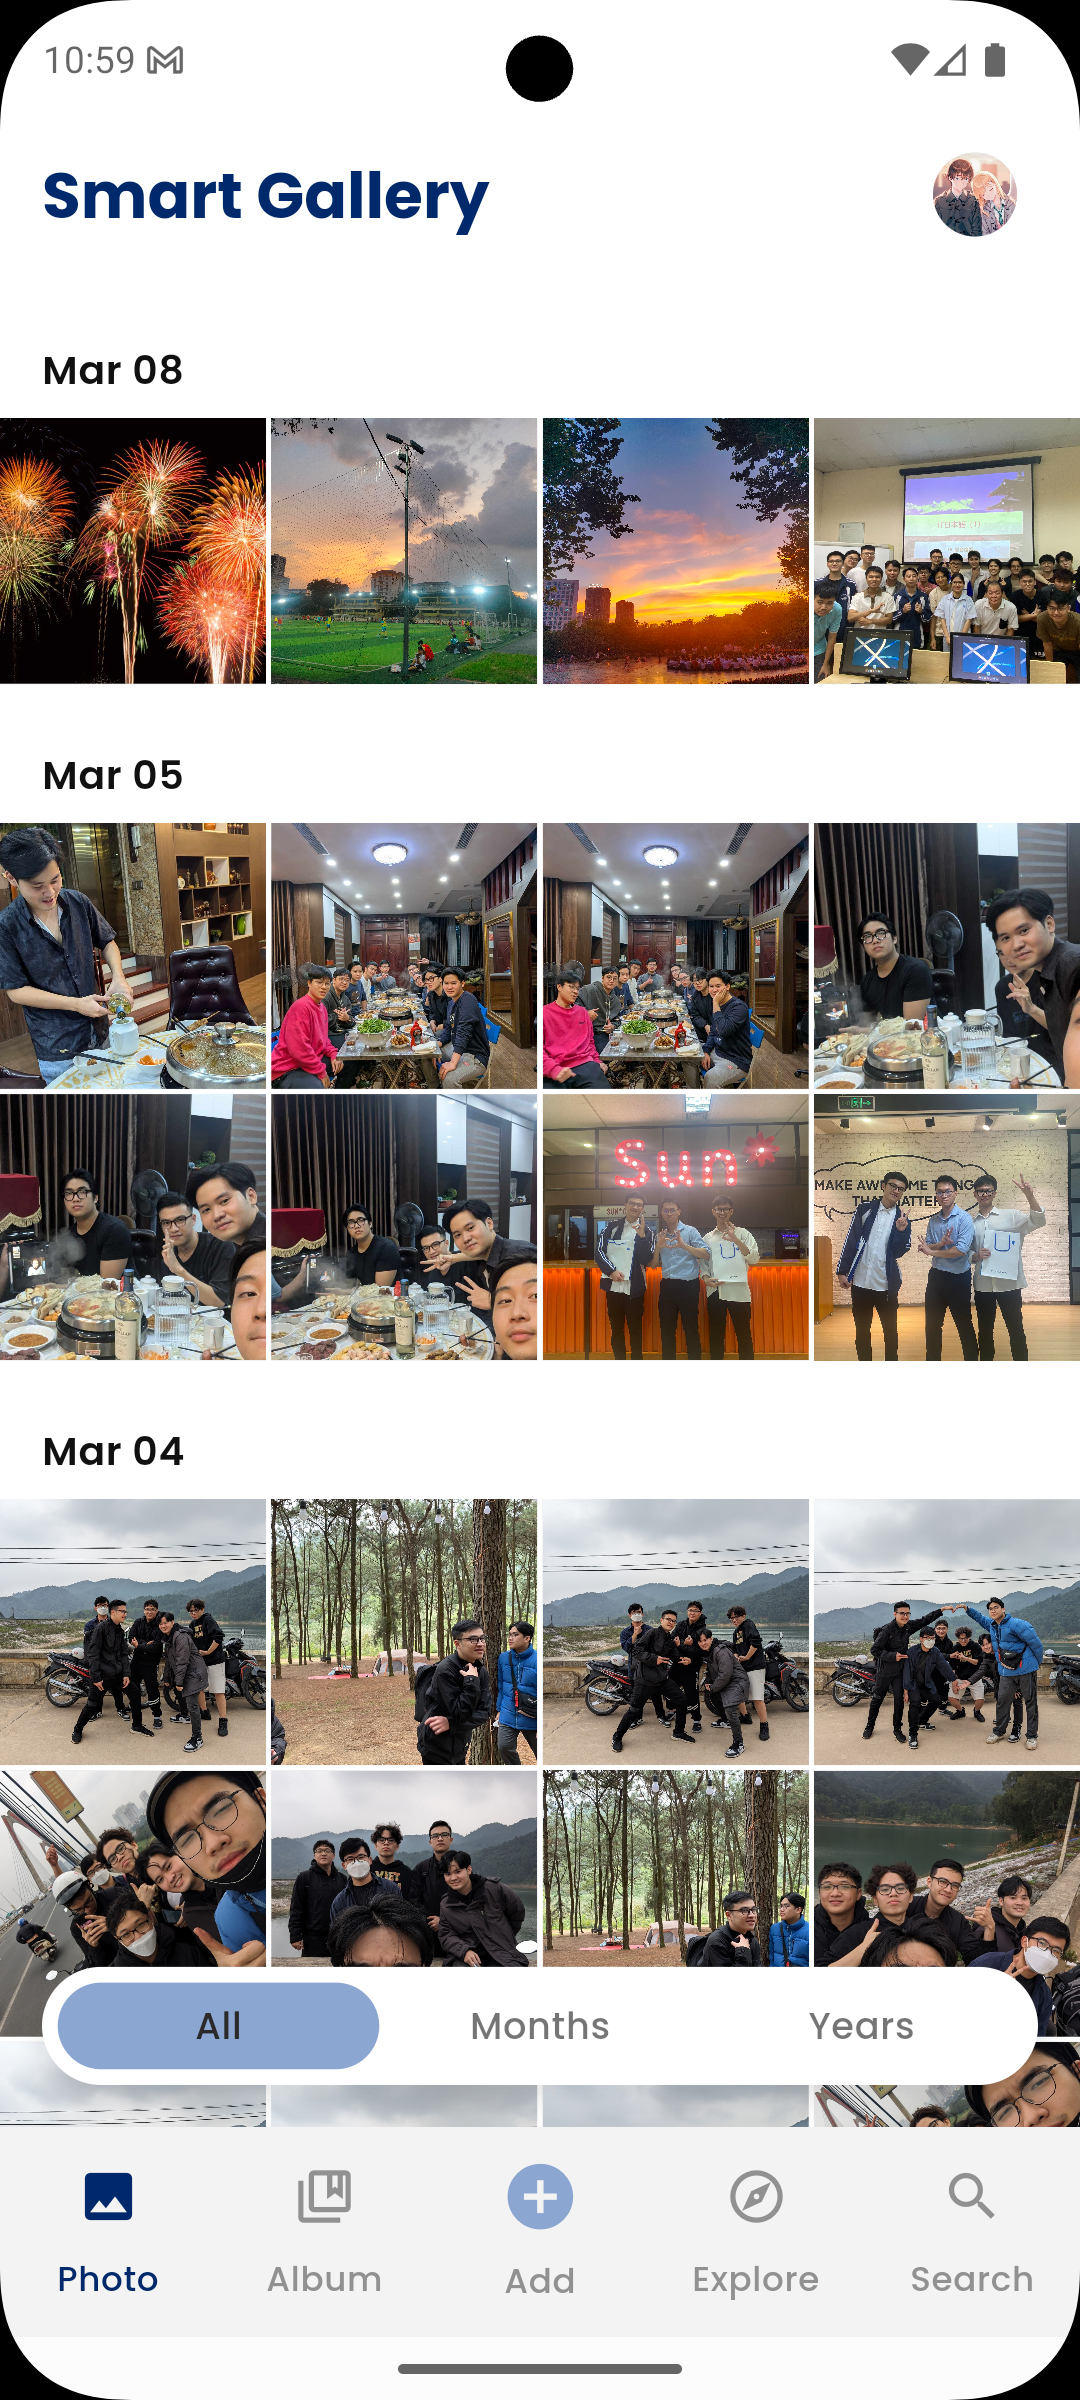
\includegraphics[width=1\linewidth]{figures/c4/4-2/gallery_1.png} 
        \caption{Xem ảnh theo ngày}
    \end{subfigure}
    \hfill
    \begin{subfigure}{0.48\textwidth}
        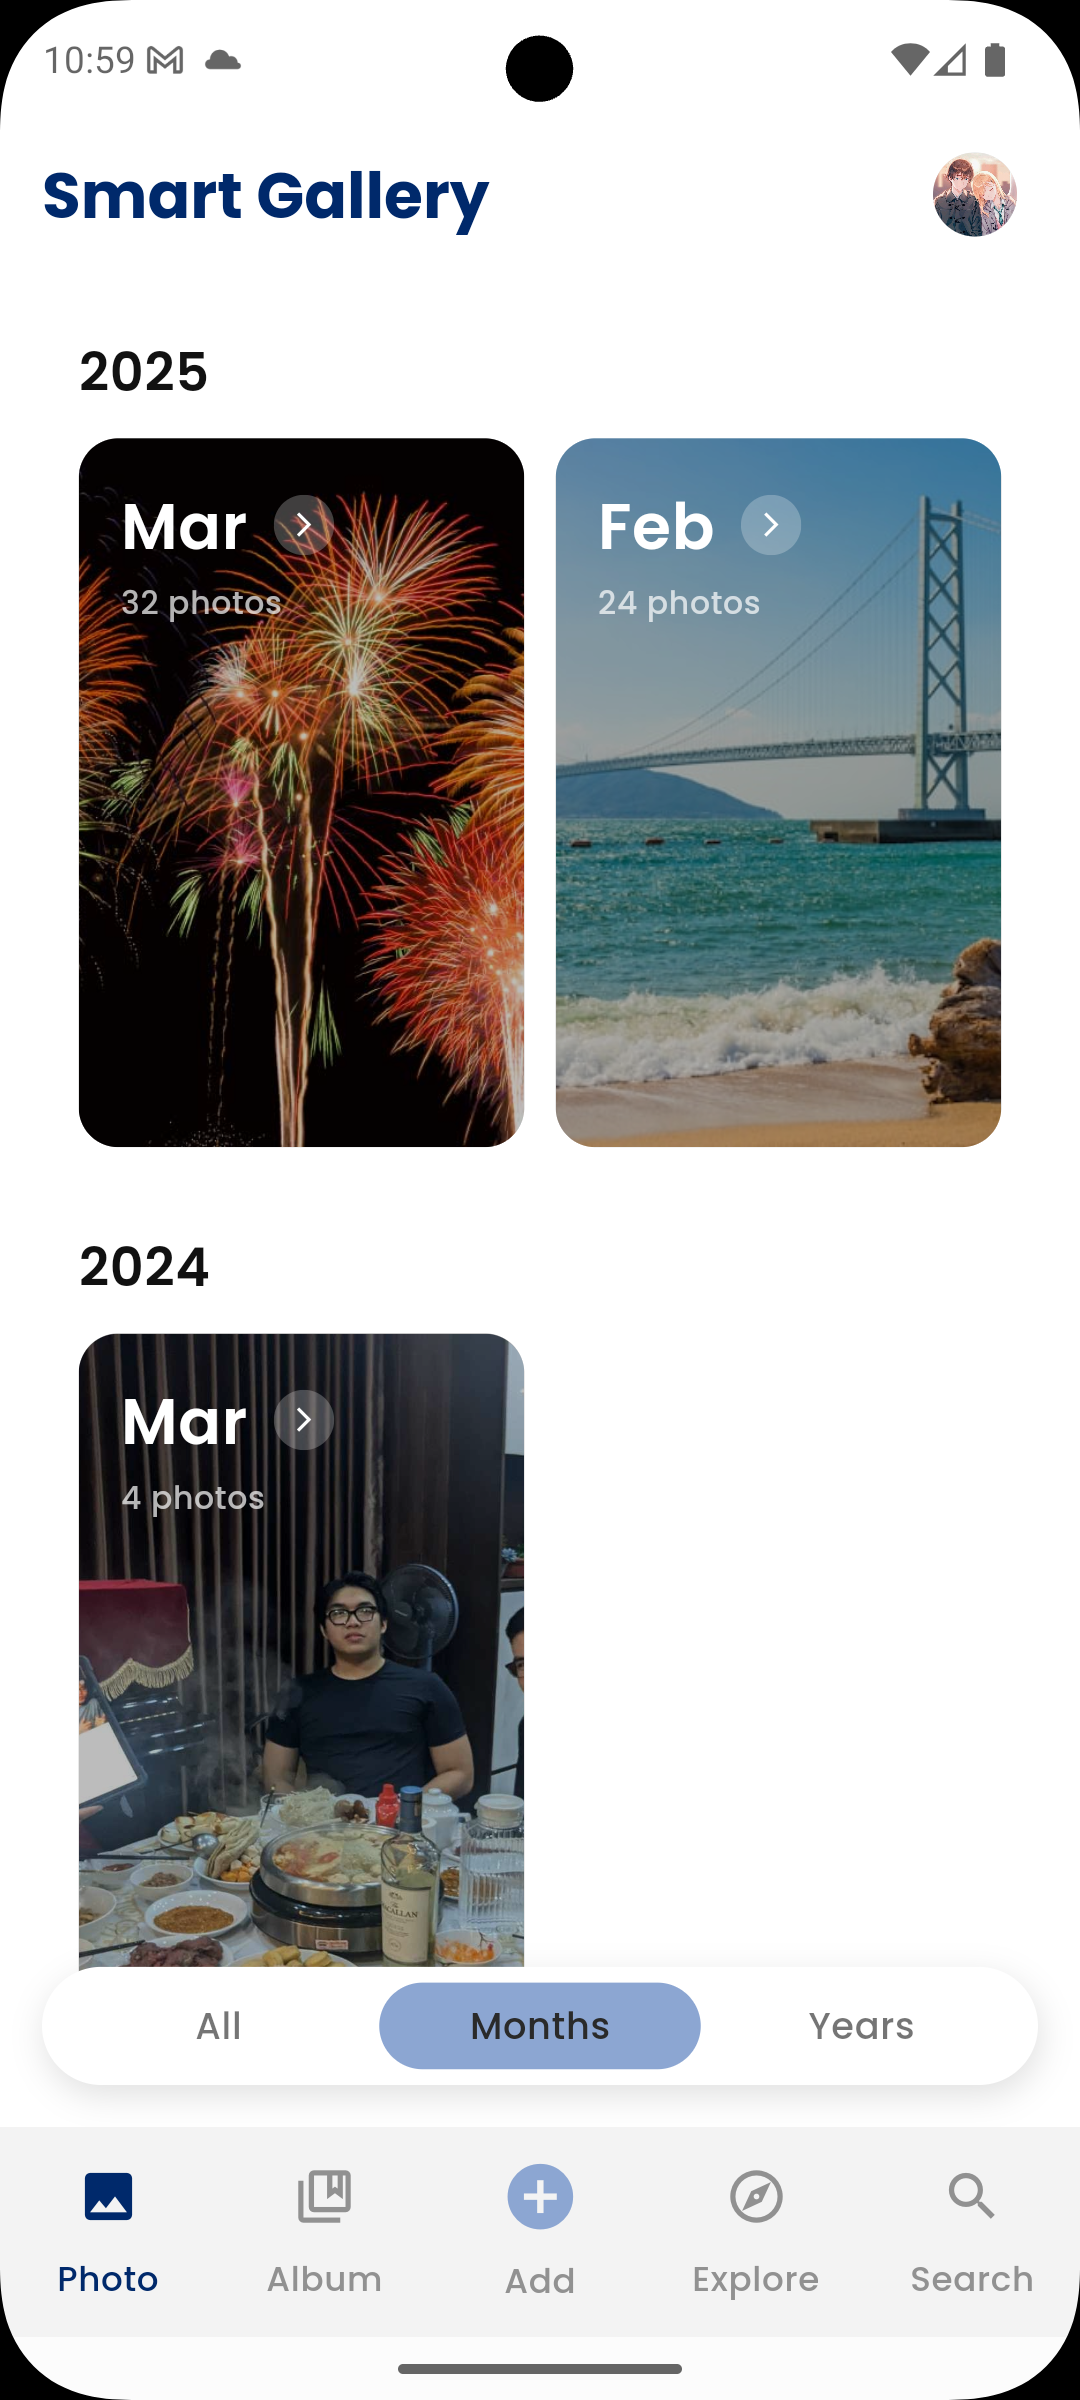
\includegraphics[width=1\linewidth]{figures/c4/4-2/gallery_2.png} 
        \caption{Xem ảnh theo tháng}
    \end{subfigure}
    \caption{Giao diện thư viện ảnh.}
    \label{fig:gallery}
\end{figure}

Người dùng có thể bấm vào từng ảnh để xem thông tin như hình \ref{fig:photo-info}. Tại đây, người dùng có thể thực hiện các chức năng như xóa ảnh, yêu thích ảnh, đổi tên ảnh và xem thông tin chi tiết của ảnh như thời gian chụp, vị trí chụp, các tag liên quan đến ảnh và các khuôn mặt được nhận diện trong ảnh.

\begin{figure}[H]
    \centering
    \begin{subfigure}{0.48\textwidth}
        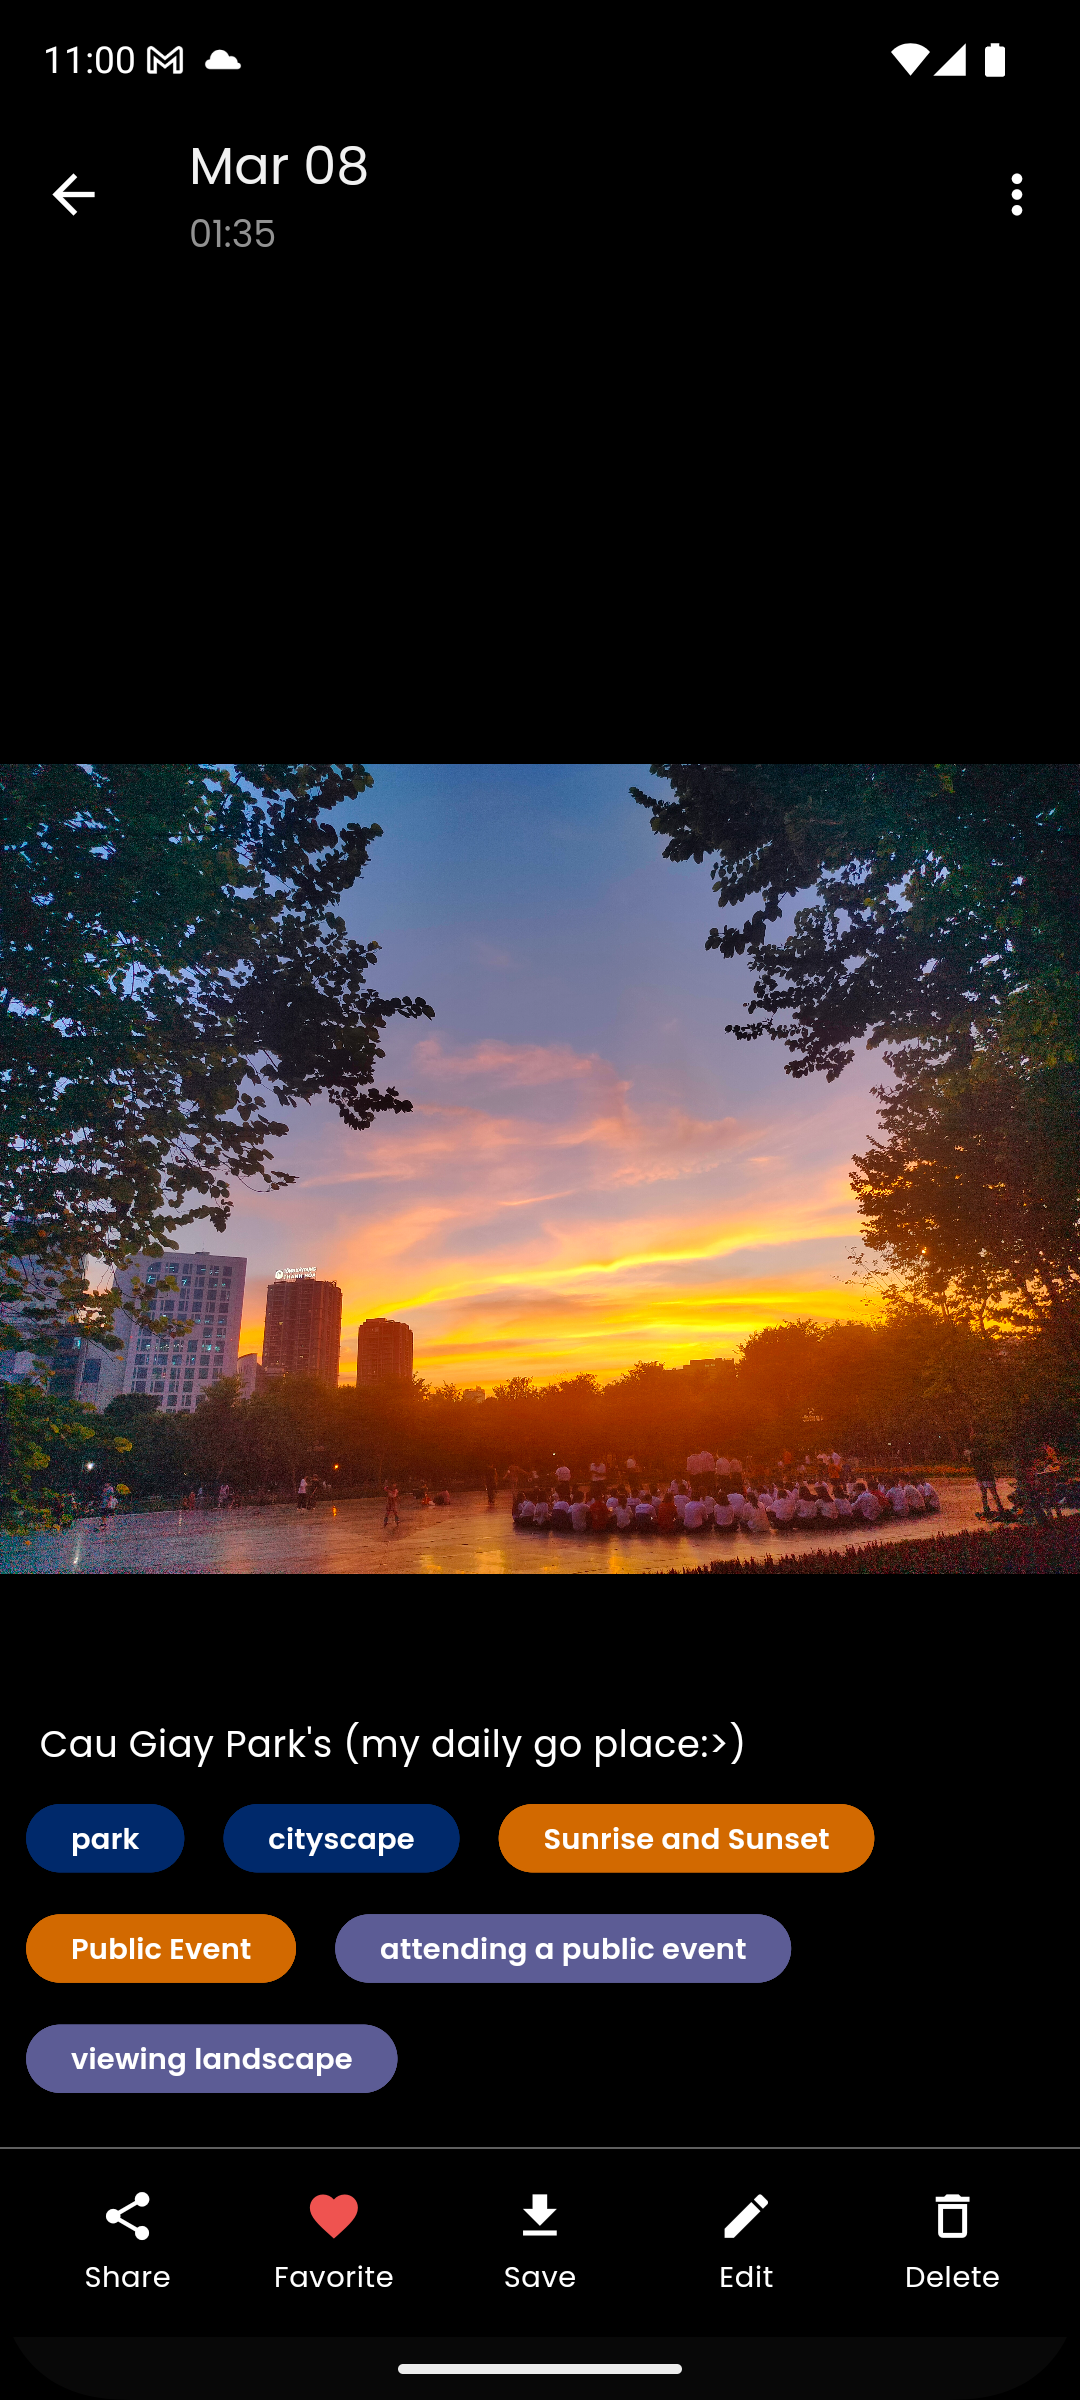
\includegraphics[width=1\linewidth]{figures/c4/4-2/image.png} 
        \caption{Xem ảnh}
    \end{subfigure}
    \hfill
    \begin{subfigure}{0.48\textwidth}
        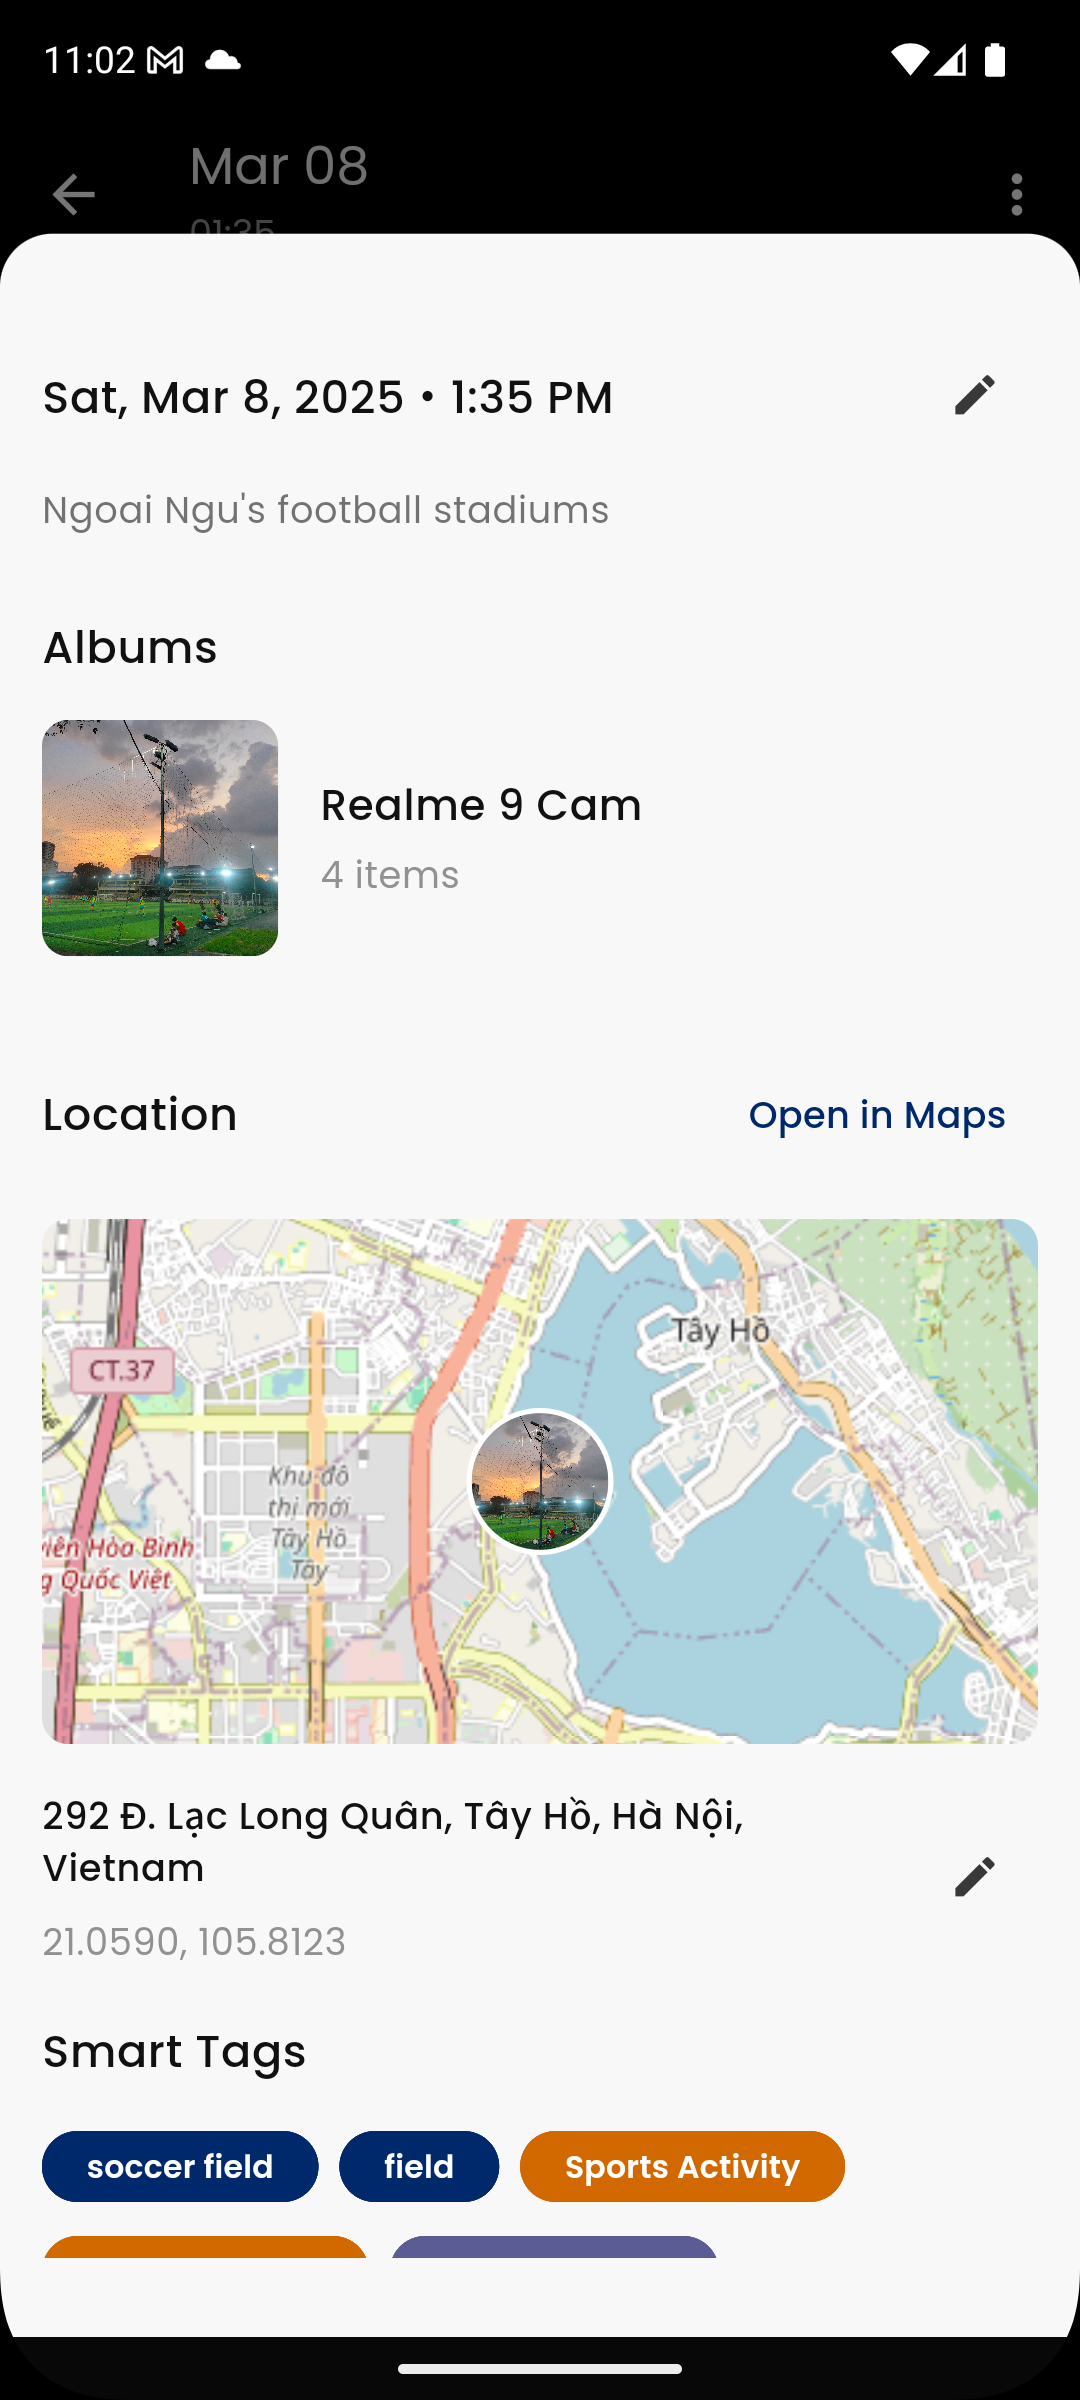
\includegraphics[width=1\linewidth]{figures/c4/4-2/image_info.png} 
        \caption{Xem thông tin }
    \end{subfigure}
    \caption{Giao diện thư viện ảnh.}
    \label{fig:photo-info}
\end{figure}

\subsection{Quản lý album ảnh}

Người dùng có thể quản lý, nhóm ảnh theo các album, xem danh sách các ảnh trong album đó và tạo album như Hình \ref{fig:album}. Tại đây người dùng có thể xem danh sách các album đã tạo, tải album về máy hay xóa album.

\begin{figure}[H]
    \centering
    \begin{subfigure}{0.32\textwidth}
        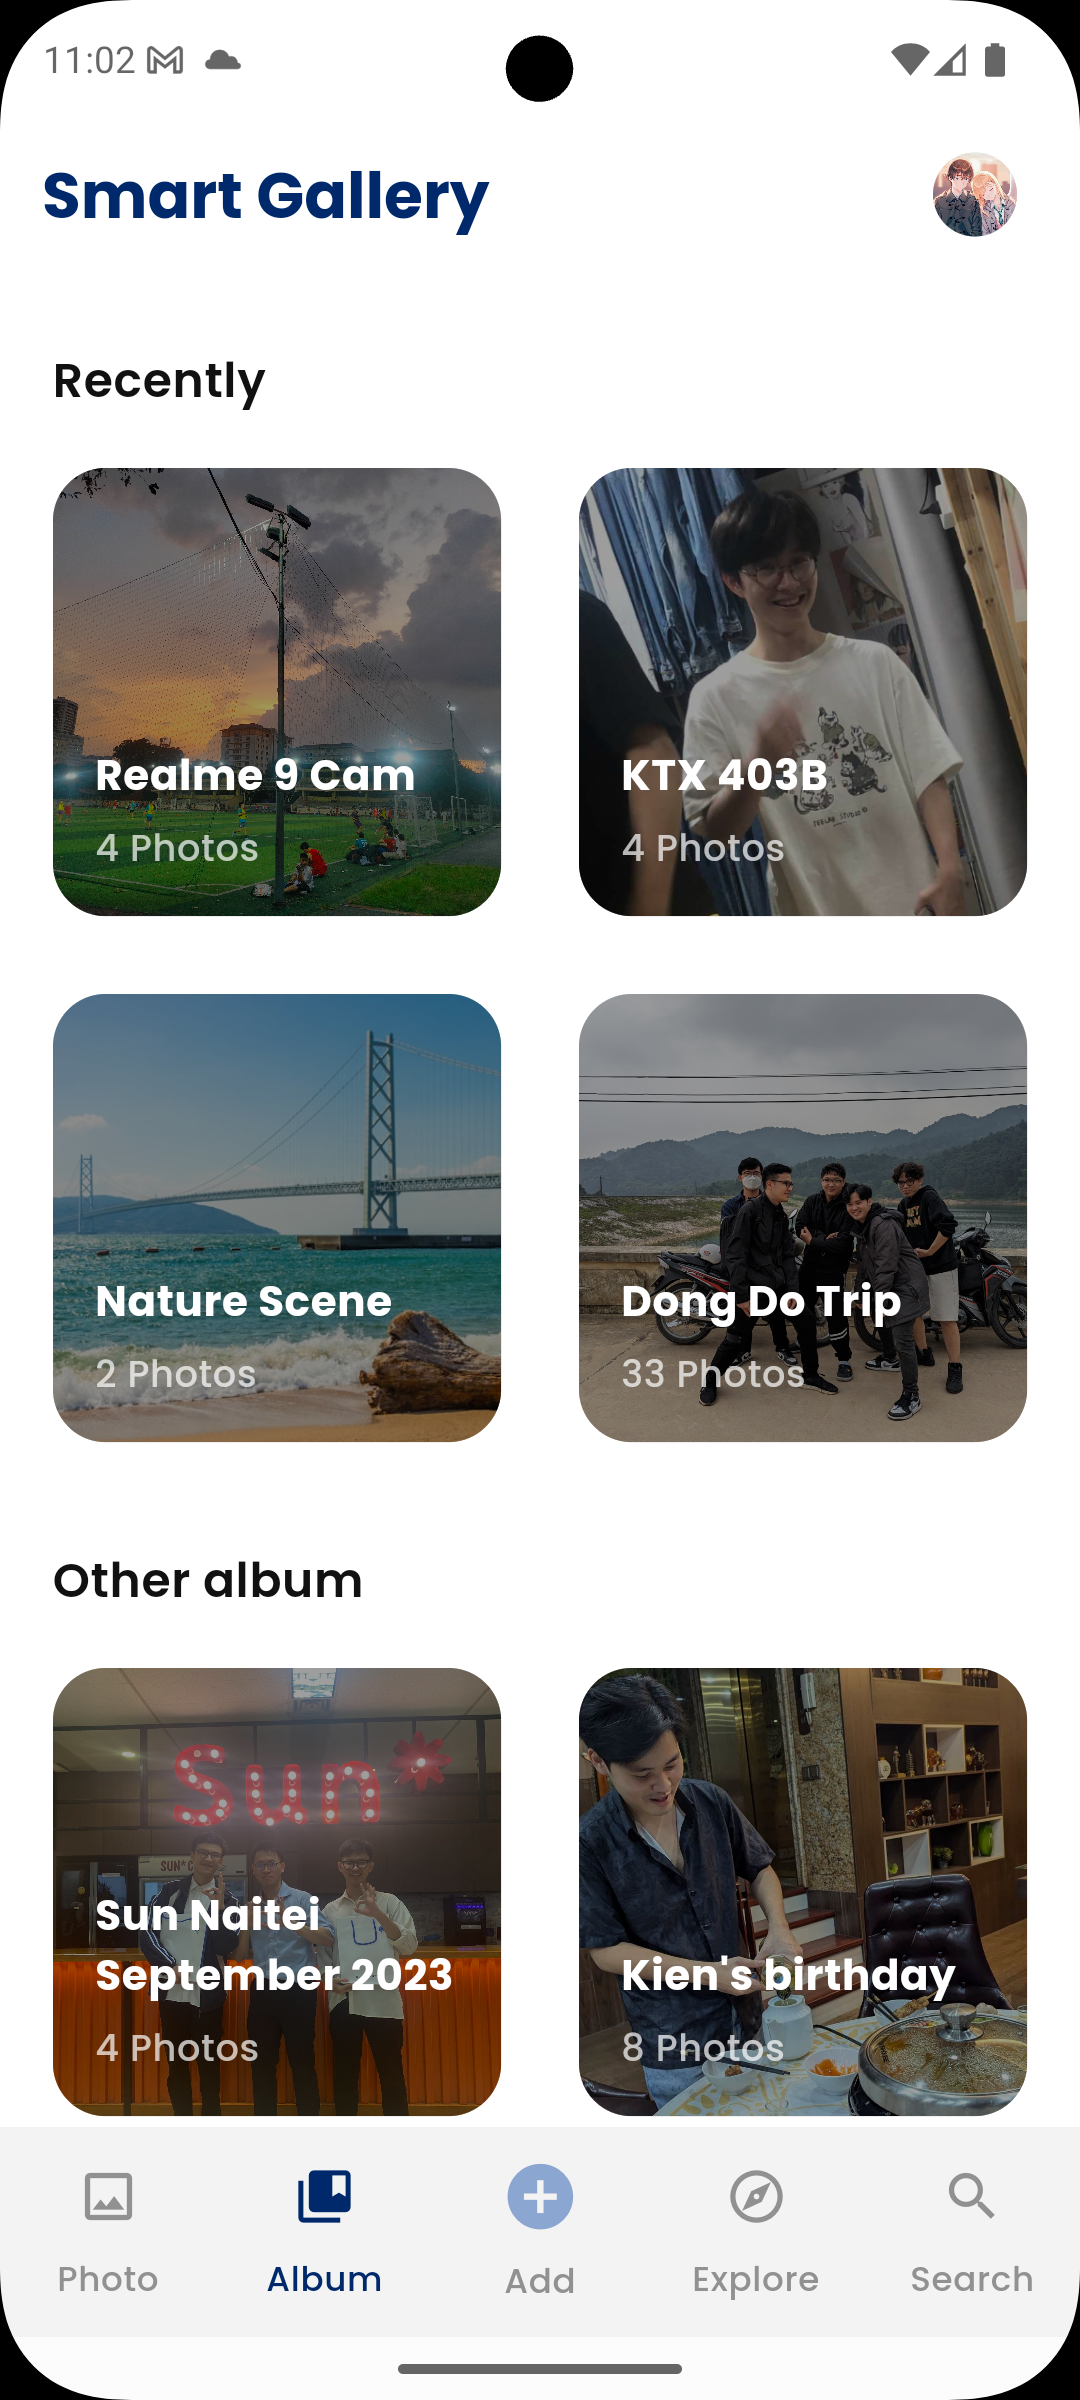
\includegraphics[width=1\linewidth]{figures/c4/4-2/album_1.png} 
        \caption{Danh sách album ảnh}
    \end{subfigure}
    \hfill
    \begin{subfigure}{0.32\textwidth}
        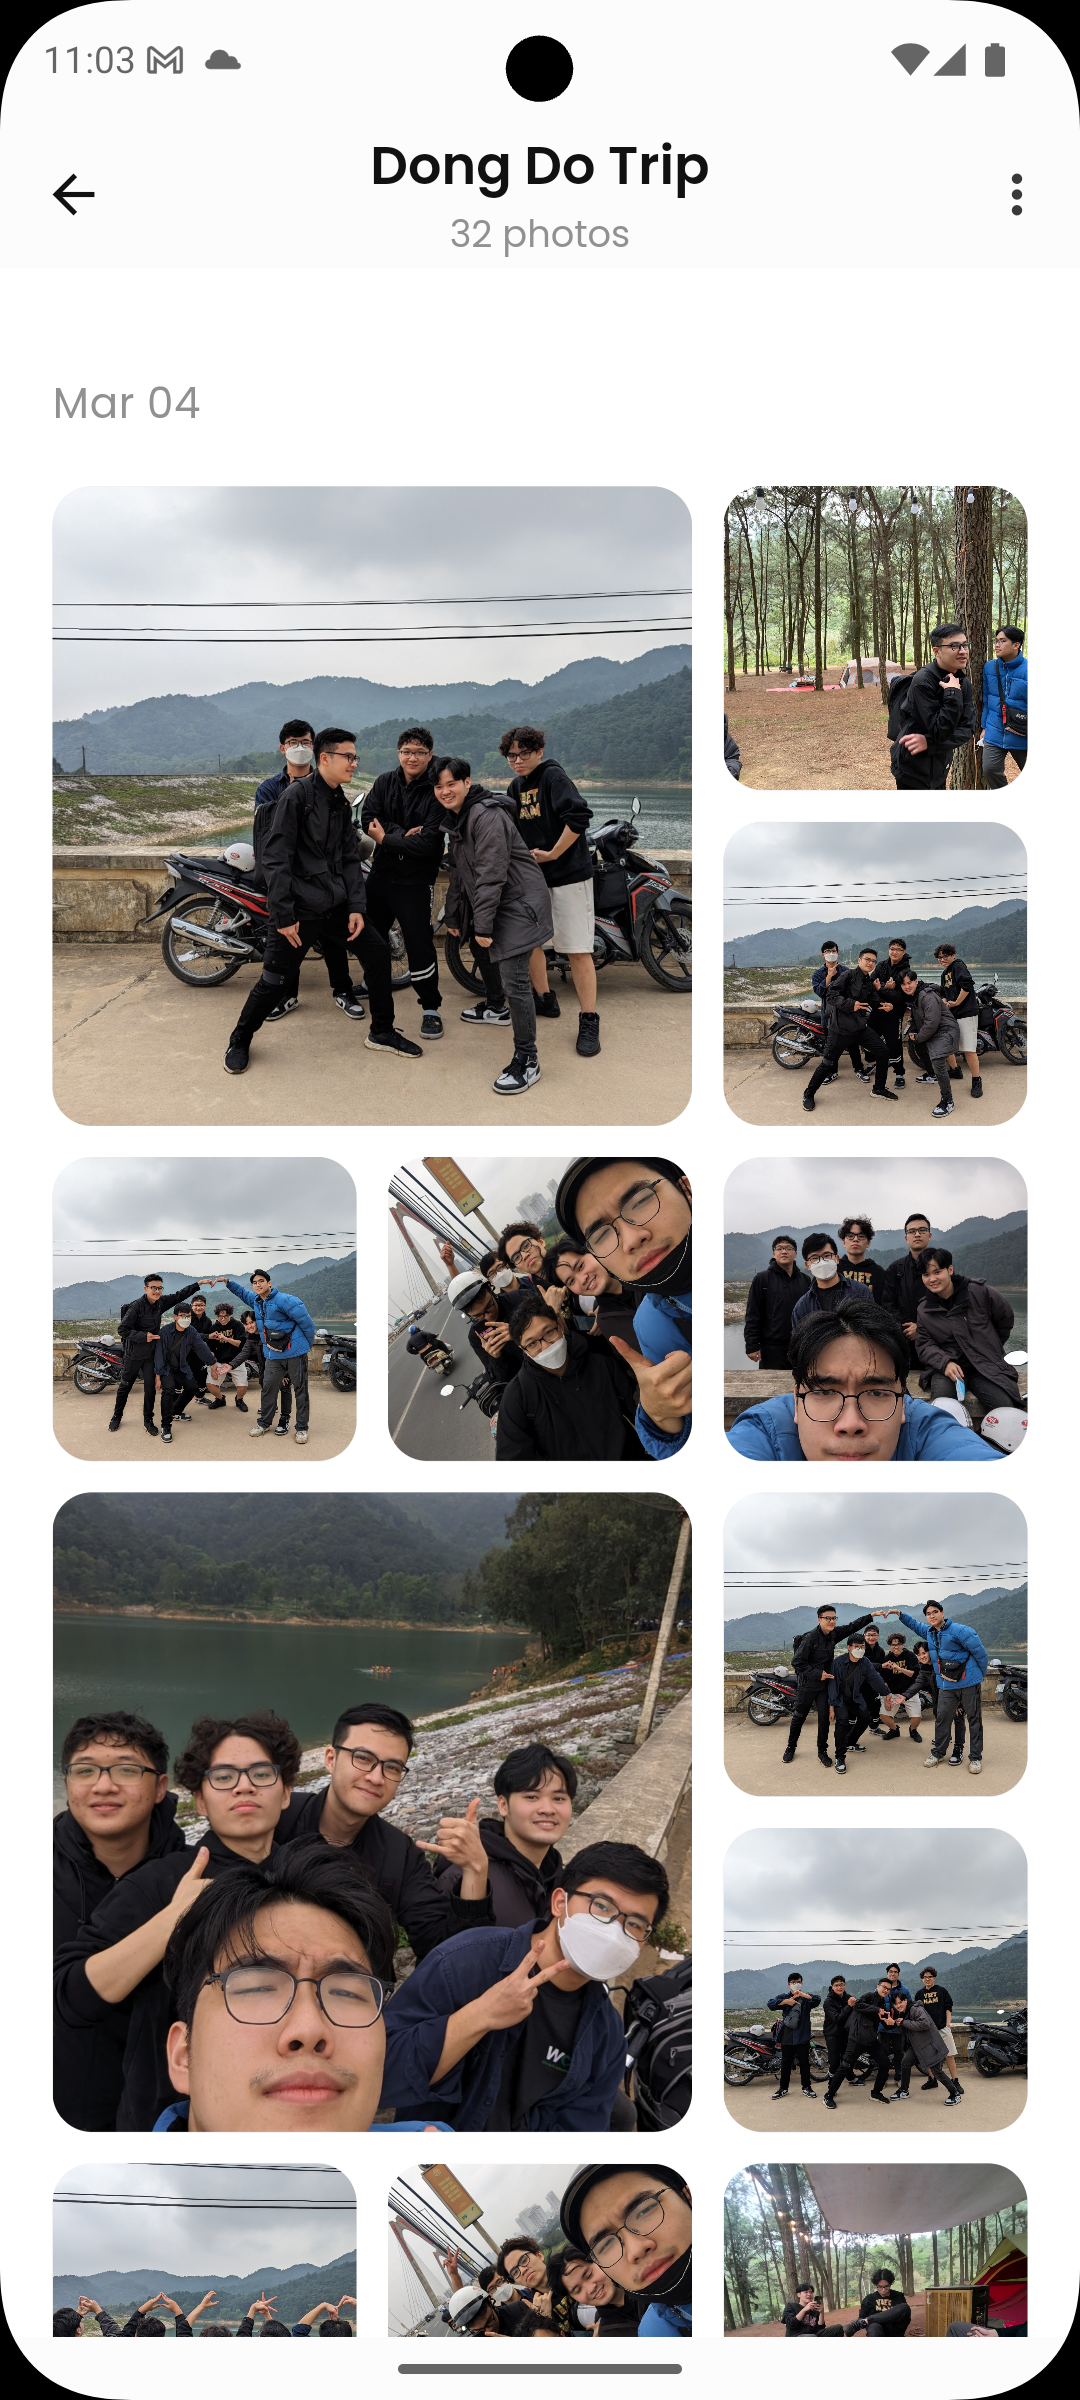
\includegraphics[width=1\linewidth]{figures/c4/4-2/album_2.png} 
        \caption{Danh sách ảnh trong album}
    \end{subfigure}
    \begin{subfigure}{0.32\textwidth}
        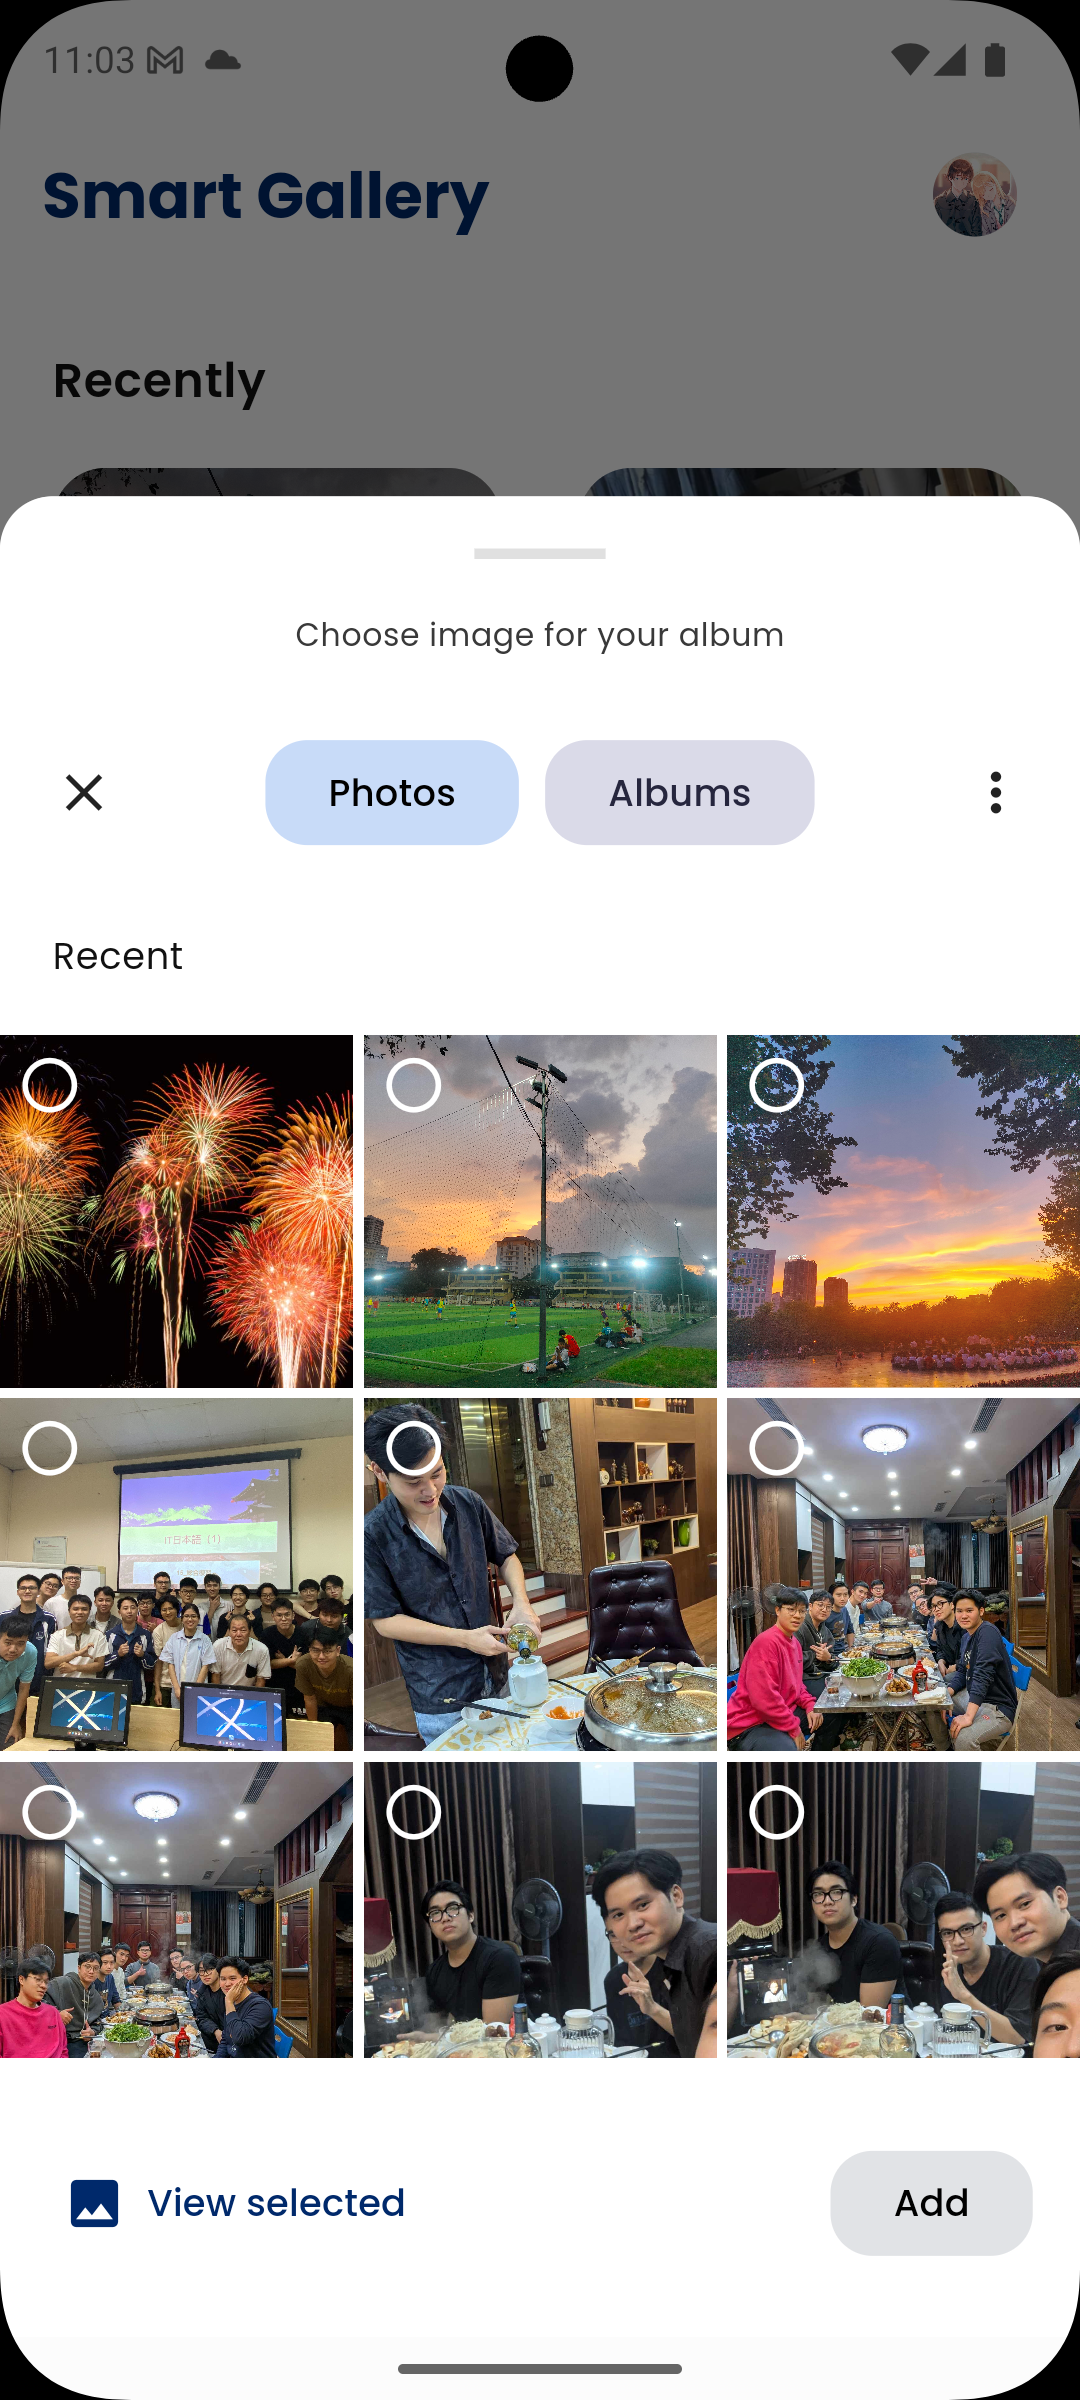
\includegraphics[width=1\linewidth]{figures/c4/4-2/create_album.png}
        \caption{Tạo album}
    \end{subfigure}
    \caption{Giao diện album ảnh.}
    \label{fig:album}
\end{figure}

% Hệ thống cung cấp giao diện tạo album với các ảnh người dùng đã tải lên hệ thống như Hình \ref{fig:create-album}

% \begin{figure}[H]
%     \centering  
%     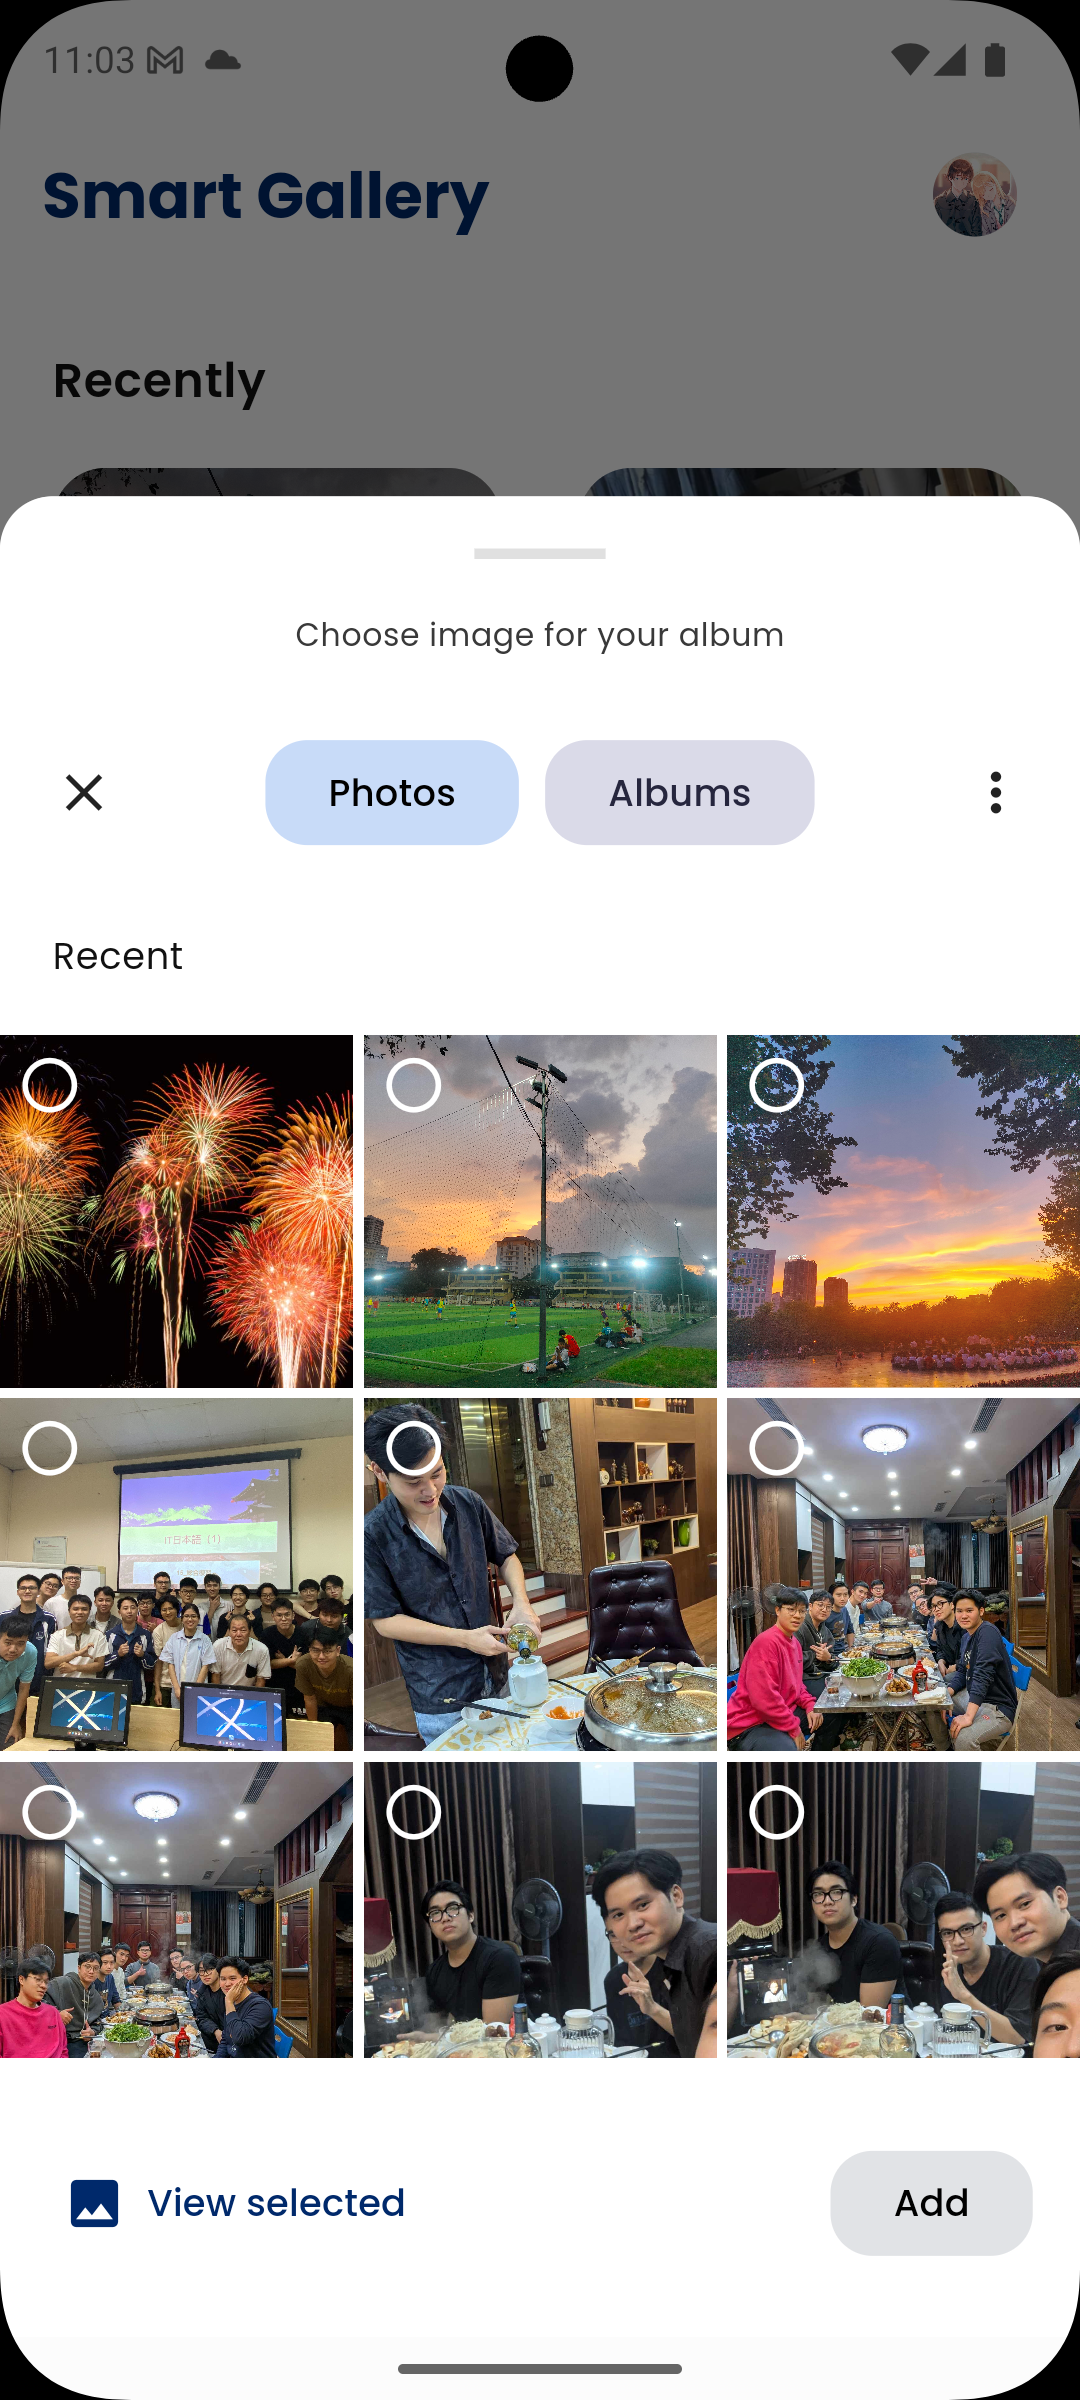
\includegraphics[width=0.5\textwidth]{figures/c4/4-2/create_album.png}
%     \caption{Giao diện tạo album.}
%     \label{fig:create-album}
% \end{figure}

\subsection{Giao diện khám phá}

Hệ thống cung cấp chức năng khám phá cho phép người dùng khám phá những khía cạnh khác nhau của ảnh như nhãn, vị trí chụp, khuôn mặt trong bức ảnh.

Các nhãn được phân loại từ các ảnh người dùng tải lên sẽ được hệ thống phân loại, nhóm thành các nhóm khác nhau dựa theo địa điểm, hành động và sự kiện trong ảnh như Hình \ref{fig:explore_label}.

\begin{figure}[H]
    \centering
    \begin{subfigure}{0.32\textwidth}
        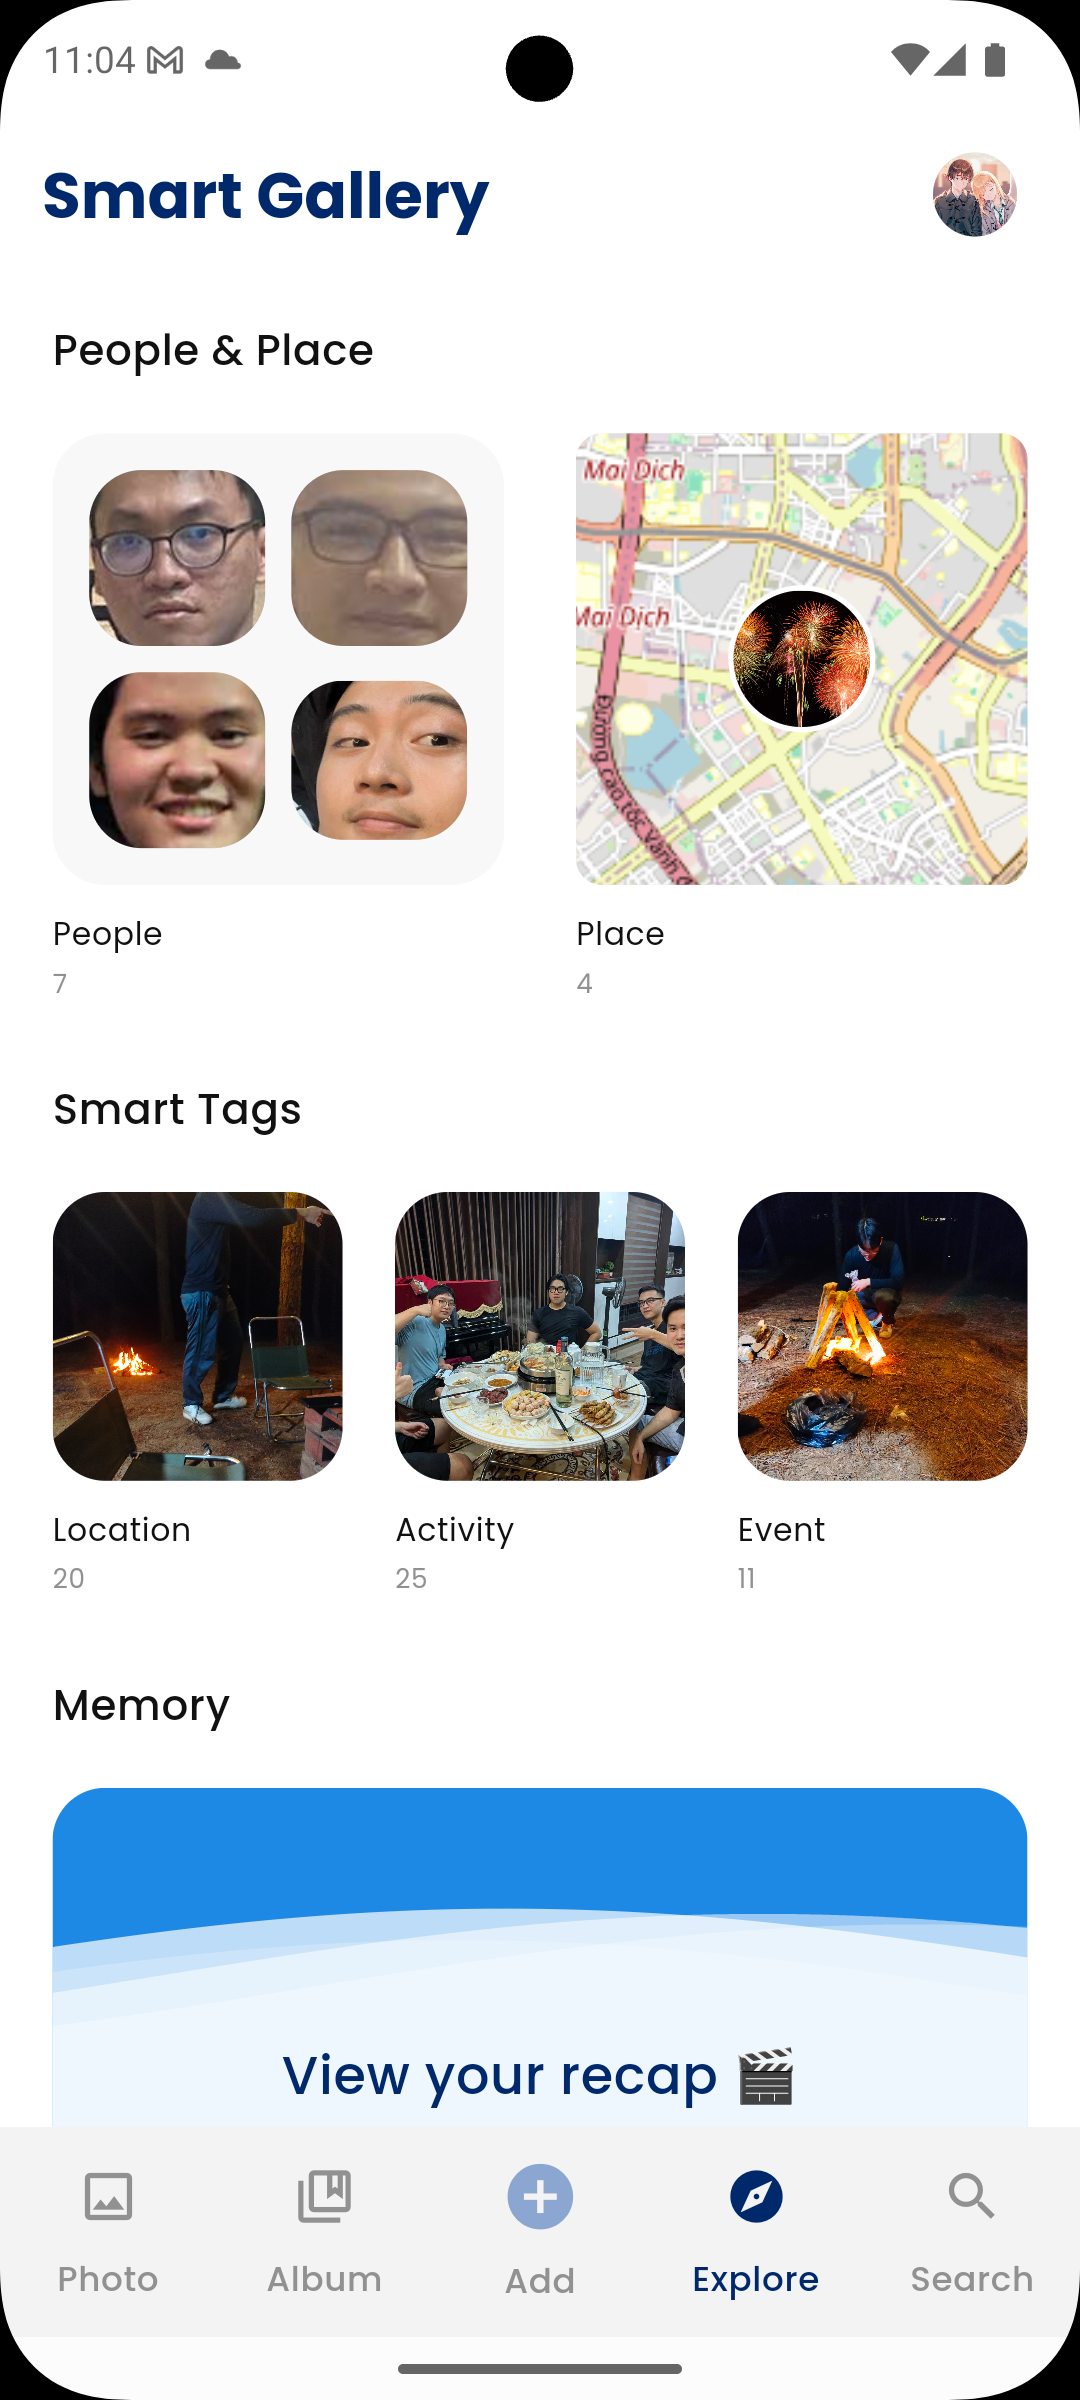
\includegraphics[width=1\linewidth]{figures/c4/4-2/explore_1.png} 
        \caption{Trang chủ}
    \end{subfigure}
    \hfill
    \begin{subfigure}{0.32\textwidth}
        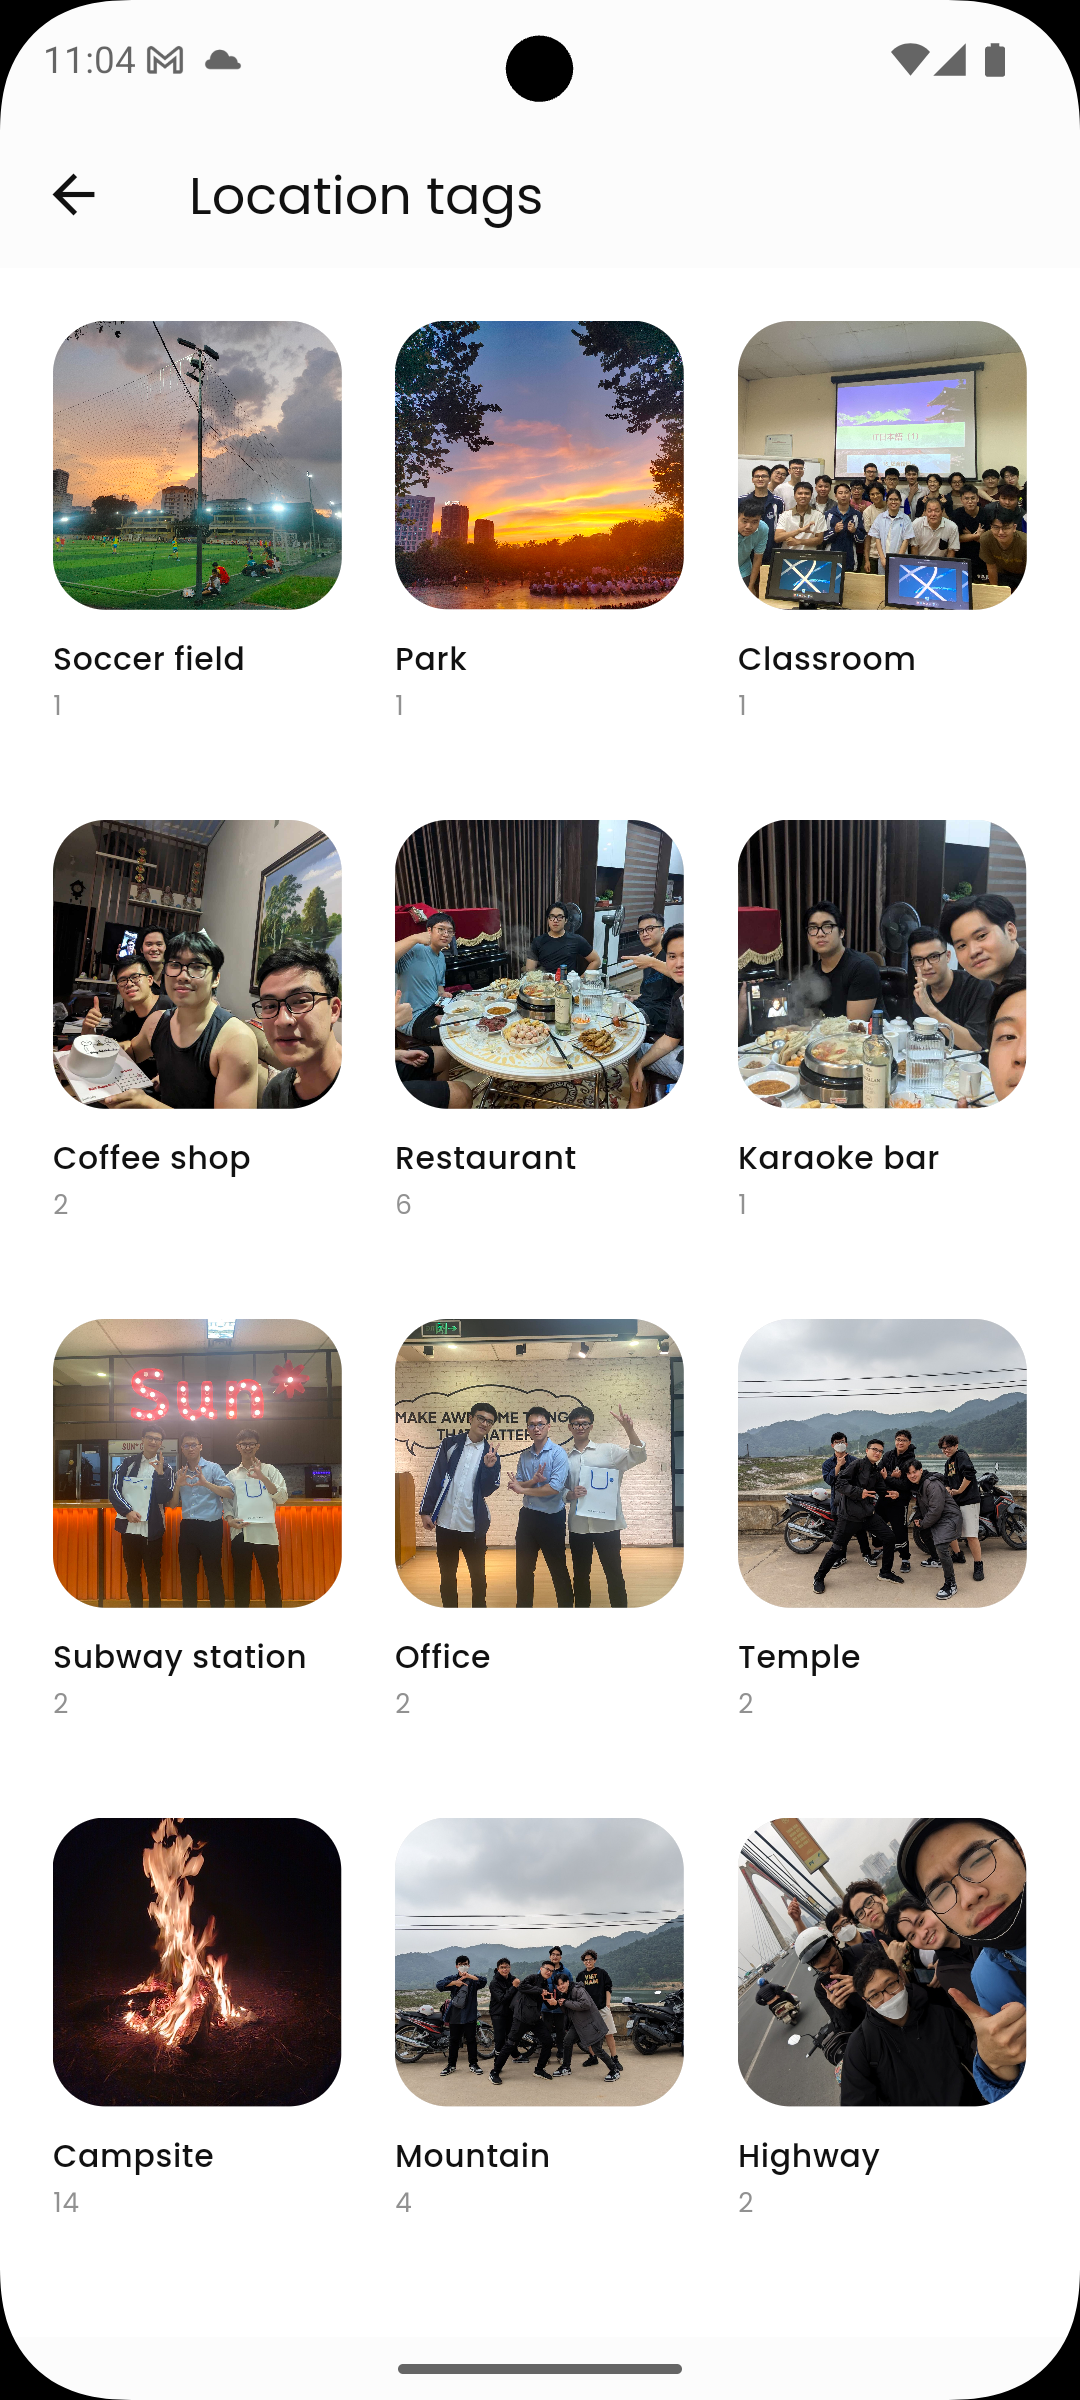
\includegraphics[width=1\linewidth]{figures/c4/4-2/explore_2.png} 
        \caption{Danh sách nhãn ảnh}
    \end{subfigure}
    \hfill
    \begin{subfigure}{0.32\textwidth}
        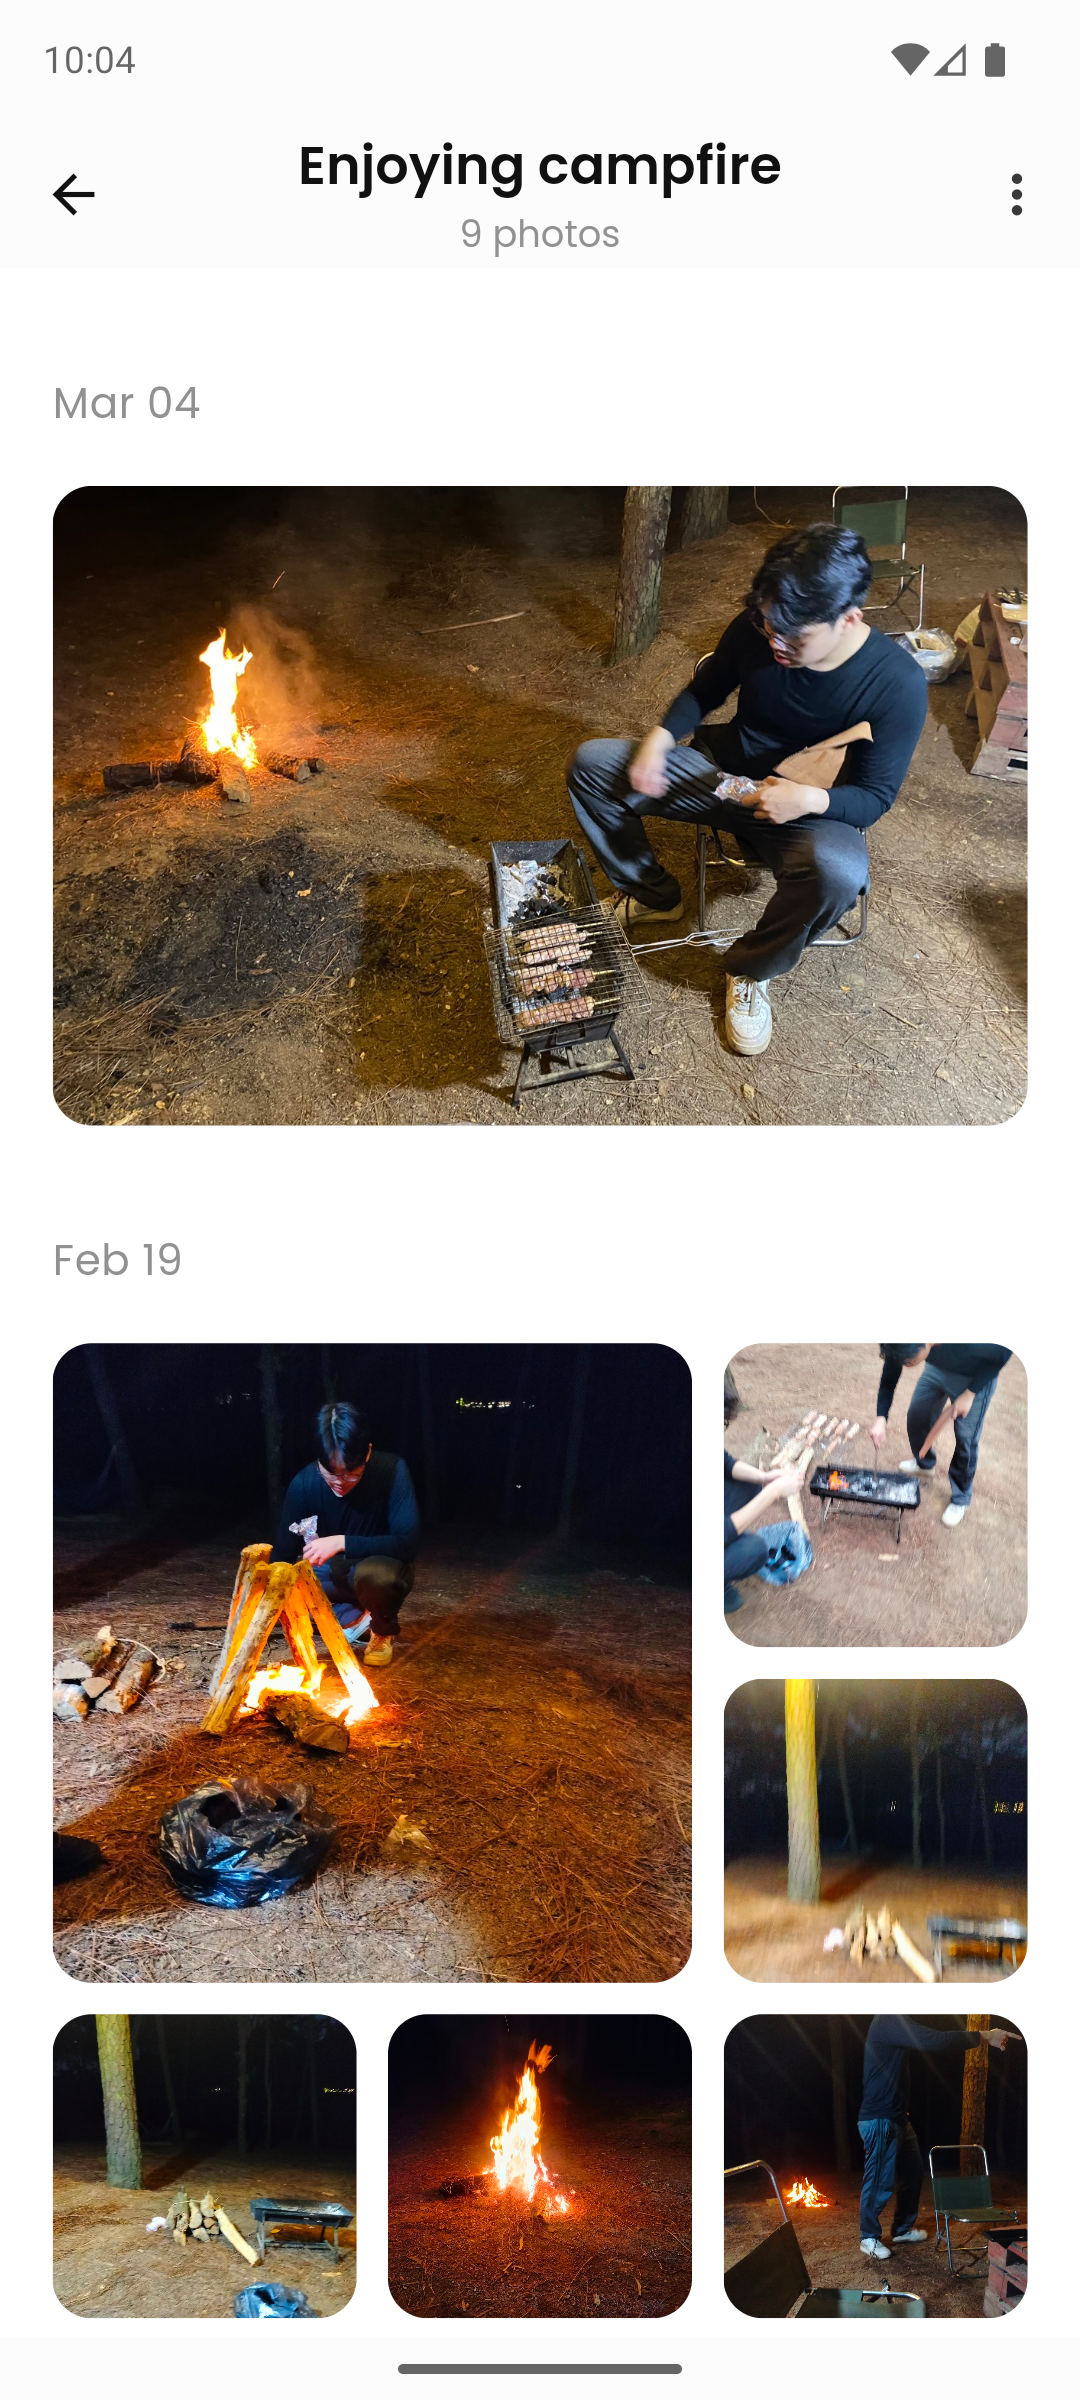
\includegraphics[width=1\linewidth]{figures/c4/4-2/explore_3.png} 
        \caption{Xem chi tiết nhãn ảnh}
    \end{subfigure}
    \caption{Giao diện khám phá.}
    \label{fig:explore_label}
\end{figure}

Hệ thống cũng cung cấp tính năng quản lý ảnh theo địa điểm. Người dùng có thể xem, chỉnh sửa các vị trí cho ảnh, đồng thời được hệ thống phân nhóm các ảnh theo vị trí chụp như Hình \ref{fig:explore_location}.

\begin{figure}[H]
    \centering
    \begin{subfigure}{0.32\textwidth}
        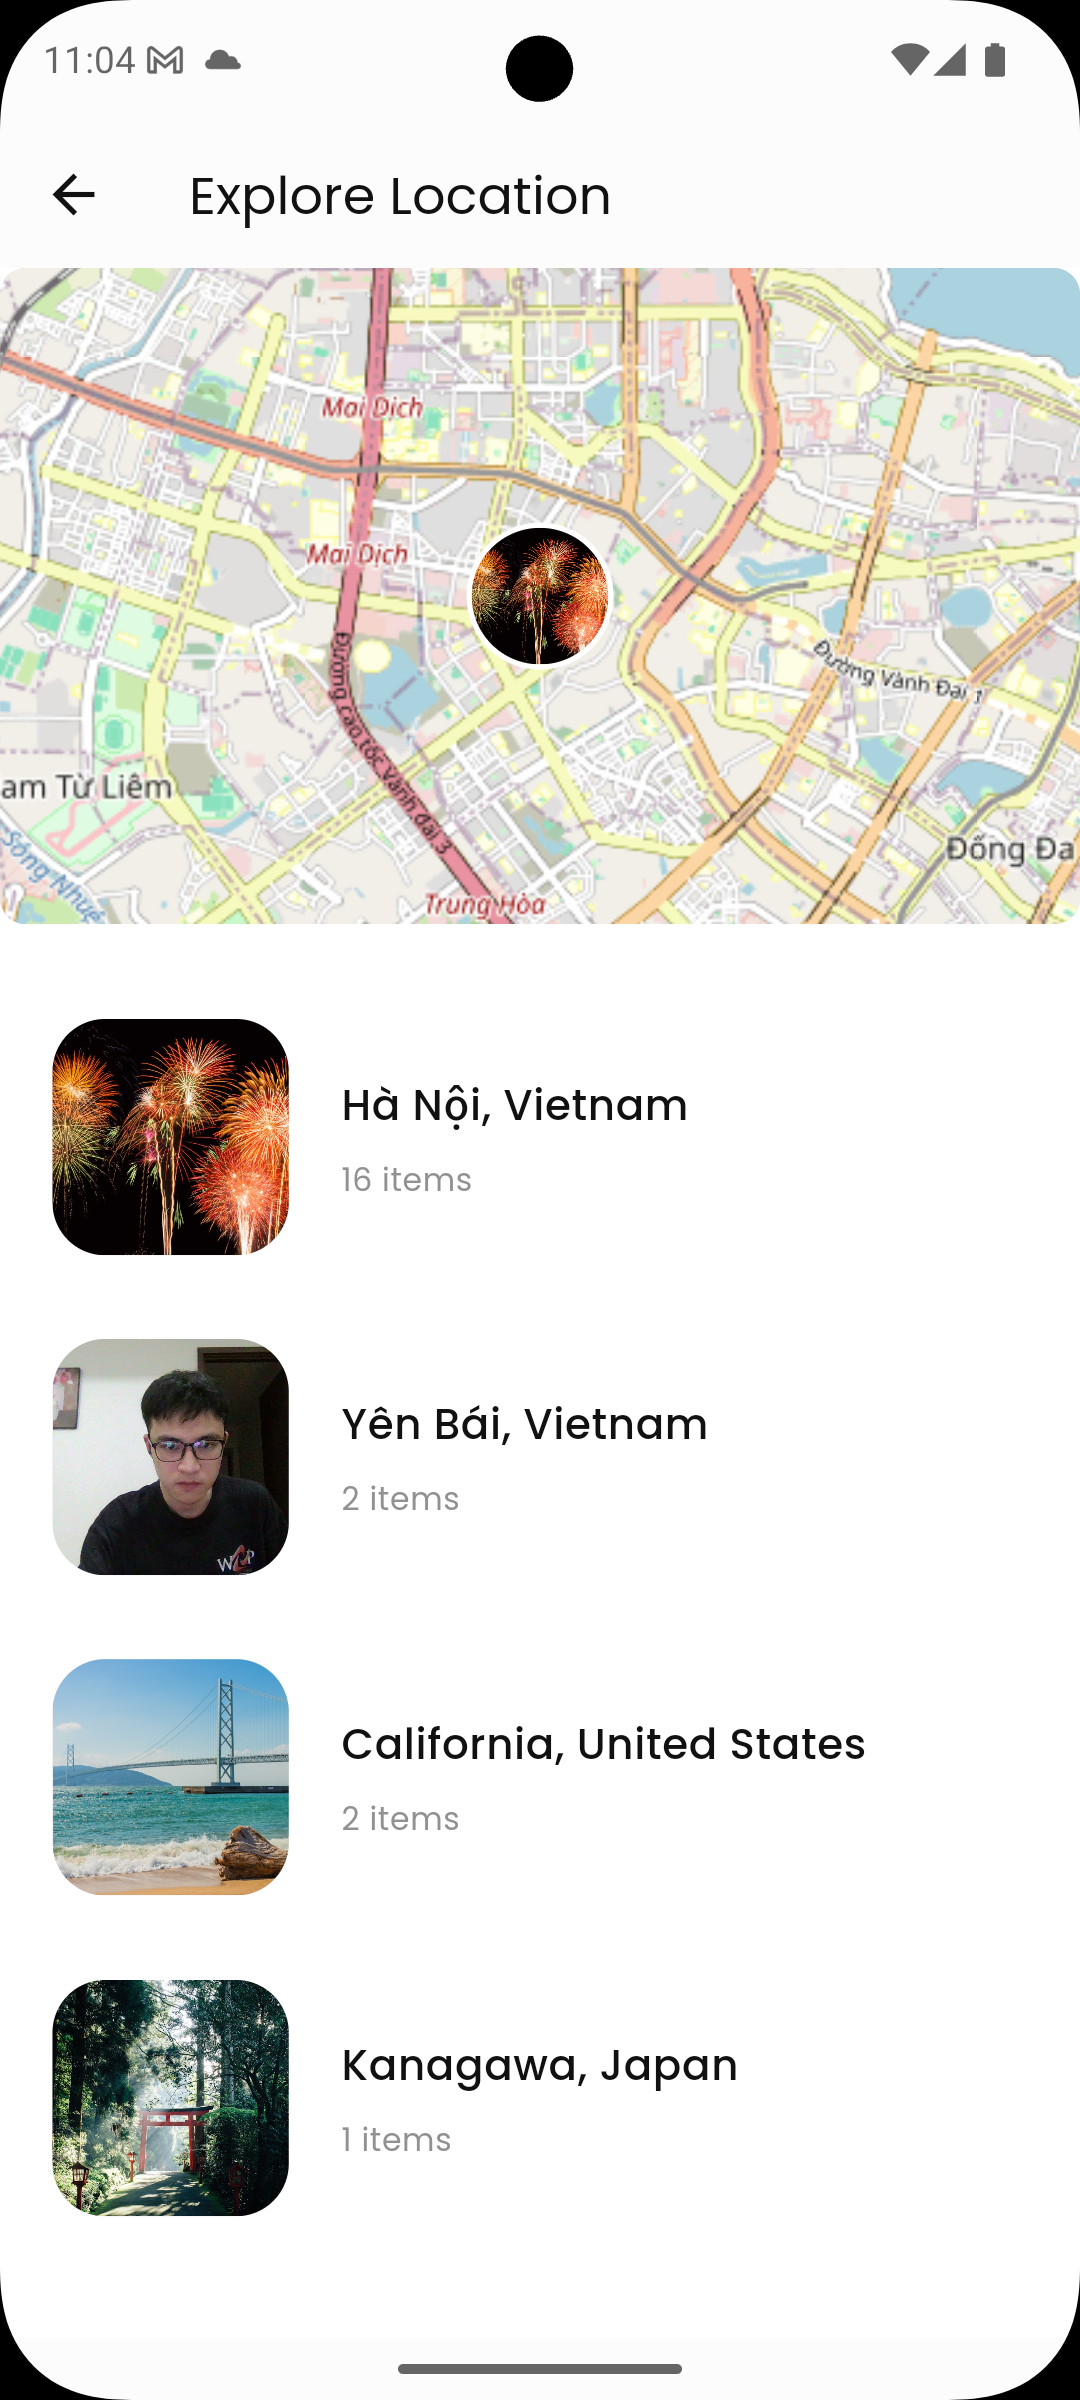
\includegraphics[width=1\linewidth]{figures/c4/4-2/location_1.png} 
        \caption{Nhóm ảnh theo vị trí}
    \end{subfigure}
    \hfill
    \begin{subfigure}{0.32\textwidth}
        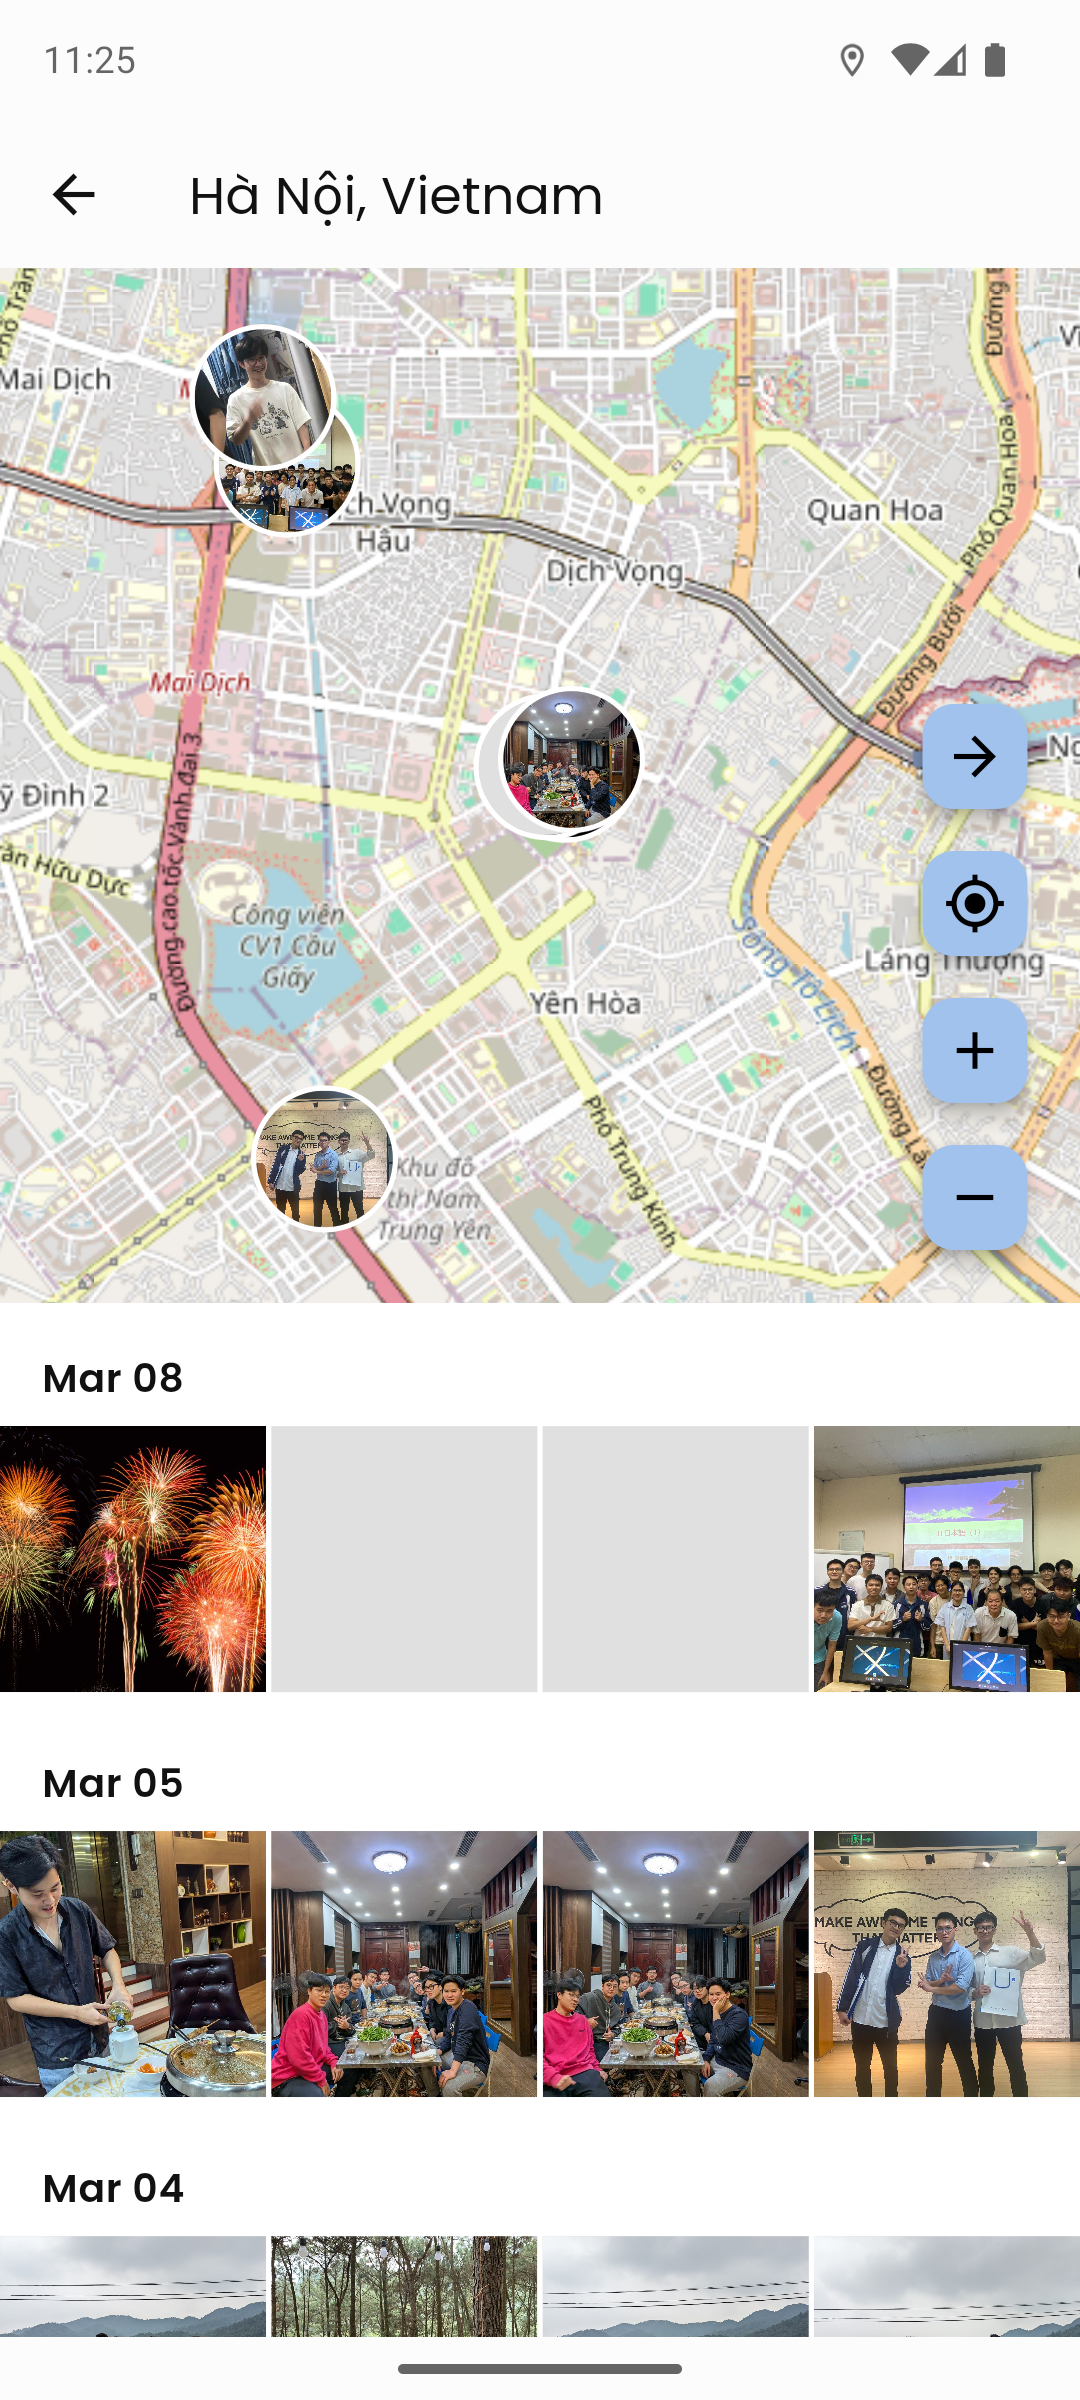
\includegraphics[width=1\linewidth]{figures/c4/4-2/location_2.png} 
        \caption{Xem ảnh theo vị trí}
    \end{subfigure}
    \hfill
    \begin{subfigure}{0.32\textwidth}
        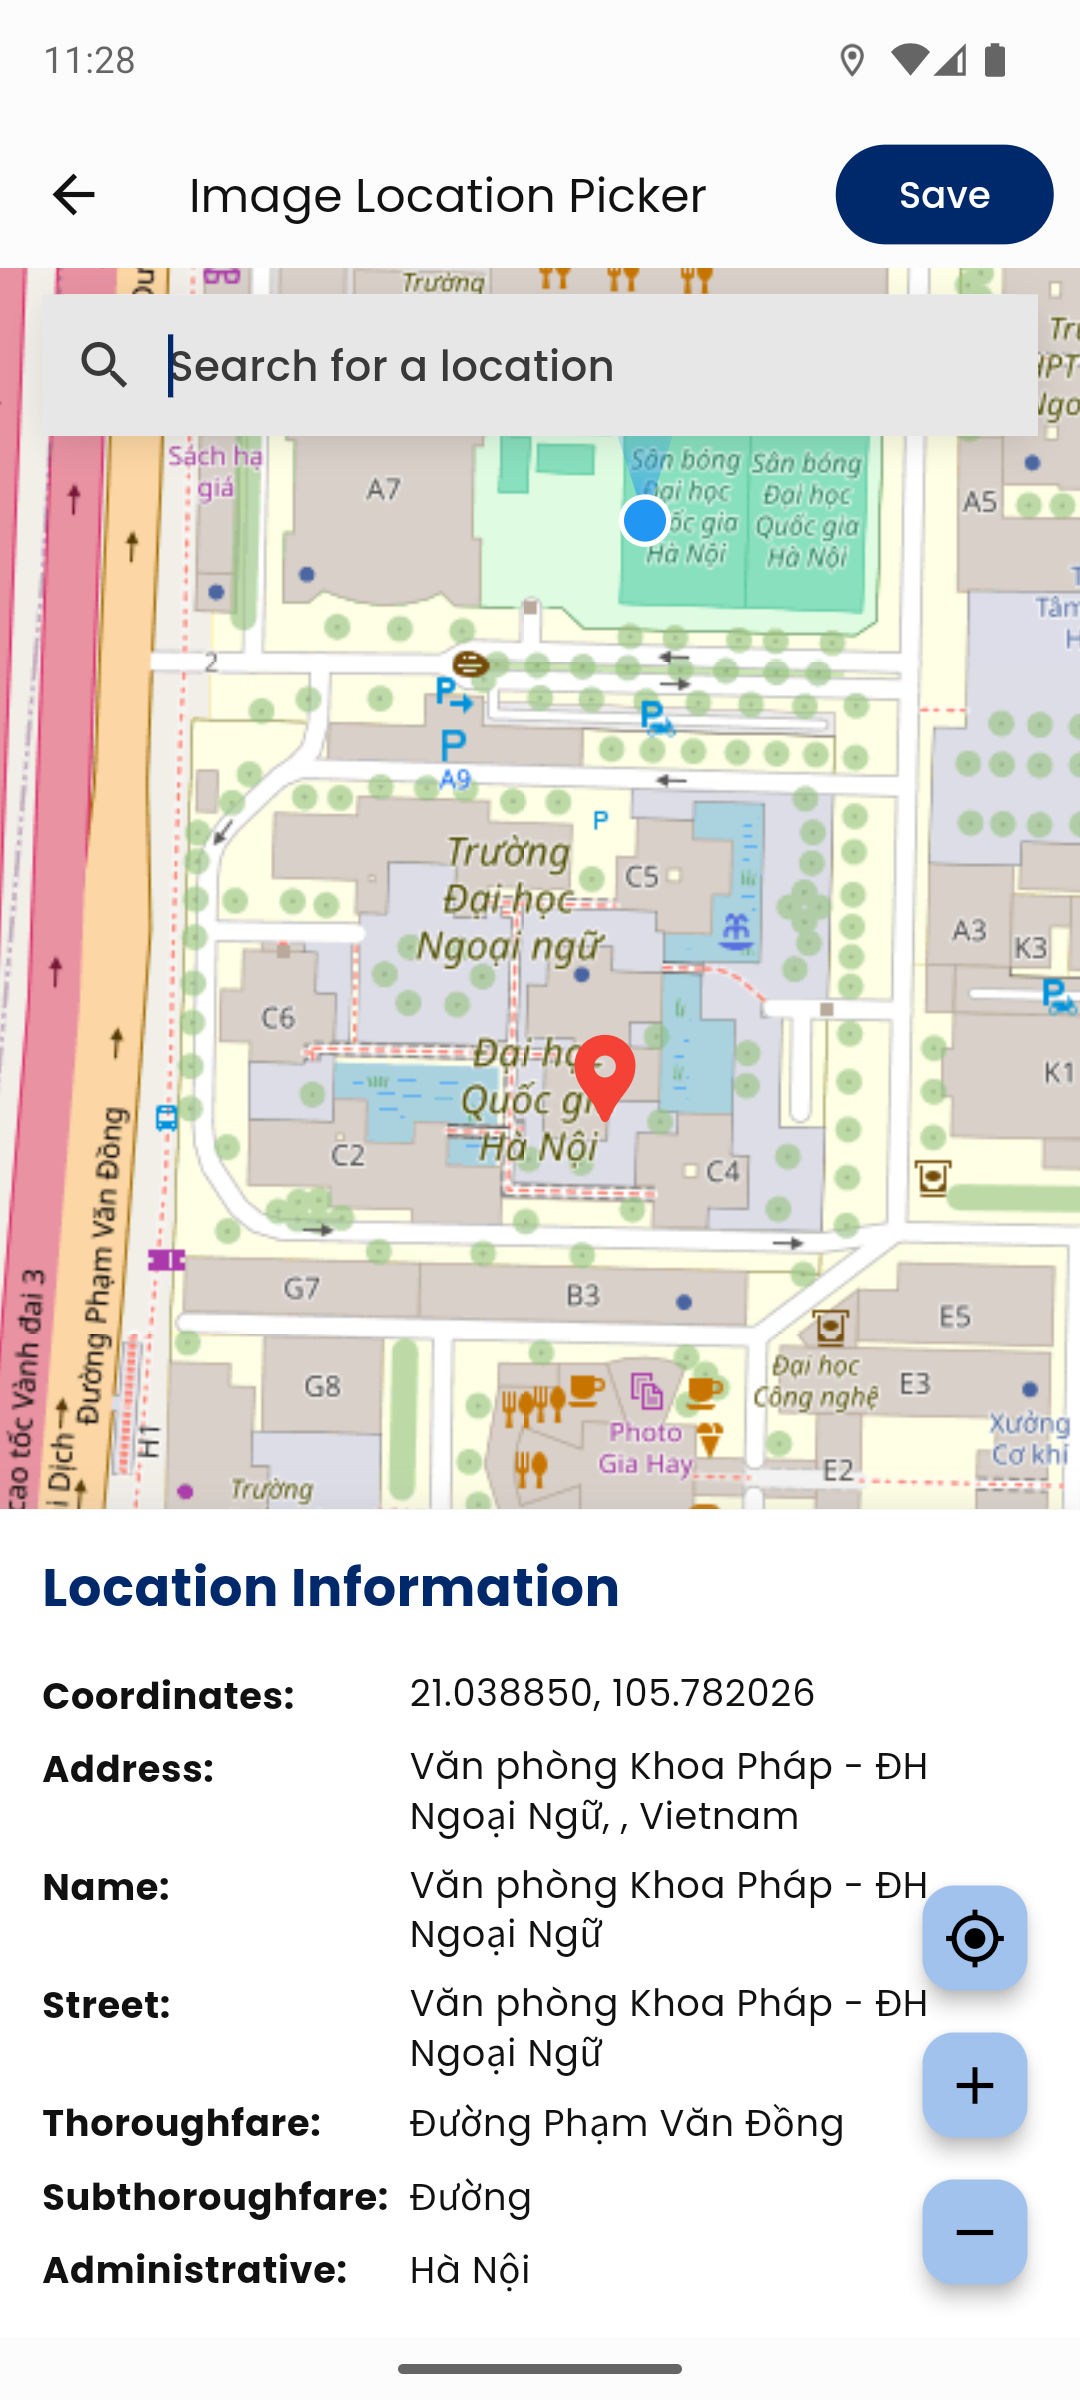
\includegraphics[width=1\linewidth]{figures/c4/4-2/location_3.png} 
        \caption{Thêm vị trí cho ảnh}
    \end{subfigure}
    \caption{Giao diện quản lý vị trí ảnh.}
    \label{fig:explore_location}
\end{figure}

Ngoài ra hệ thống cũng cung cấp tính năng nhận diện khuôn mặt trong ảnh. Người dùng có thể xem, chỉnh sửa các khuôn mặt trong ảnh, đồng thời được hệ thống phân nhóm các ảnh theo khuôn mặt như Hình \ref{fig:explore_face}.

\begin{figure}[H]
    \centering
    \begin{subfigure}{0.32\textwidth}
        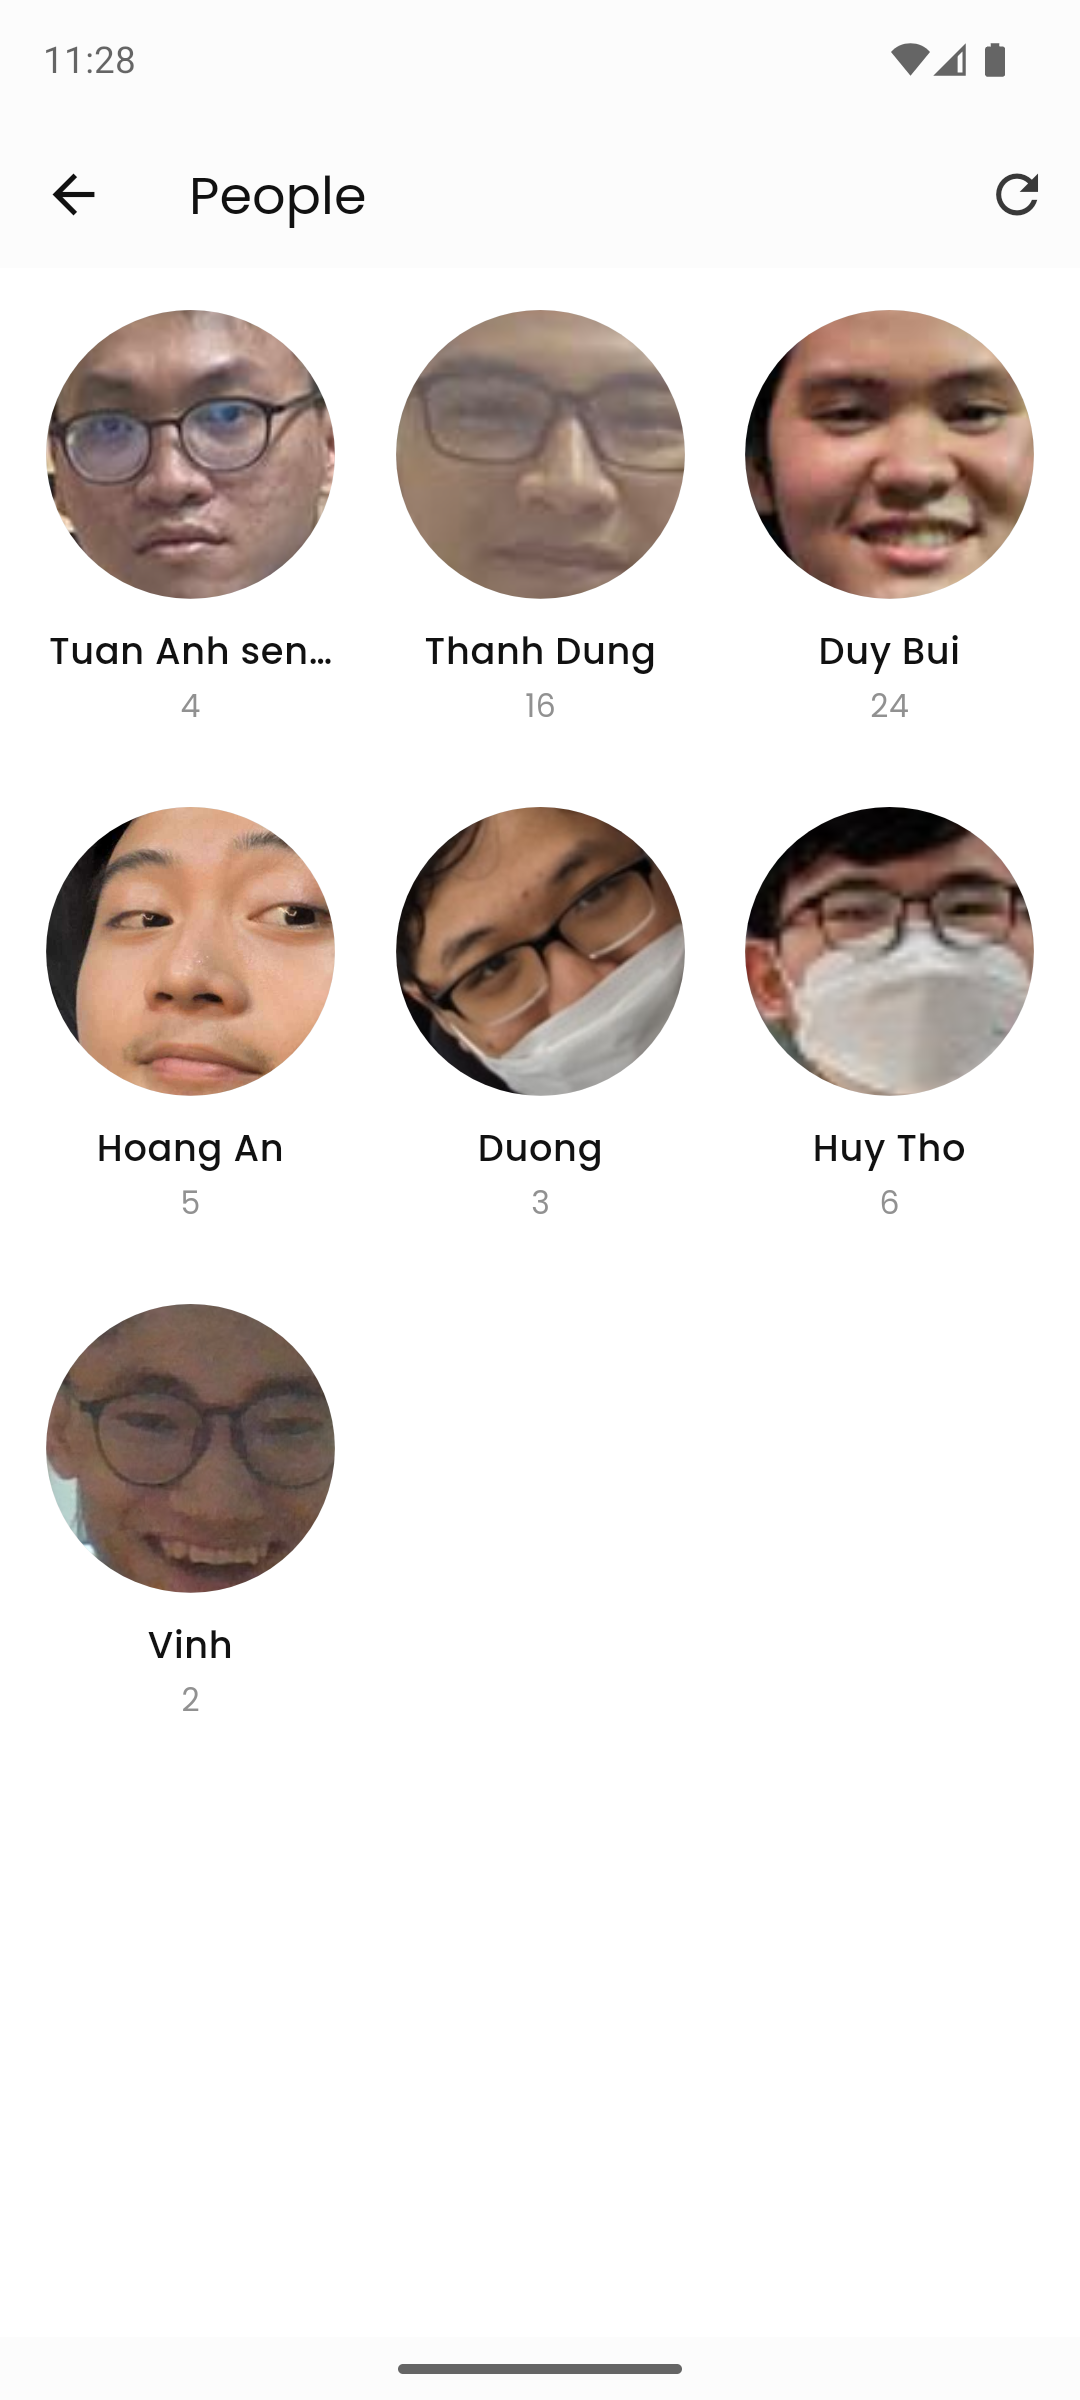
\includegraphics[width=1\linewidth]{figures/c4/4-2/face_1.png} 
        \caption{Danh sách khuôn mặt}
    \end{subfigure}
    \hfill
    \begin{subfigure}{0.32\textwidth}
        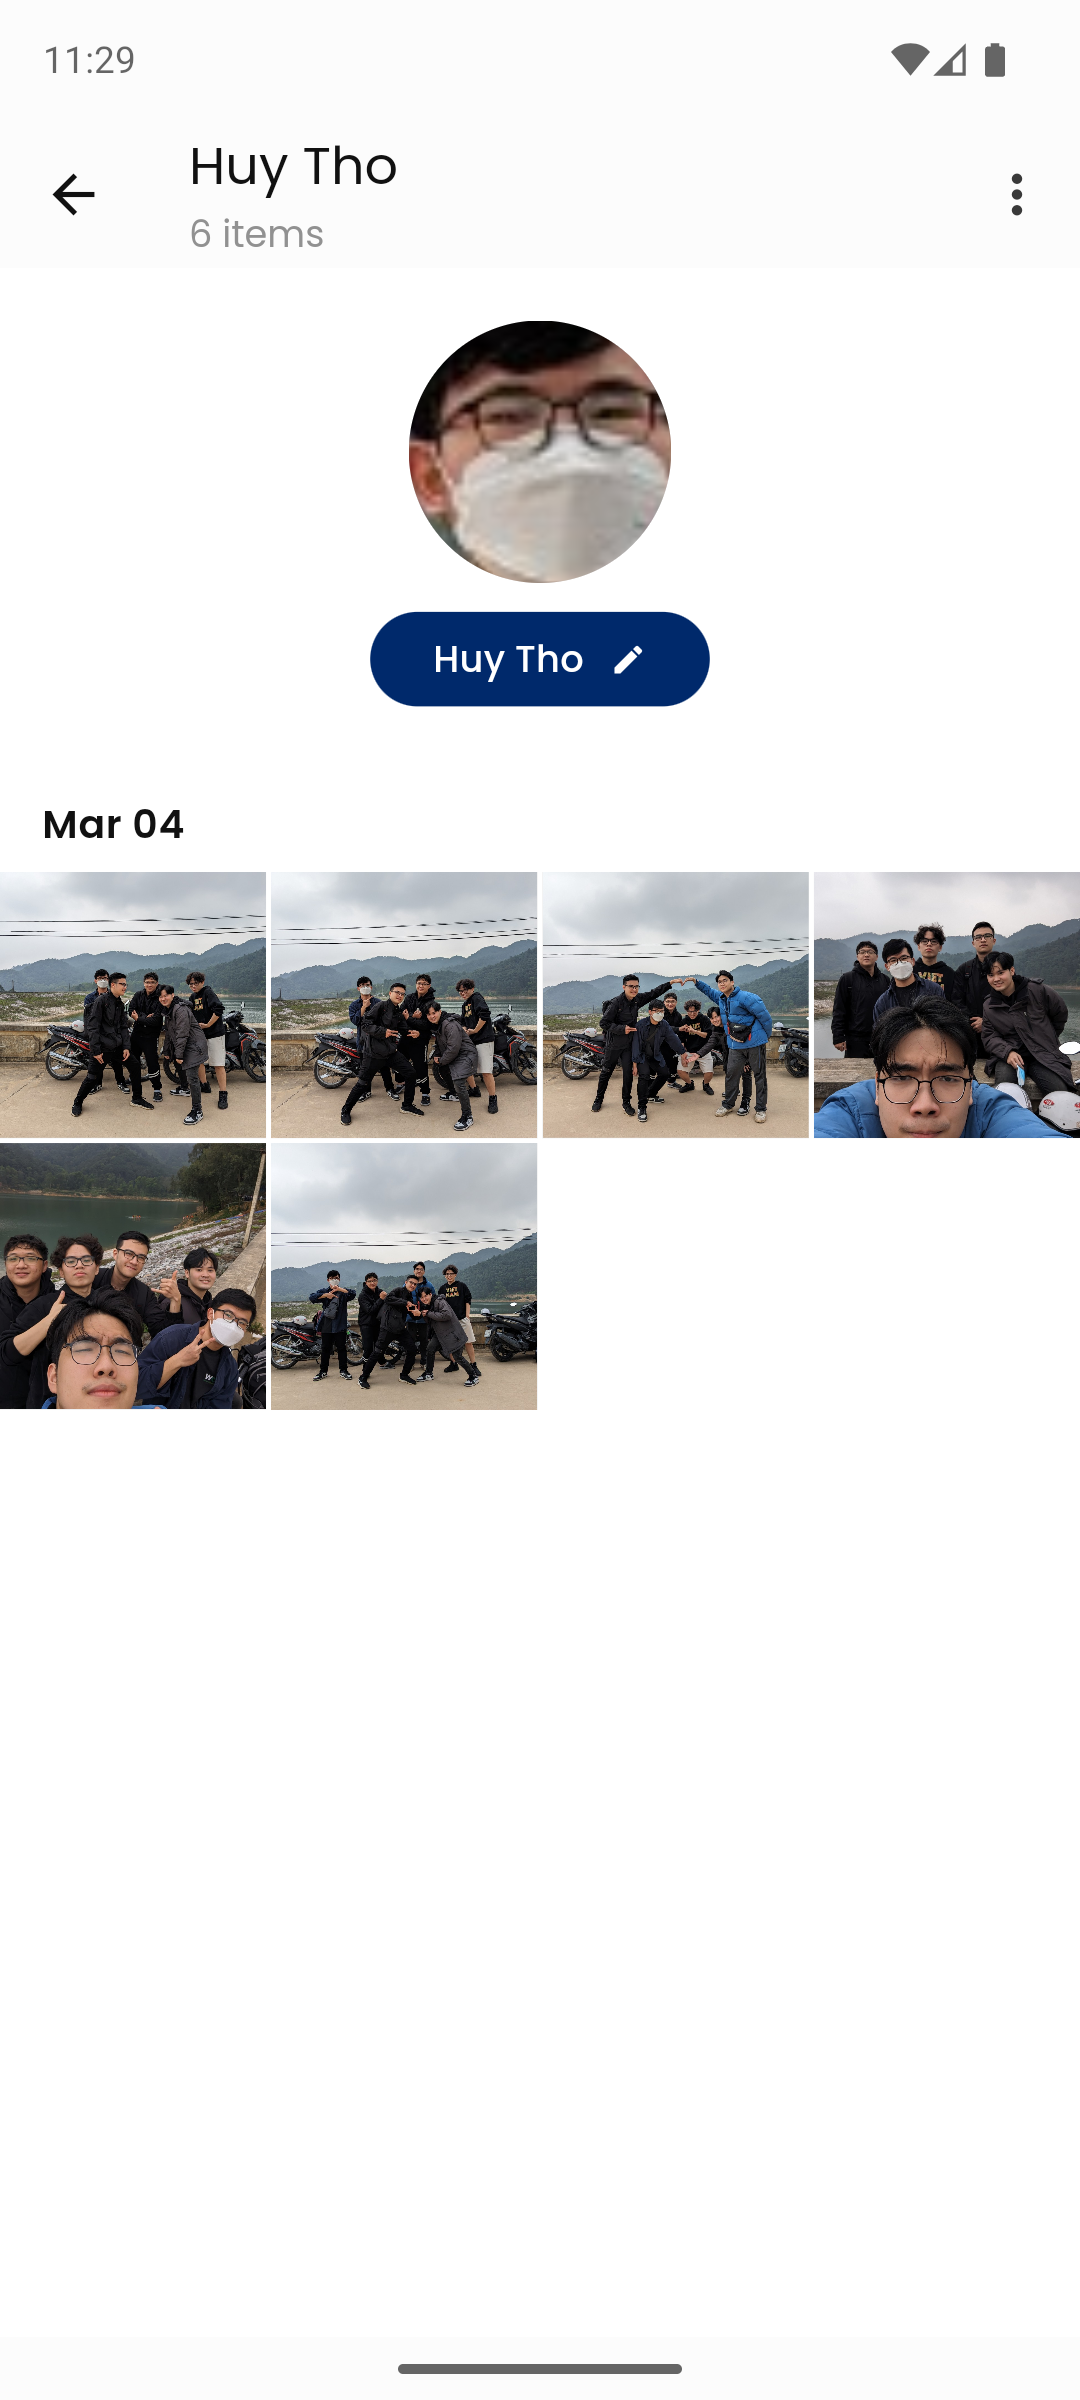
\includegraphics[width=1\linewidth]{figures/c4/4-2/face_2.png} 
        \caption{Xem ảnh theo khuôn mặt}
    \end{subfigure}
    \hfill
    \begin{subfigure}{0.32\textwidth}
        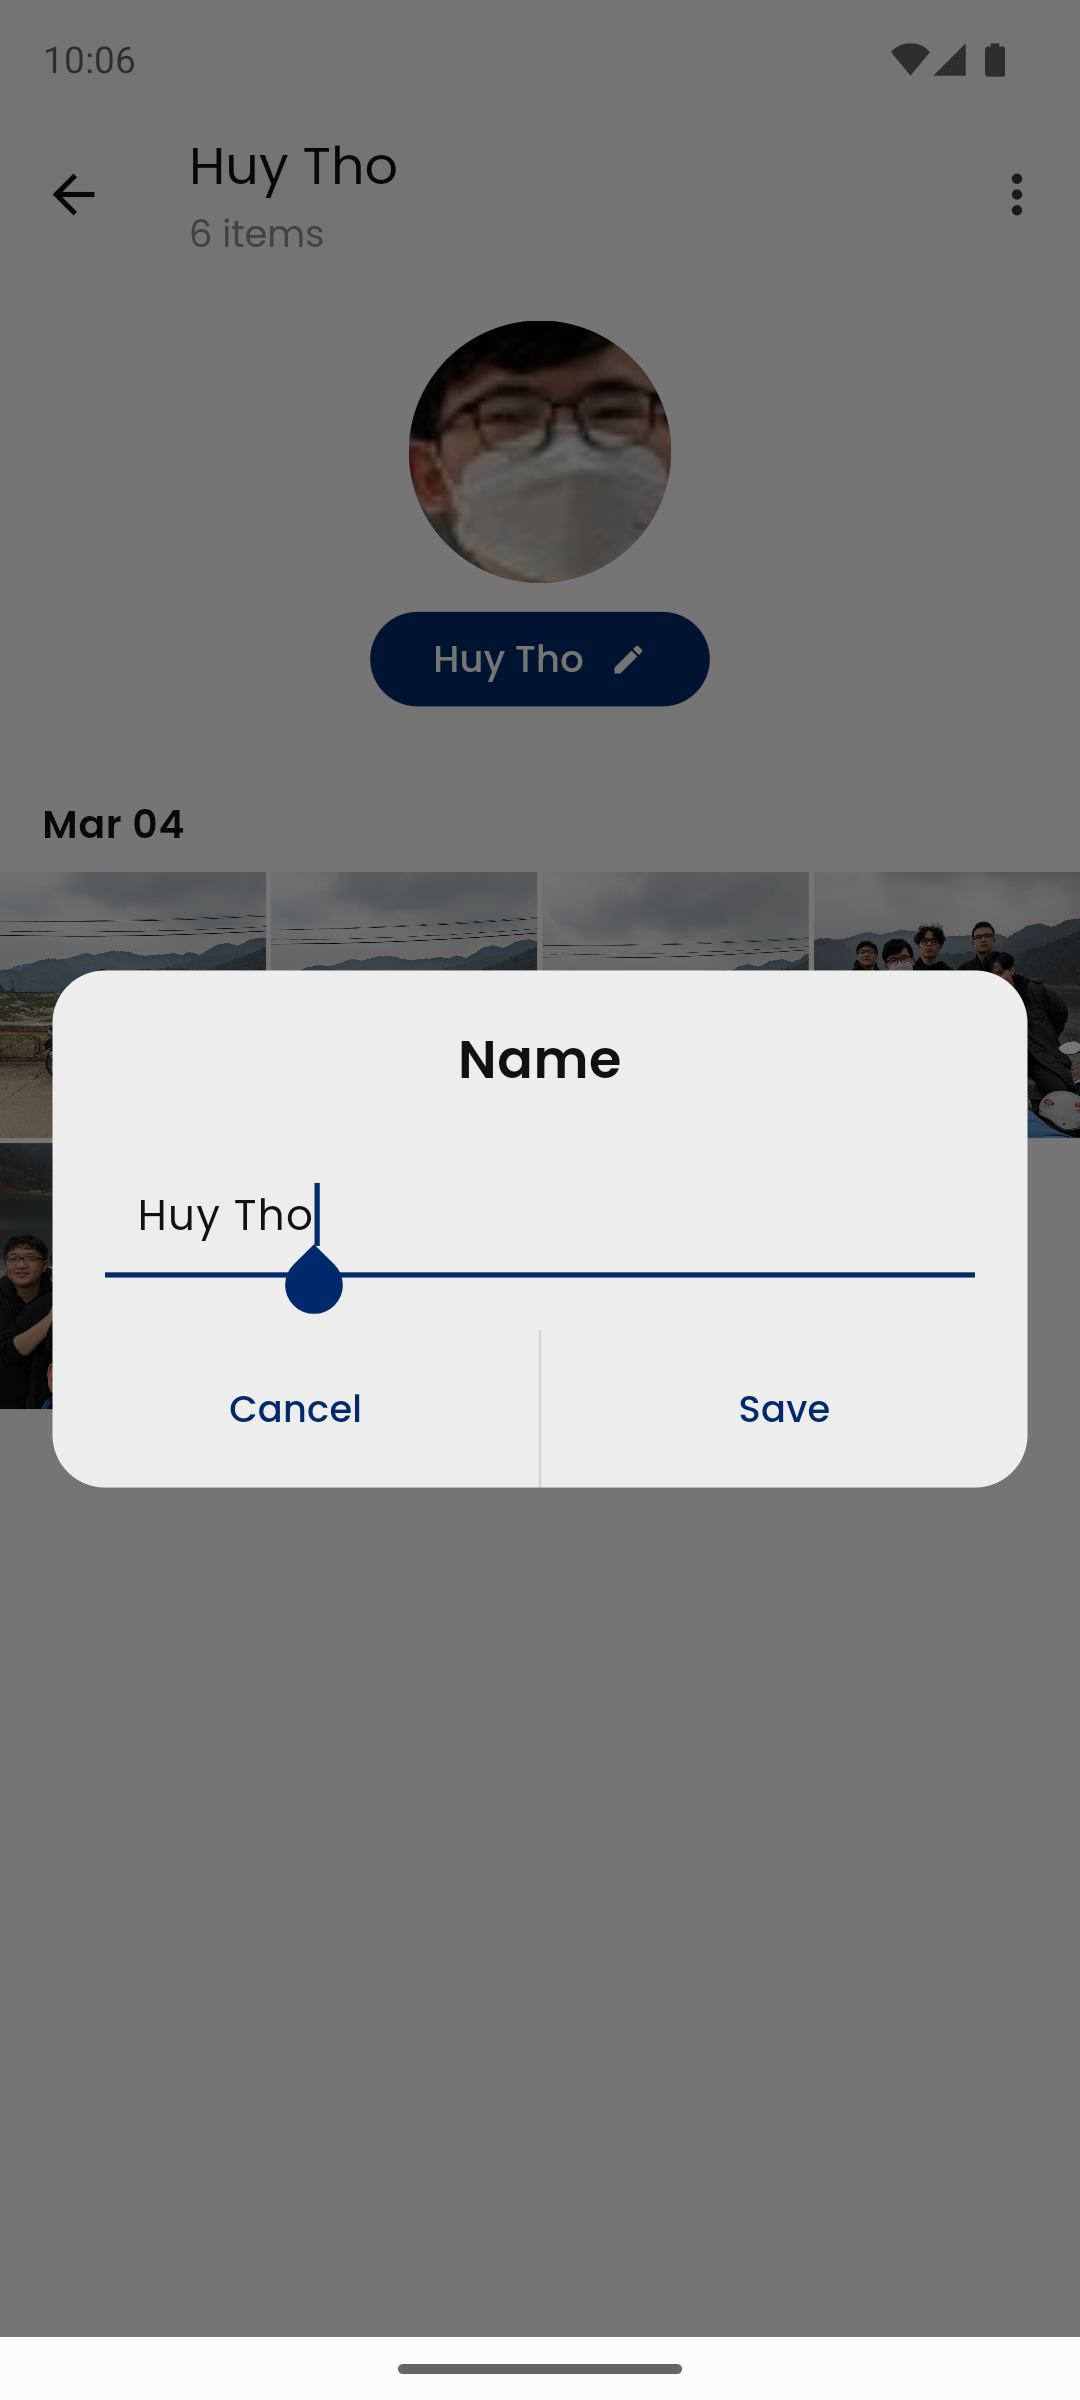
\includegraphics[width=1\linewidth]{figures/c4/4-2/face_3.png} 
        \caption{Chỉnh sửa tên}
    \end{subfigure}
    \caption{Giao diện quản lý khuôn mặt.}
    \label{fig:explore_face}
\end{figure}

\subsection{Quản lý video recap}

Người dùng có thể quản lý video recap của mình thông qua chức năng này. Hệ thống cho phép người dùng xem và theo dõi tiến độ tạo video của mình theo thời gian thực như Hình \ref{fig:video_recap}.

\begin{figure}[H]
    \centering
    \begin{subfigure}{0.32\textwidth}
        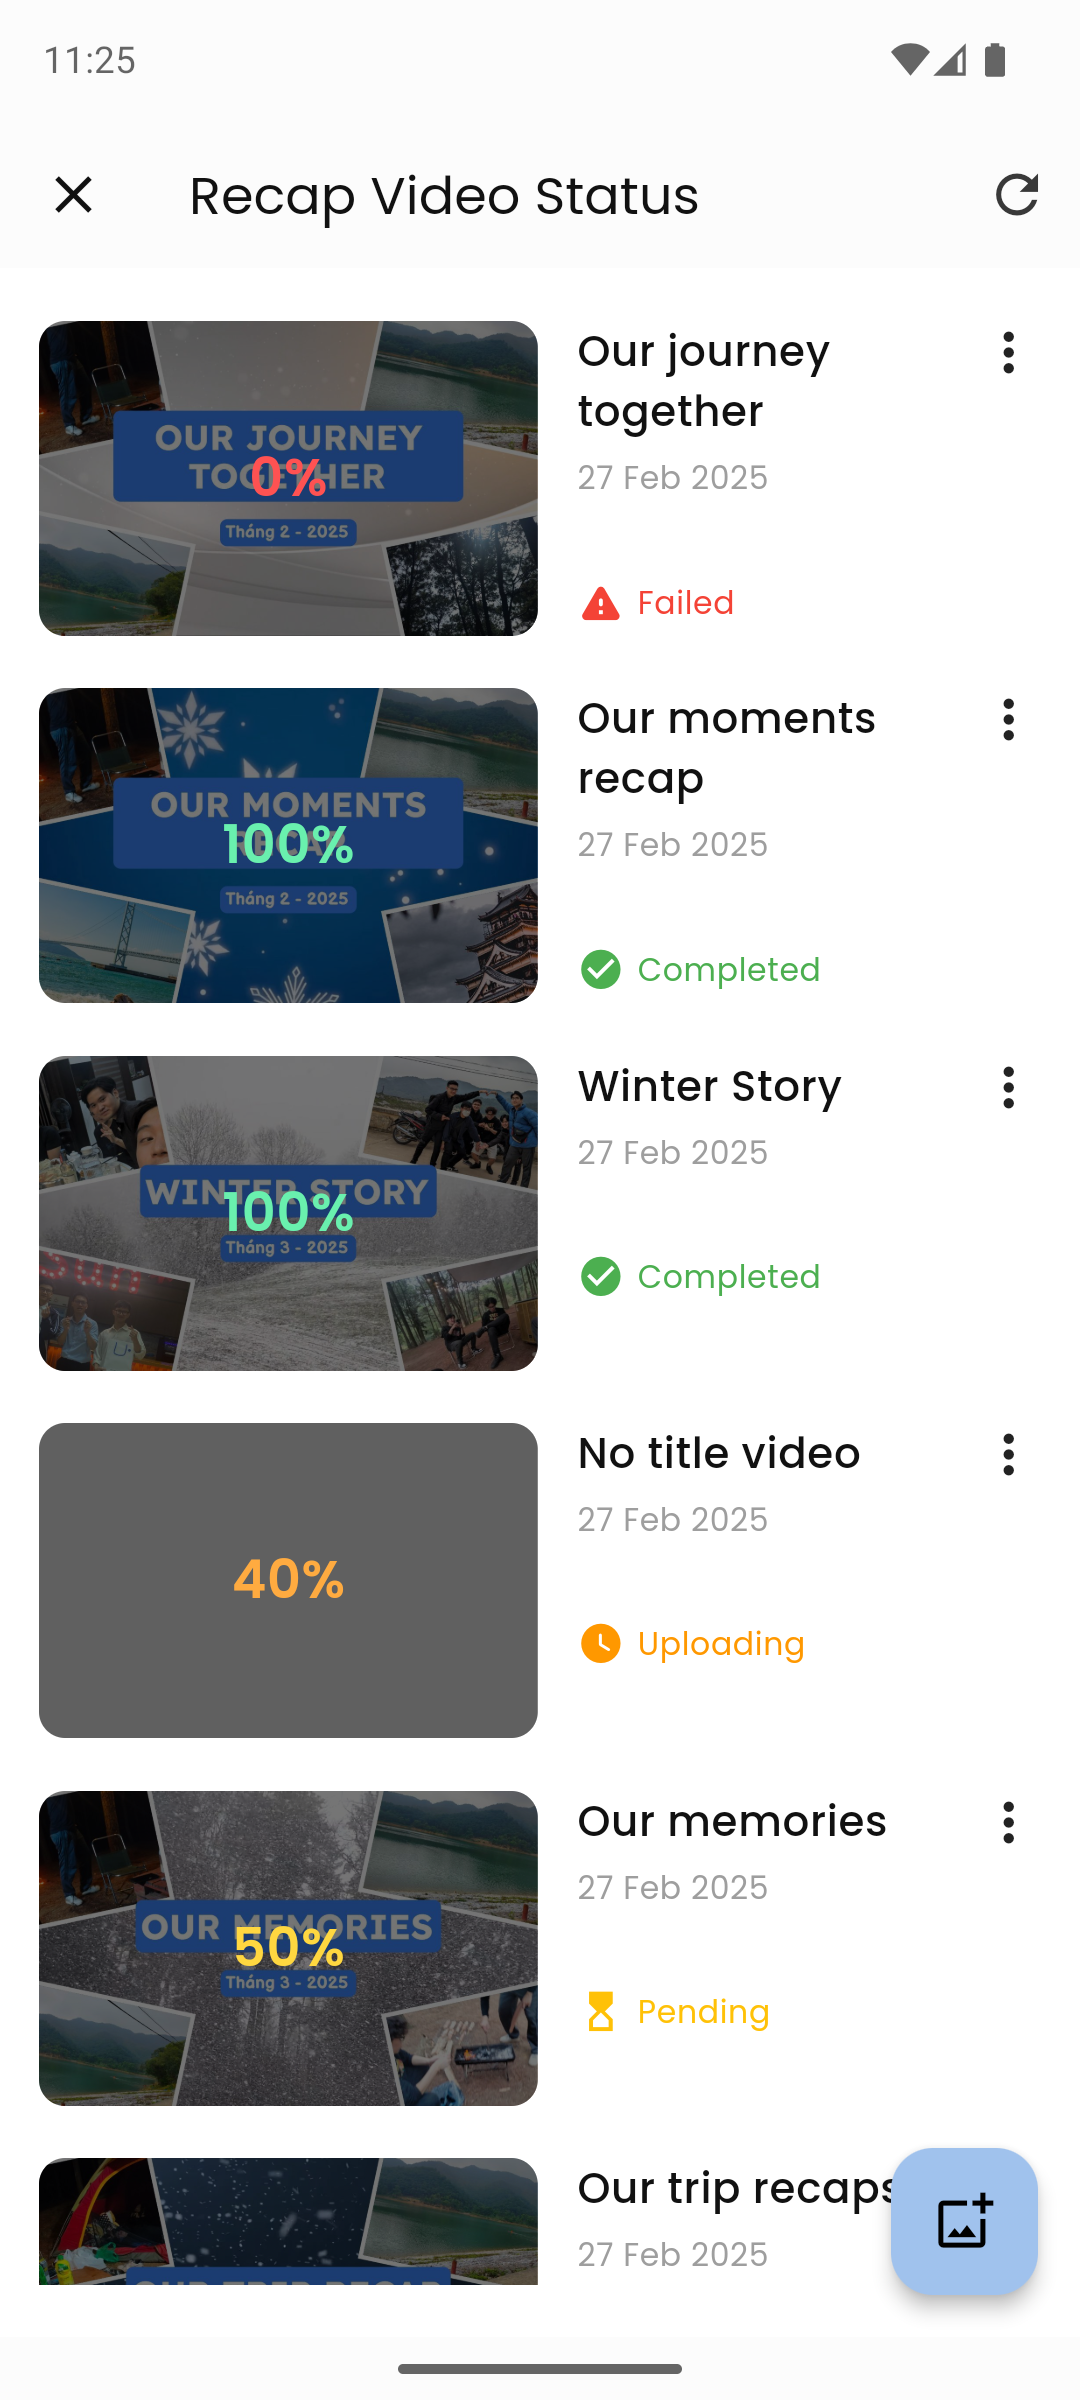
\includegraphics[width=1\linewidth]{figures/c4/4-2/video_1.png} 
        \caption{Danh sách video}
    \end{subfigure}
    \hfill
    \begin{subfigure}{0.32\textwidth}
        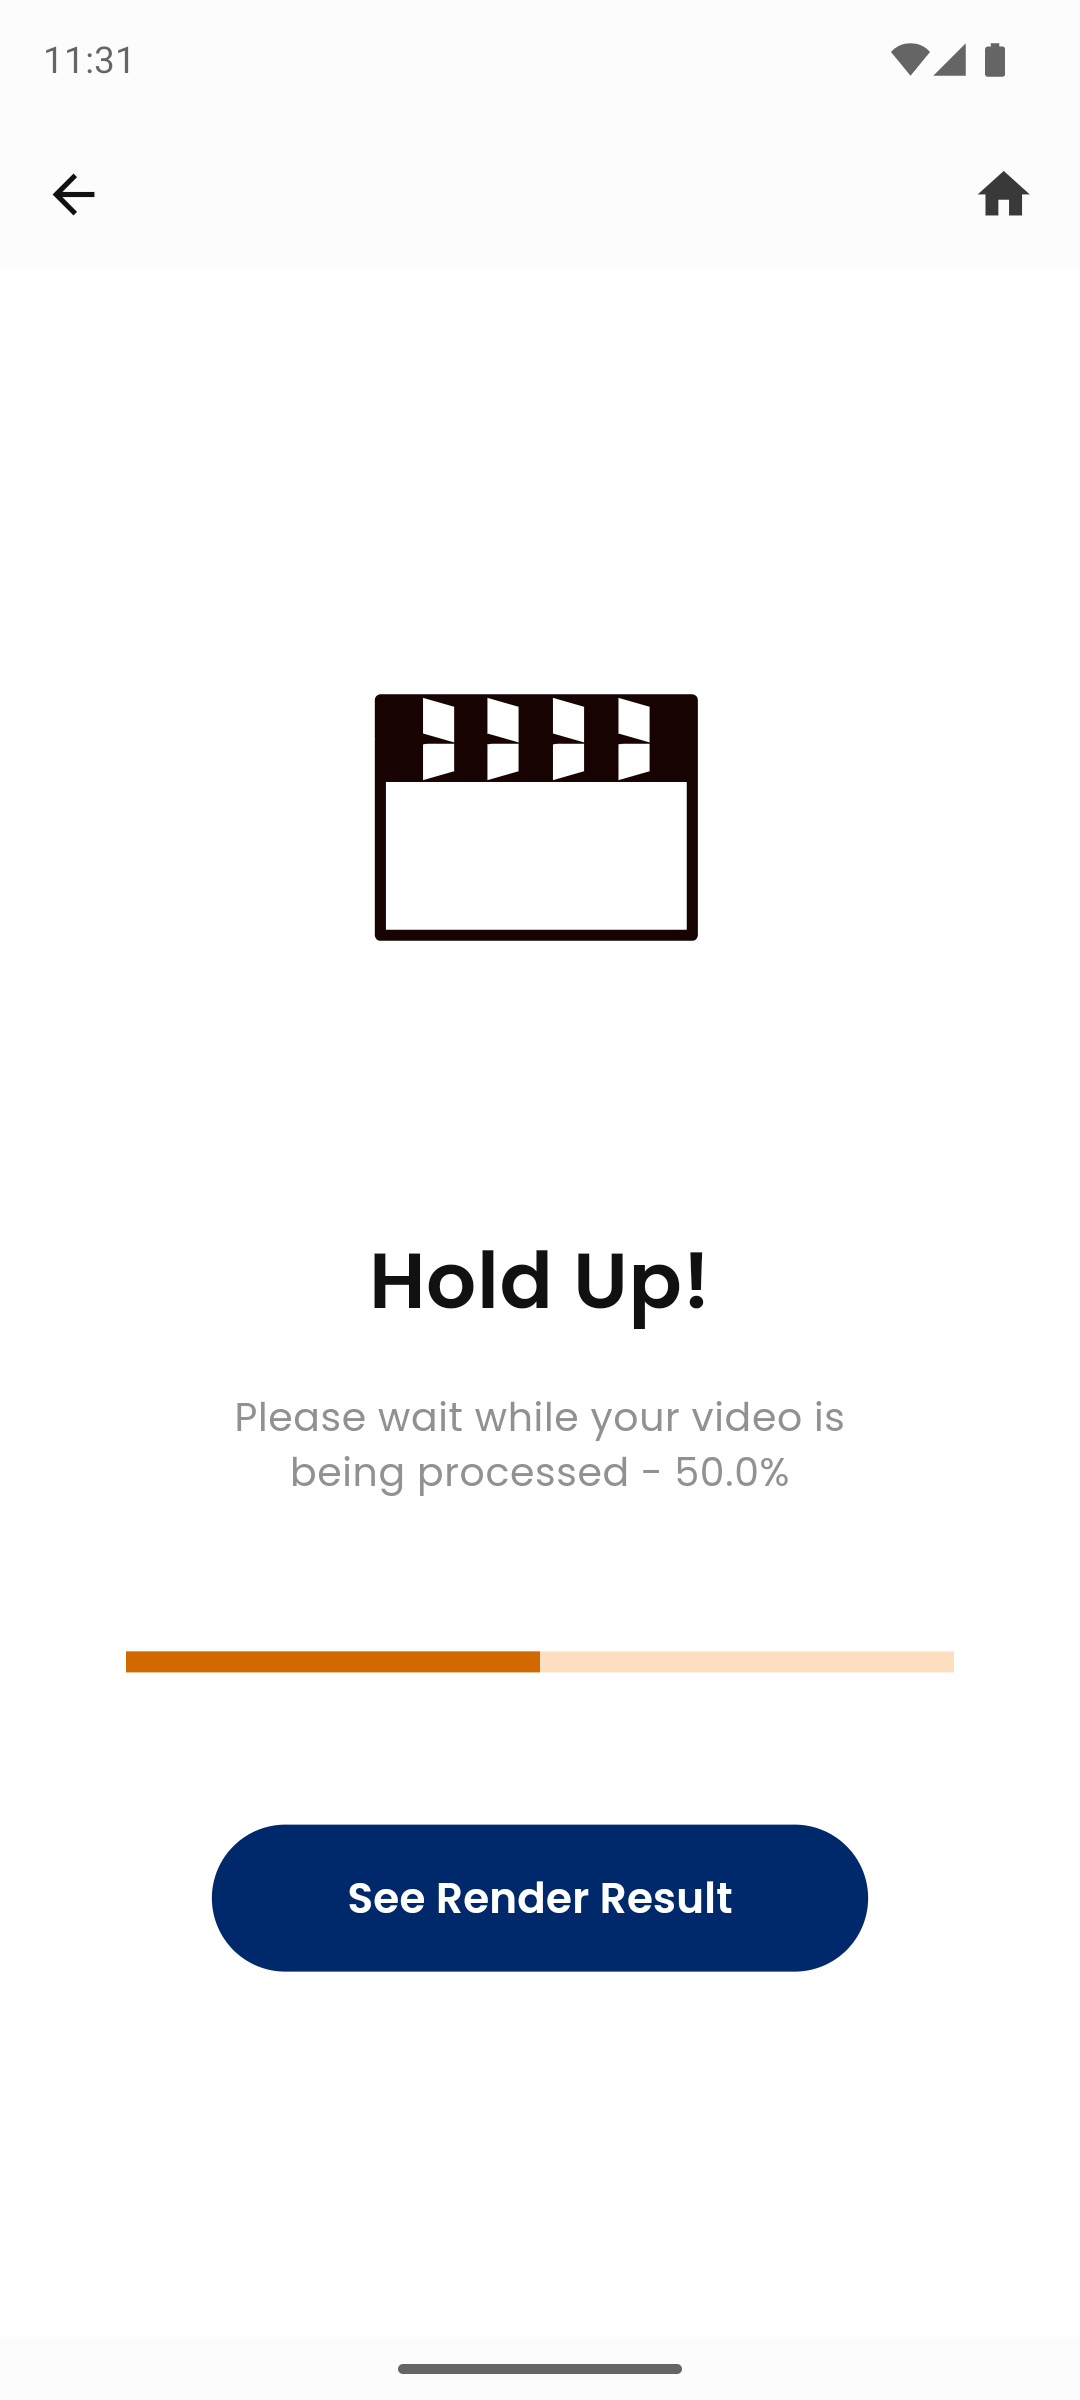
\includegraphics[width=1\linewidth]{figures/c4/4-2/video_2.png} 
        \caption{Xem trạng thái tạo video}
    \end{subfigure}
    \hfill
    \begin{subfigure}{0.32\textwidth}
        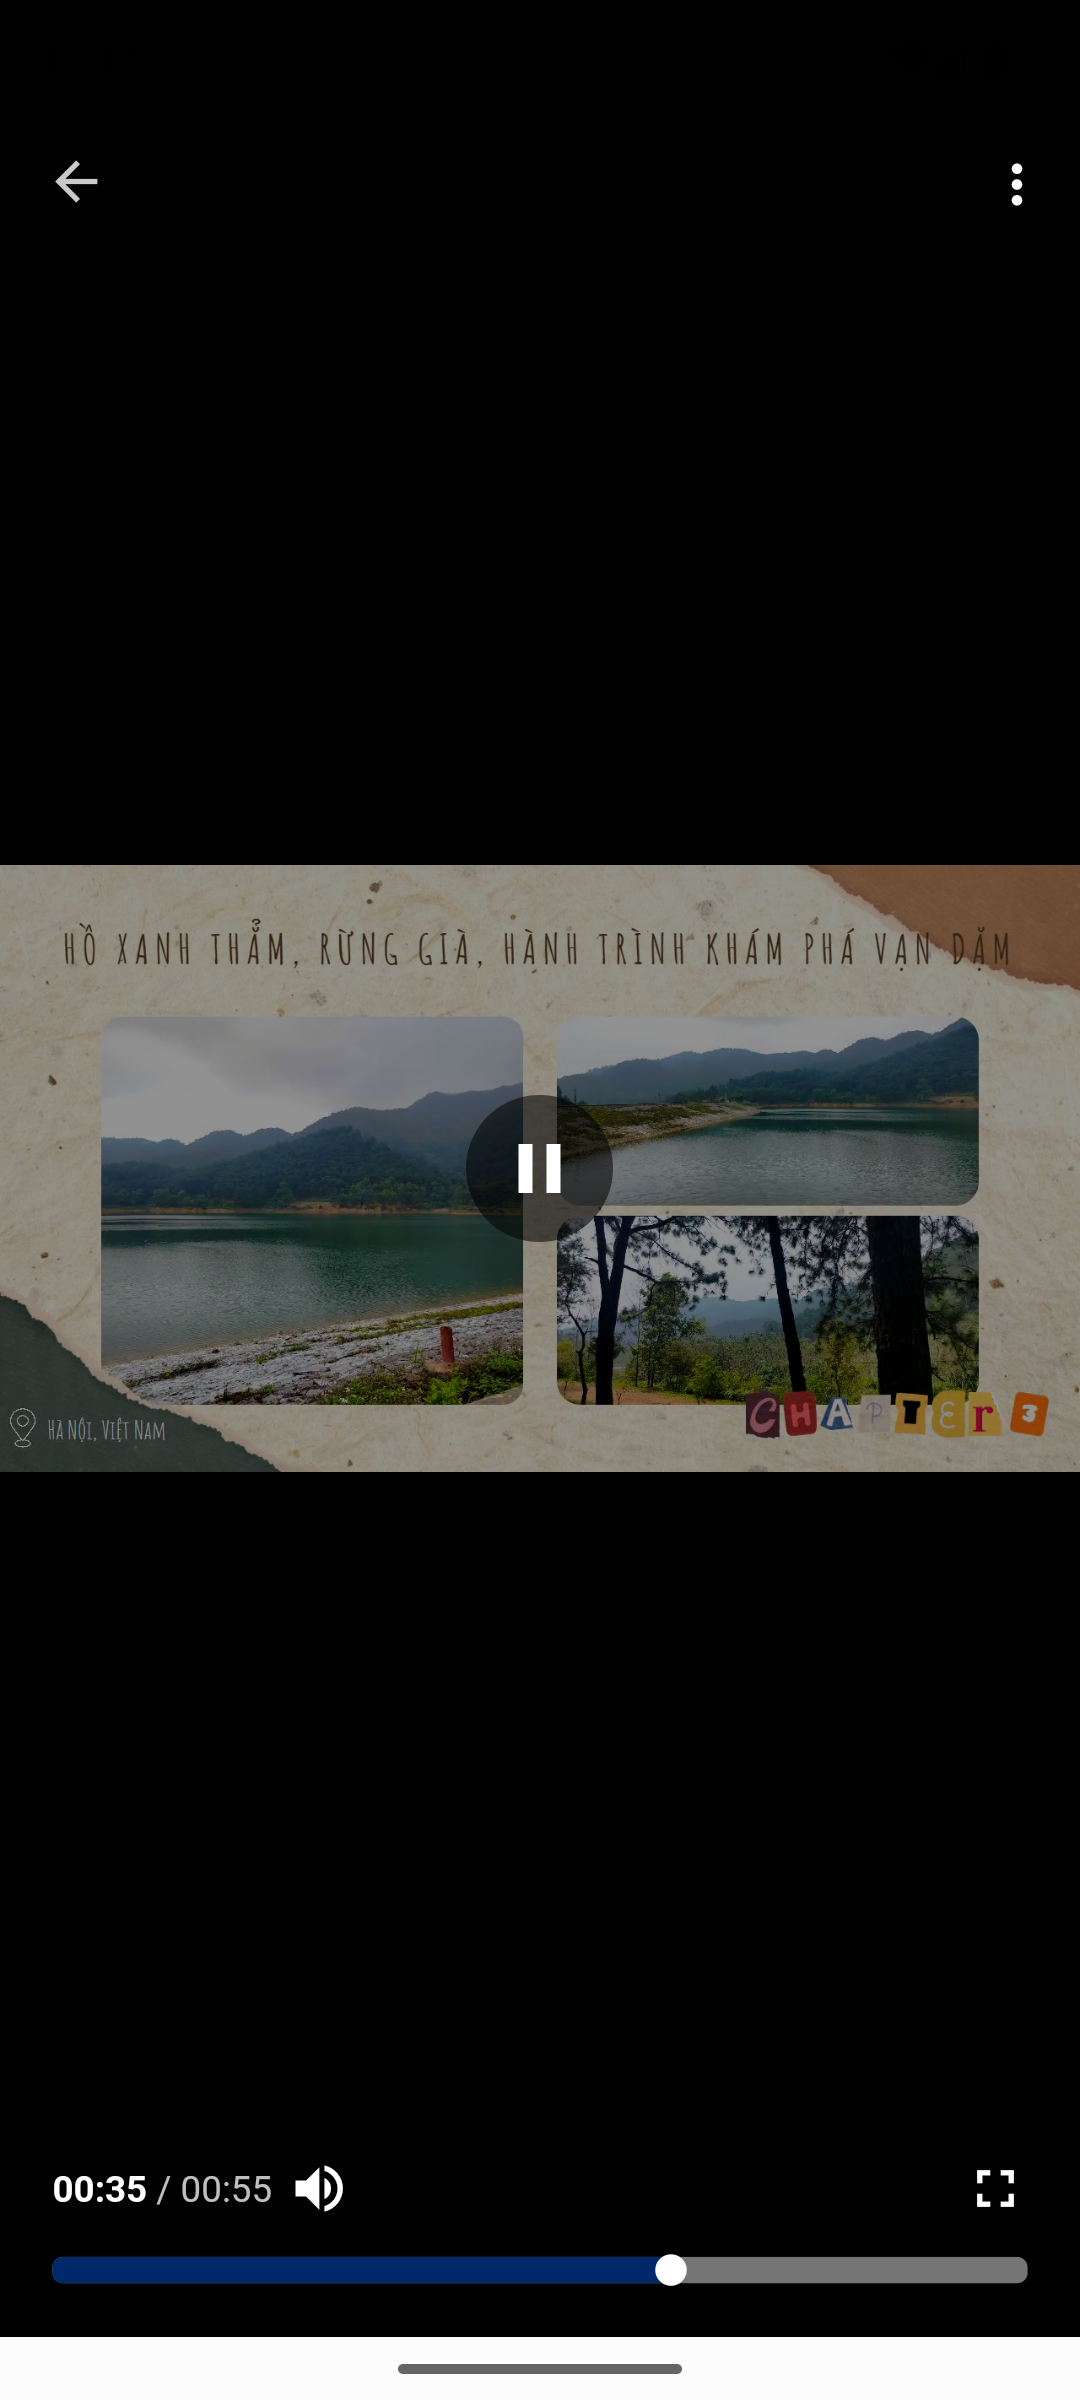
\includegraphics[width=1\linewidth]{figures/c4/4-2/video_3.png} 
        \caption{Xem video}
    \end{subfigure}
    \caption{Giao diện quản lý video recap.}
    \label{fig:video_recap}
\end{figure}

Ngoài ra, hệ thống cũng cung cấp tính năng tạo video cho người dùng và tùy chỉnh nhiều tùy chọn của video như chất lượng, chủ đề, nhạc nền, tiêu đề, v.v. như Hình \ref{fig:video_create}.

\begin{figure}[H]
    \centering
    \begin{subfigure}{0.48\textwidth}
        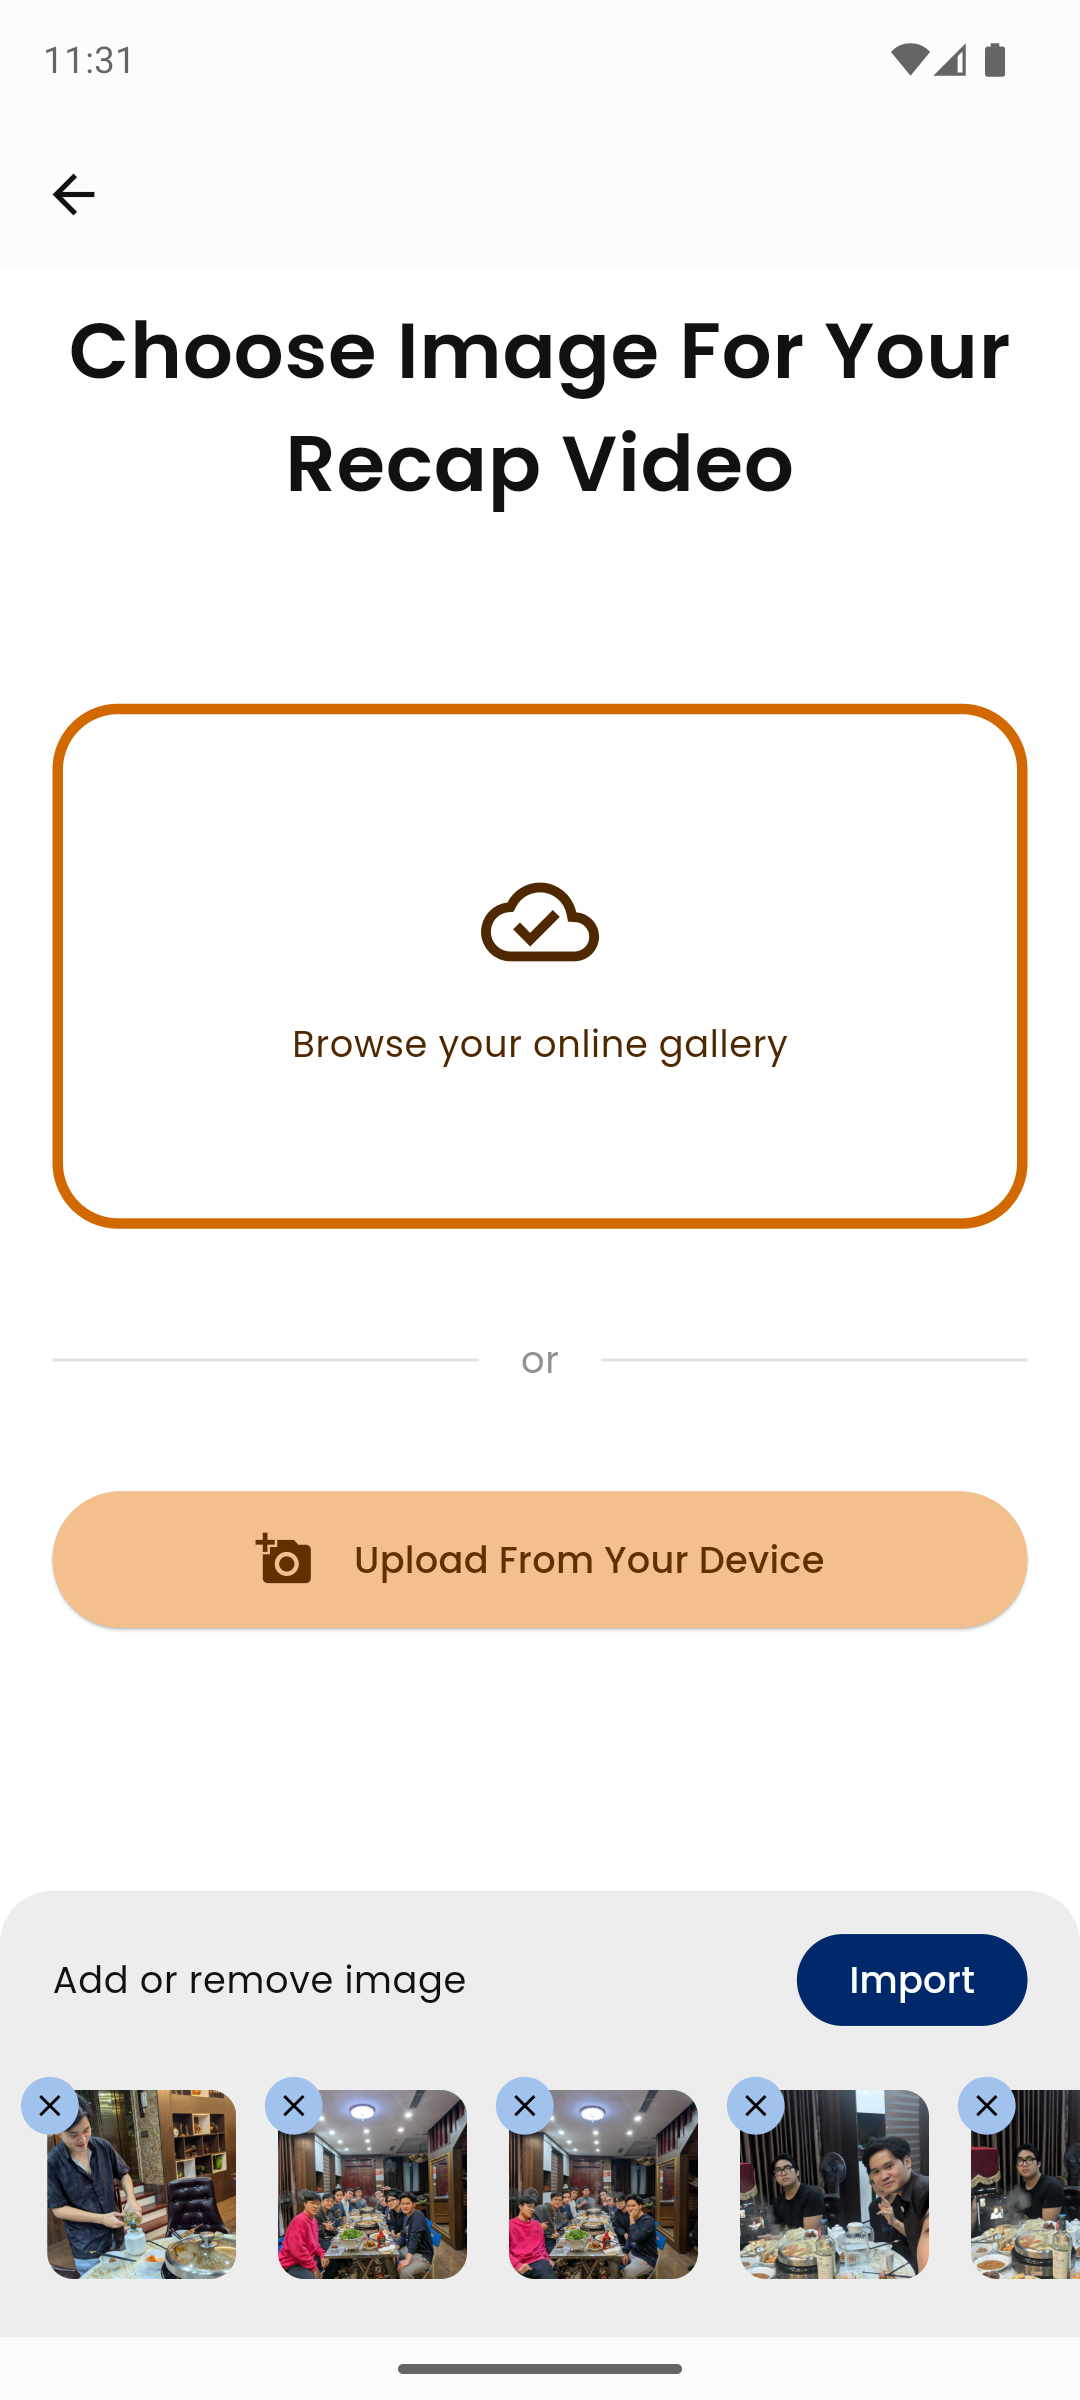
\includegraphics[width=1\linewidth]{figures/c4/4-2/create_video_1.png} 
        \caption{Tạo video}
    \end{subfigure}
    \hfill
    \begin{subfigure}{0.48\textwidth}
        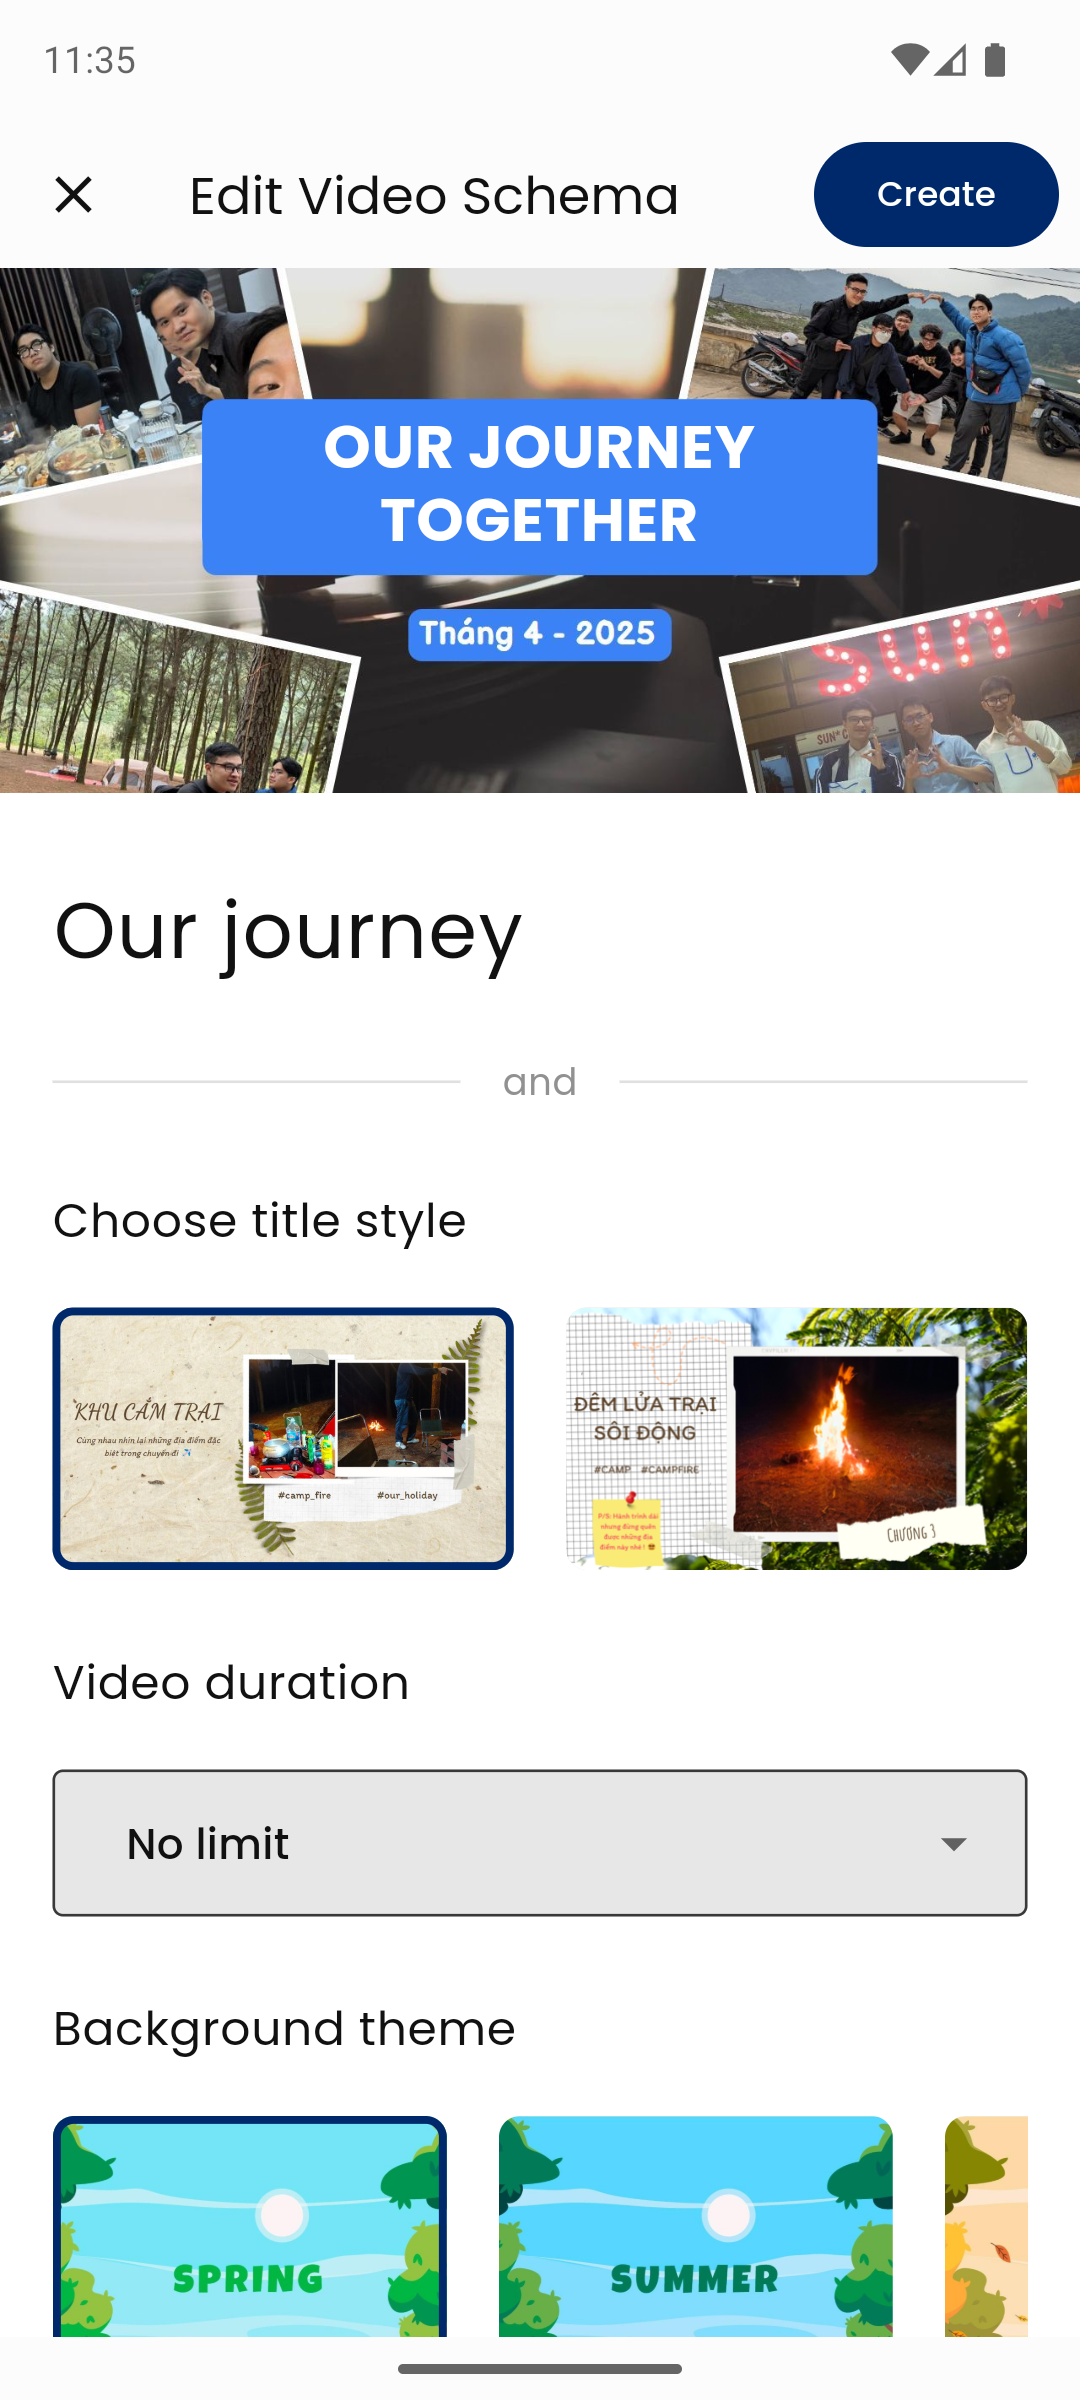
\includegraphics[width=1\linewidth]{figures/c4/4-2/create_video_2.png} 
        \caption{Chỉnh sửa tùy chọn video}
    \end{subfigure}
    \caption{Giao diện tạo video.}
    \label{fig:video_create}
\end{figure}

\subsection{Tìm kiếm ảnh}

Người dùng có thể tìm kiếm các ảnh trong hệ thống với các từ khóa khác nhau như tên album, tên ảnh, tên người dùng, hoặc các từ khóa khác liên quan đến ảnh. Giao diện tìm kiếm ảnh được thể hiện trong hình \ref{fig:search-screen}. 

\begin{figure}[H]
    \centering
    \begin{subfigure}{0.48\textwidth}
        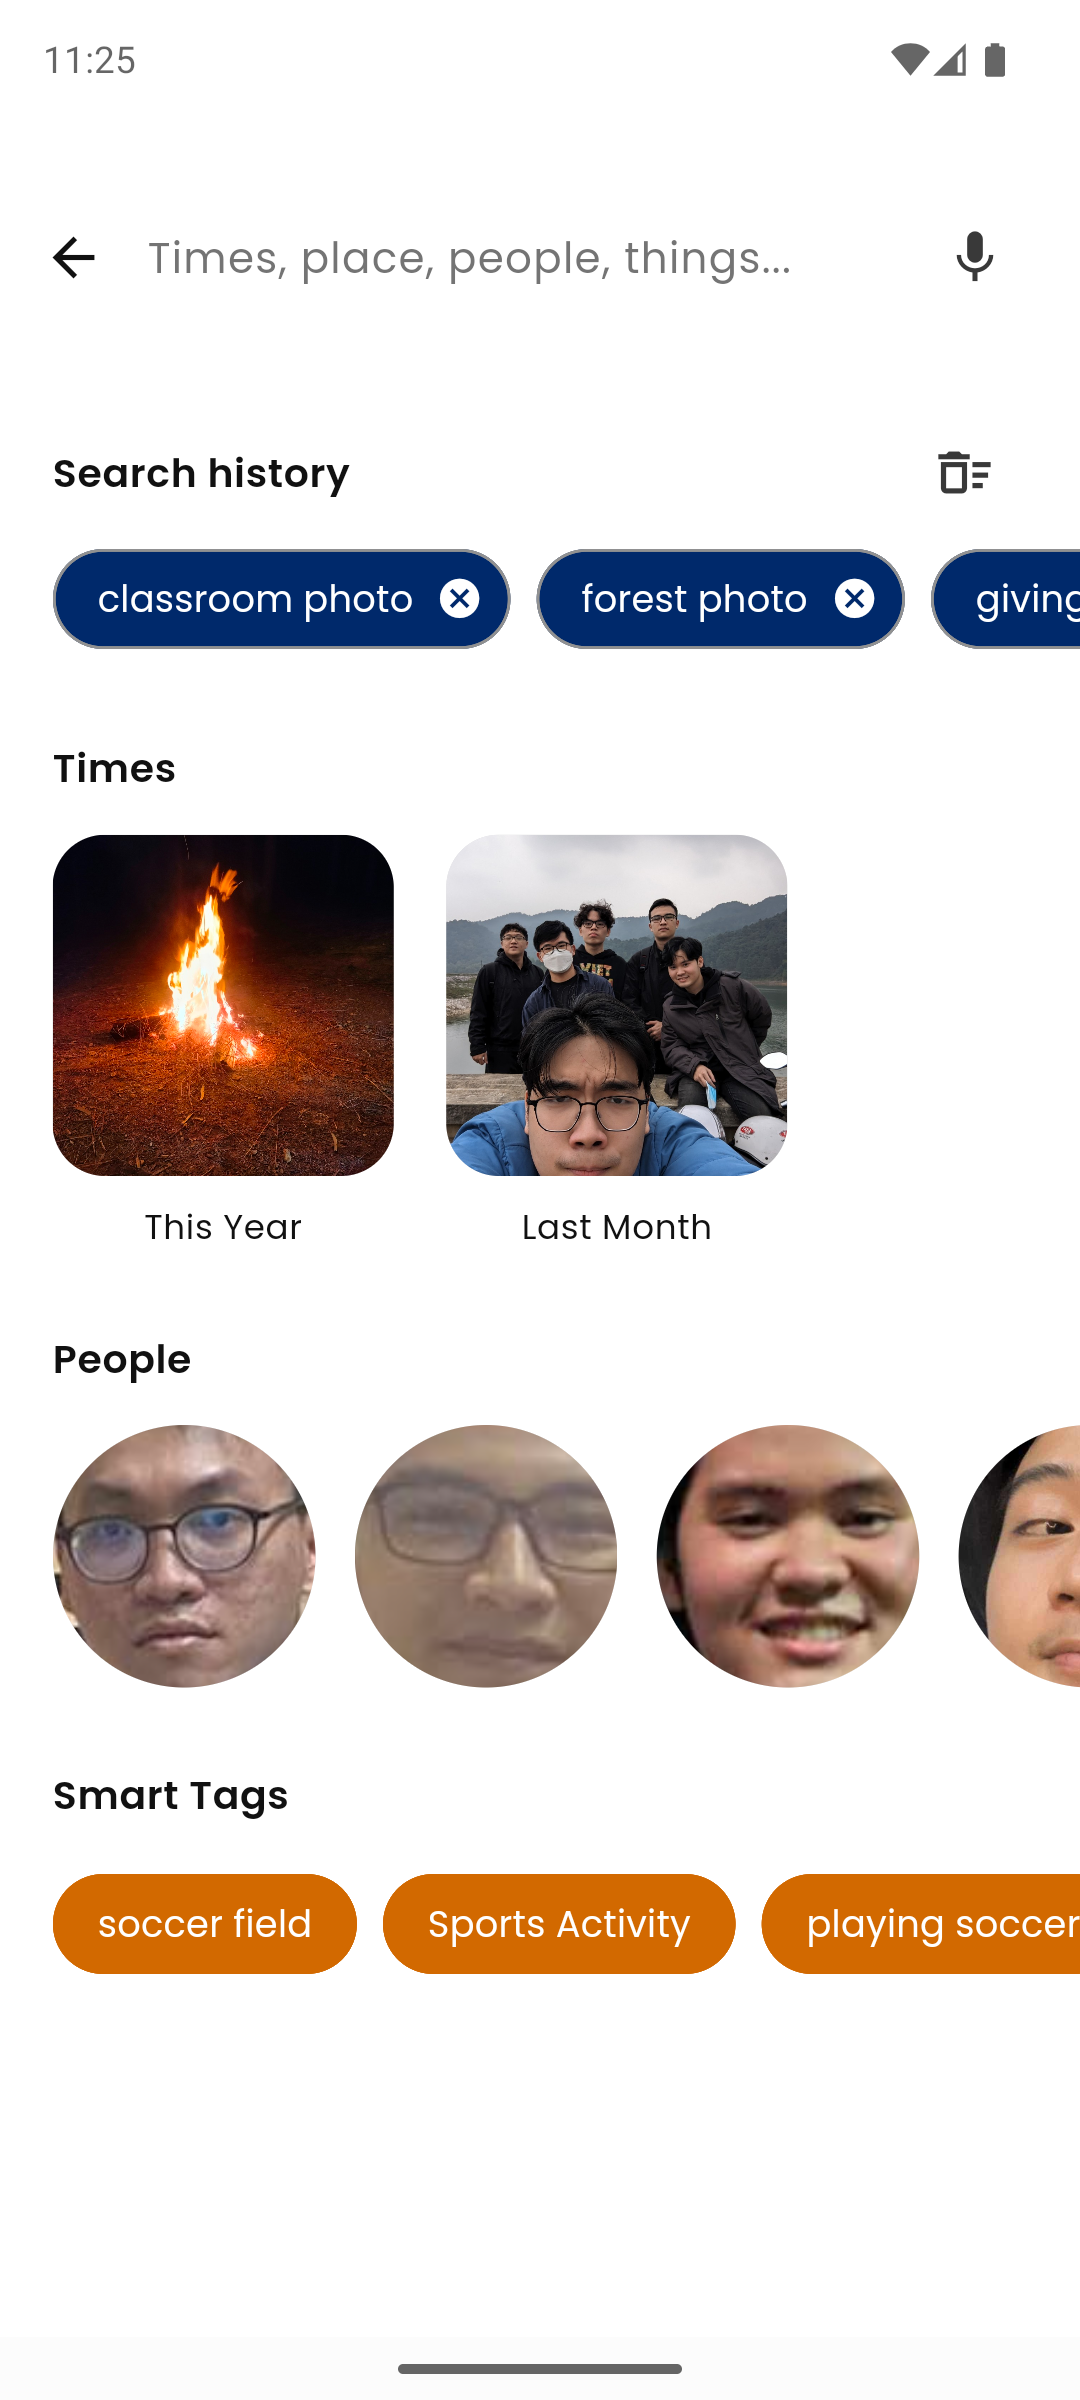
\includegraphics[width=1\linewidth]{figures/c4/4-2/search_1.png} 
        \caption{Các gợi ý tìm kiếm}
    \end{subfigure}
    \hfill
    \begin{subfigure}{0.48\textwidth}
        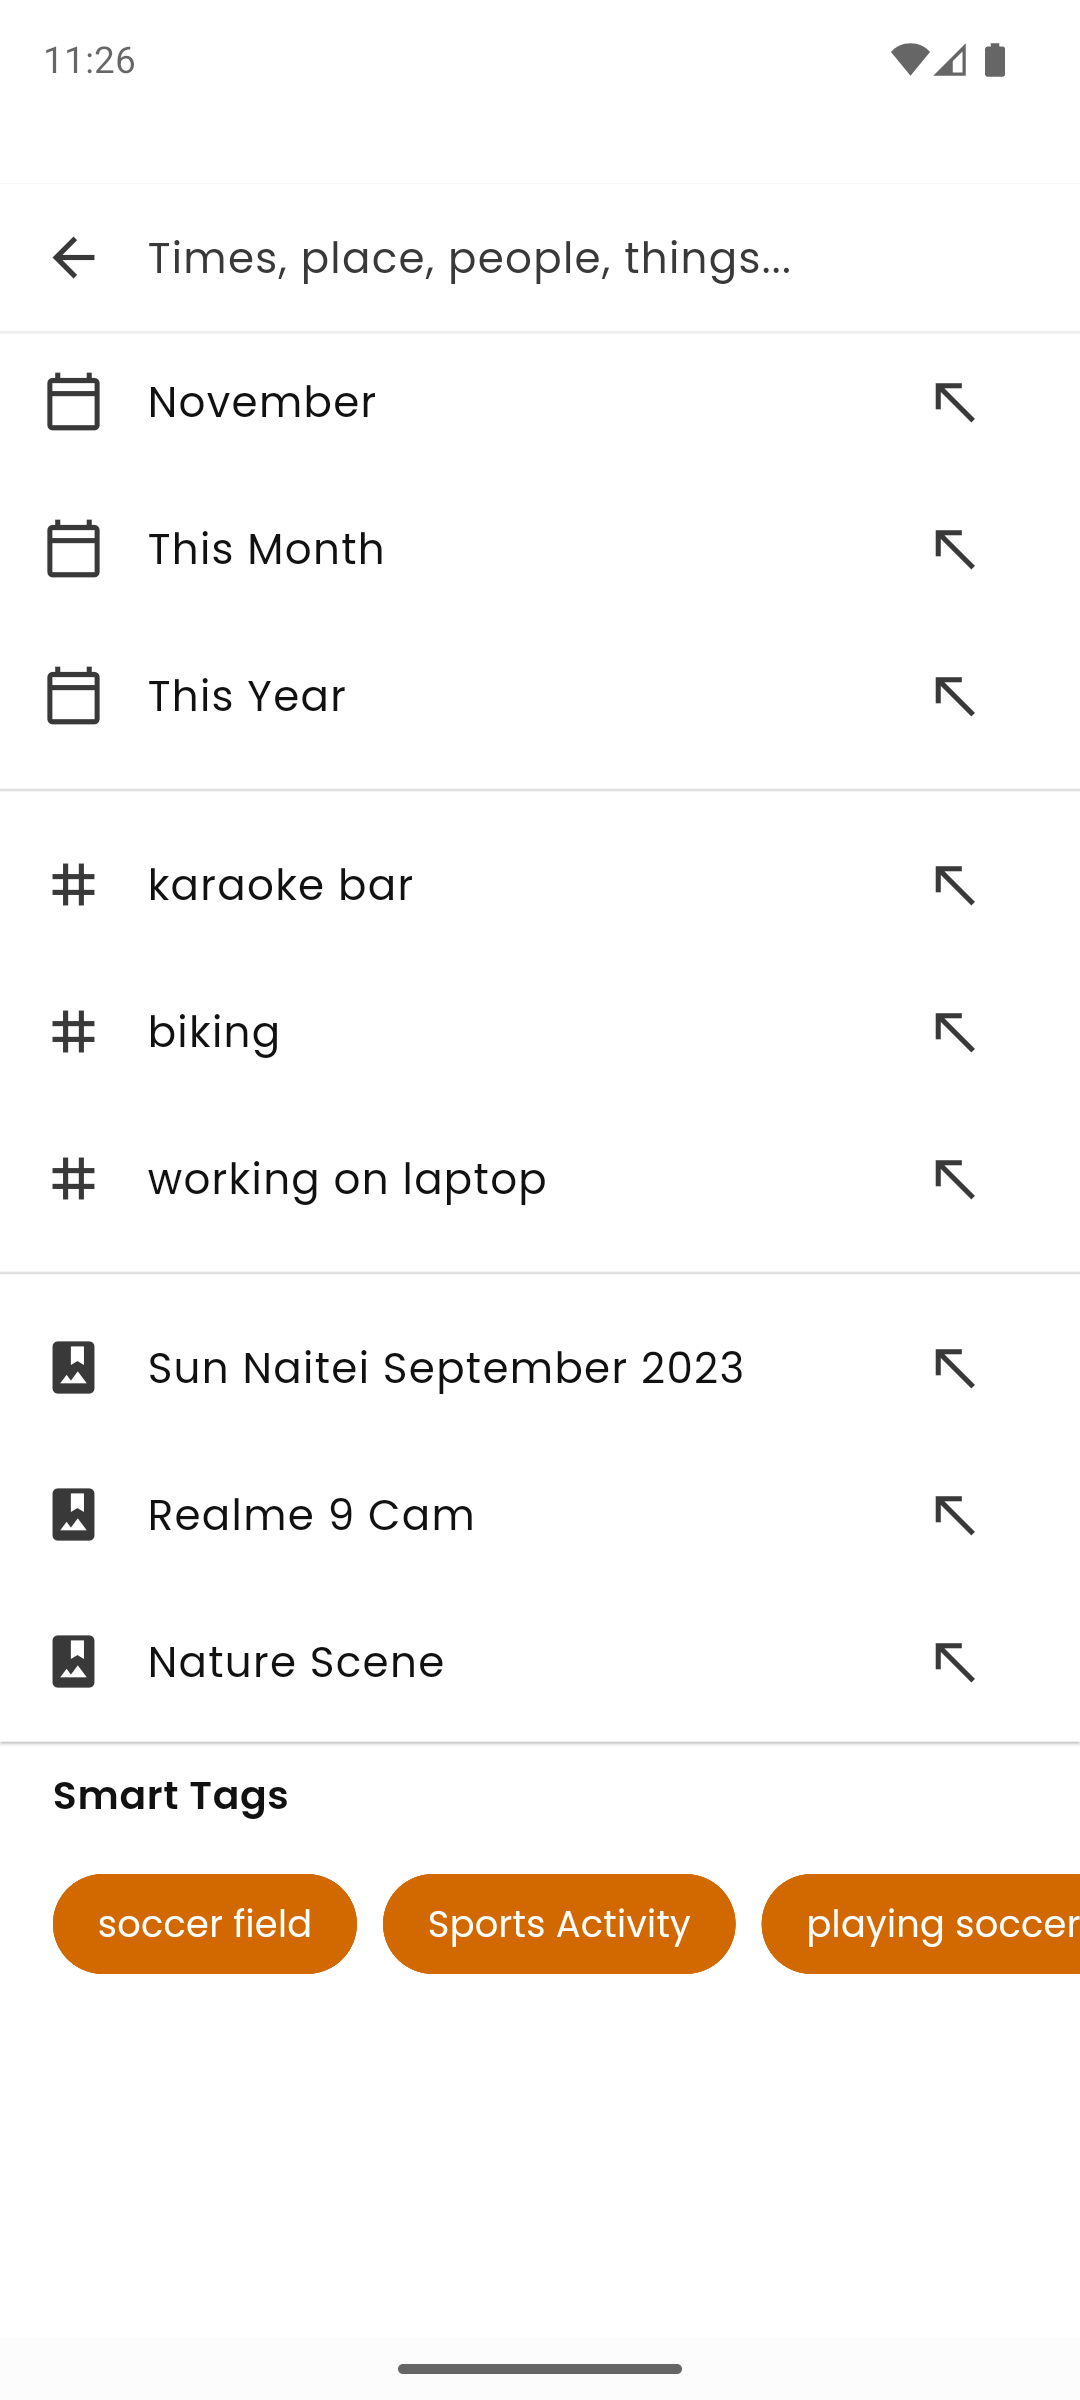
\includegraphics[width=1\linewidth]{figures/c4/4-2/search_2.png} 
        \caption{Gợi ý từ khóa tìm kiếm}
    \end{subfigure}
    \caption{Giao diện tìm kiếm.}
    \label{fig:search-screen}
\end{figure}

Kết quả tìm kiếm sẽ được hiện thành danh sách và được sắp xếp theo thời gian tải lên. Ngoài ra hệ thống cũng cung cấp tính năng tìm kiếm ảnh bằng giọng nói. Giao diện kết quả tìm kiếm và tìm kiếm bằng giọng nói được thể hiện trong Hình \ref{fig:search-result}.

\begin{figure}[H]
    \centering
    \begin{subfigure}{0.48\textwidth}
        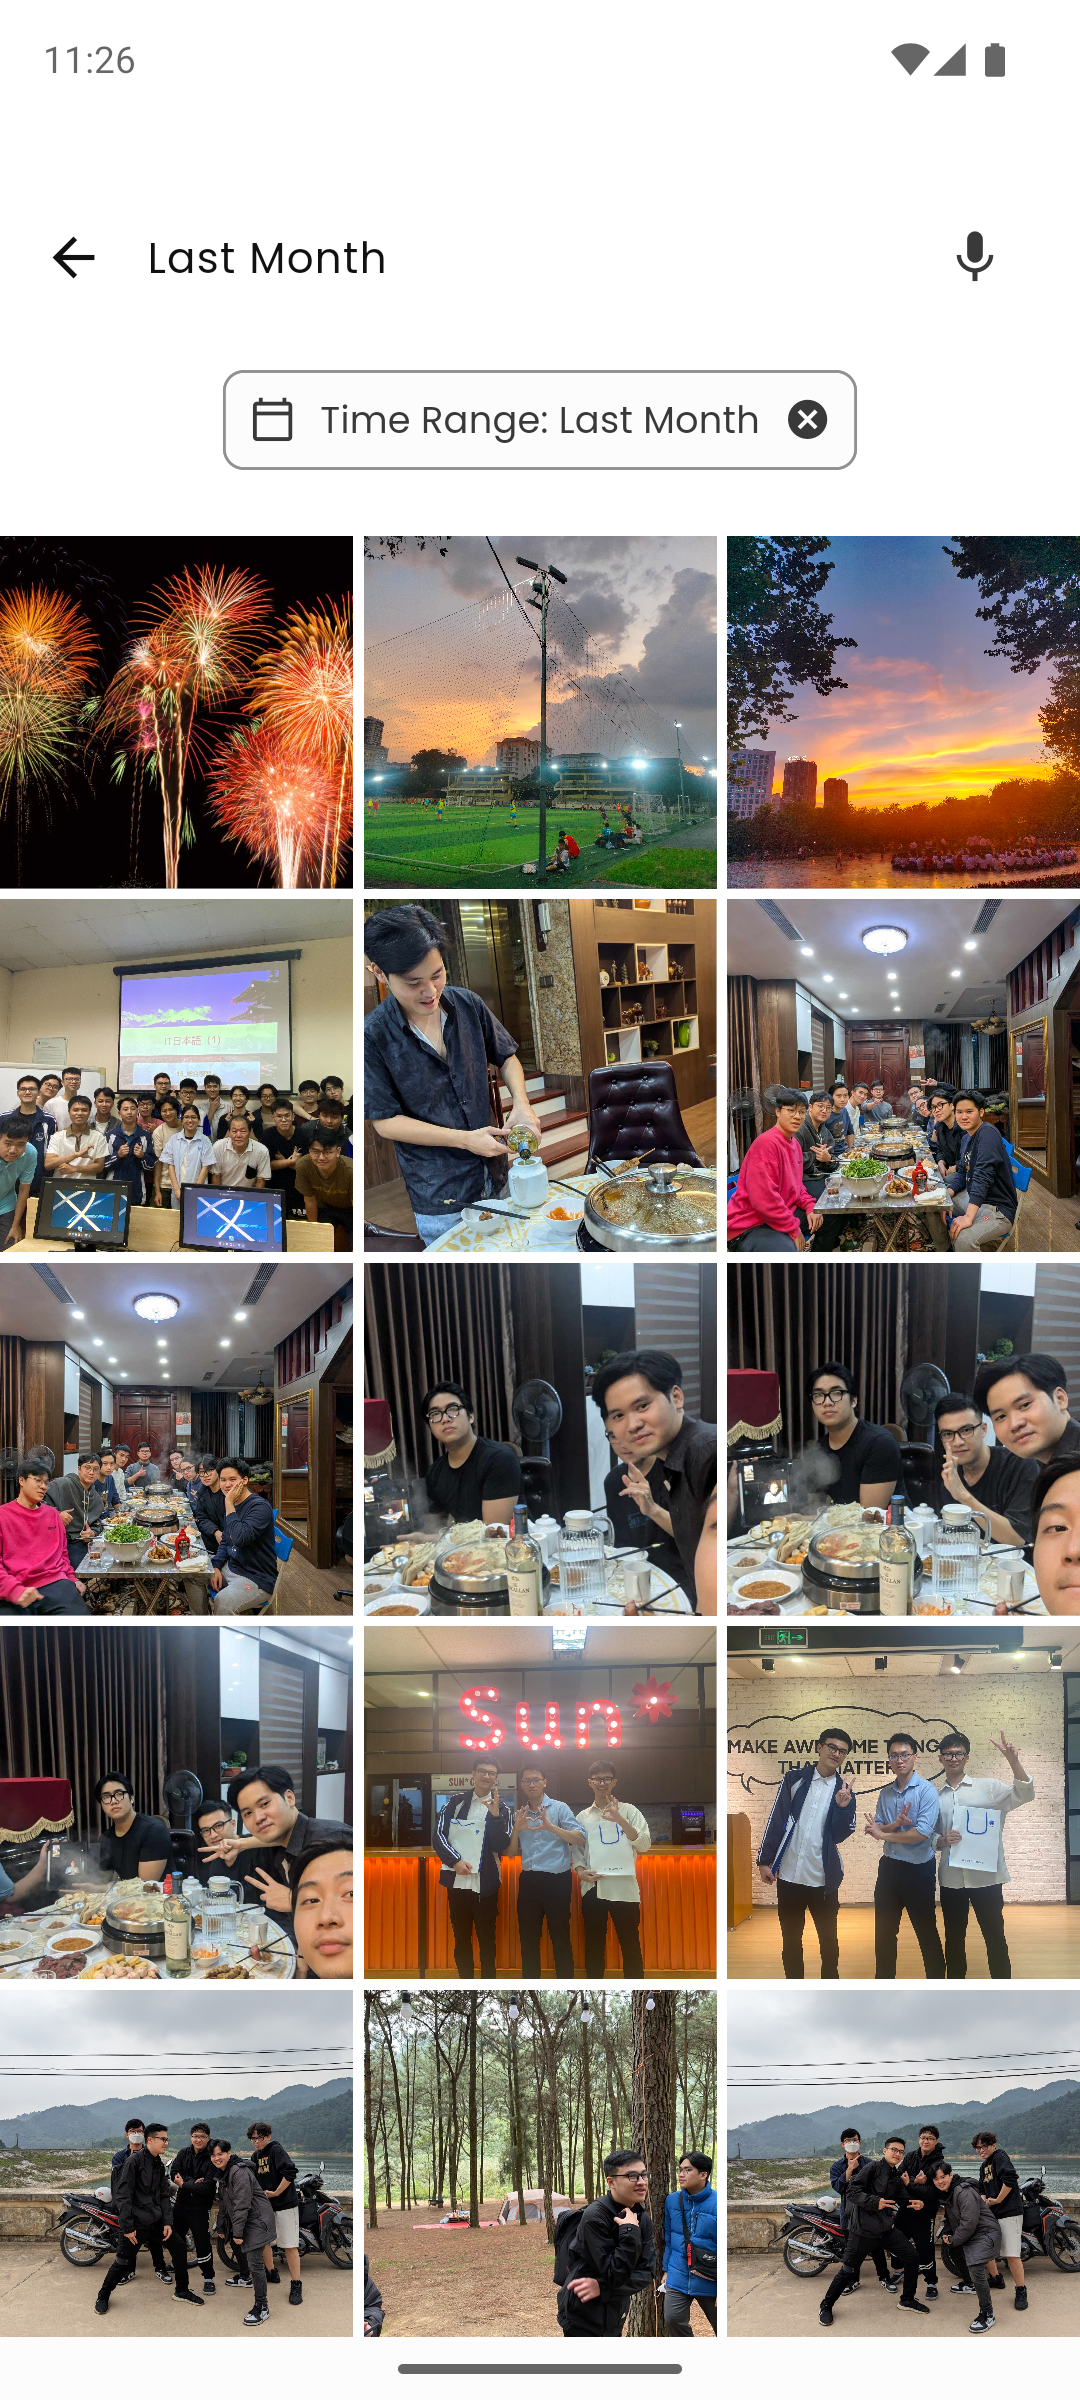
\includegraphics[width=1\linewidth]{figures/c4/4-2/search_4.png} 
        \caption{Kết quả tìm kiếm}
    \end{subfigure}
    \hfill
    \begin{subfigure}{0.48\textwidth}
        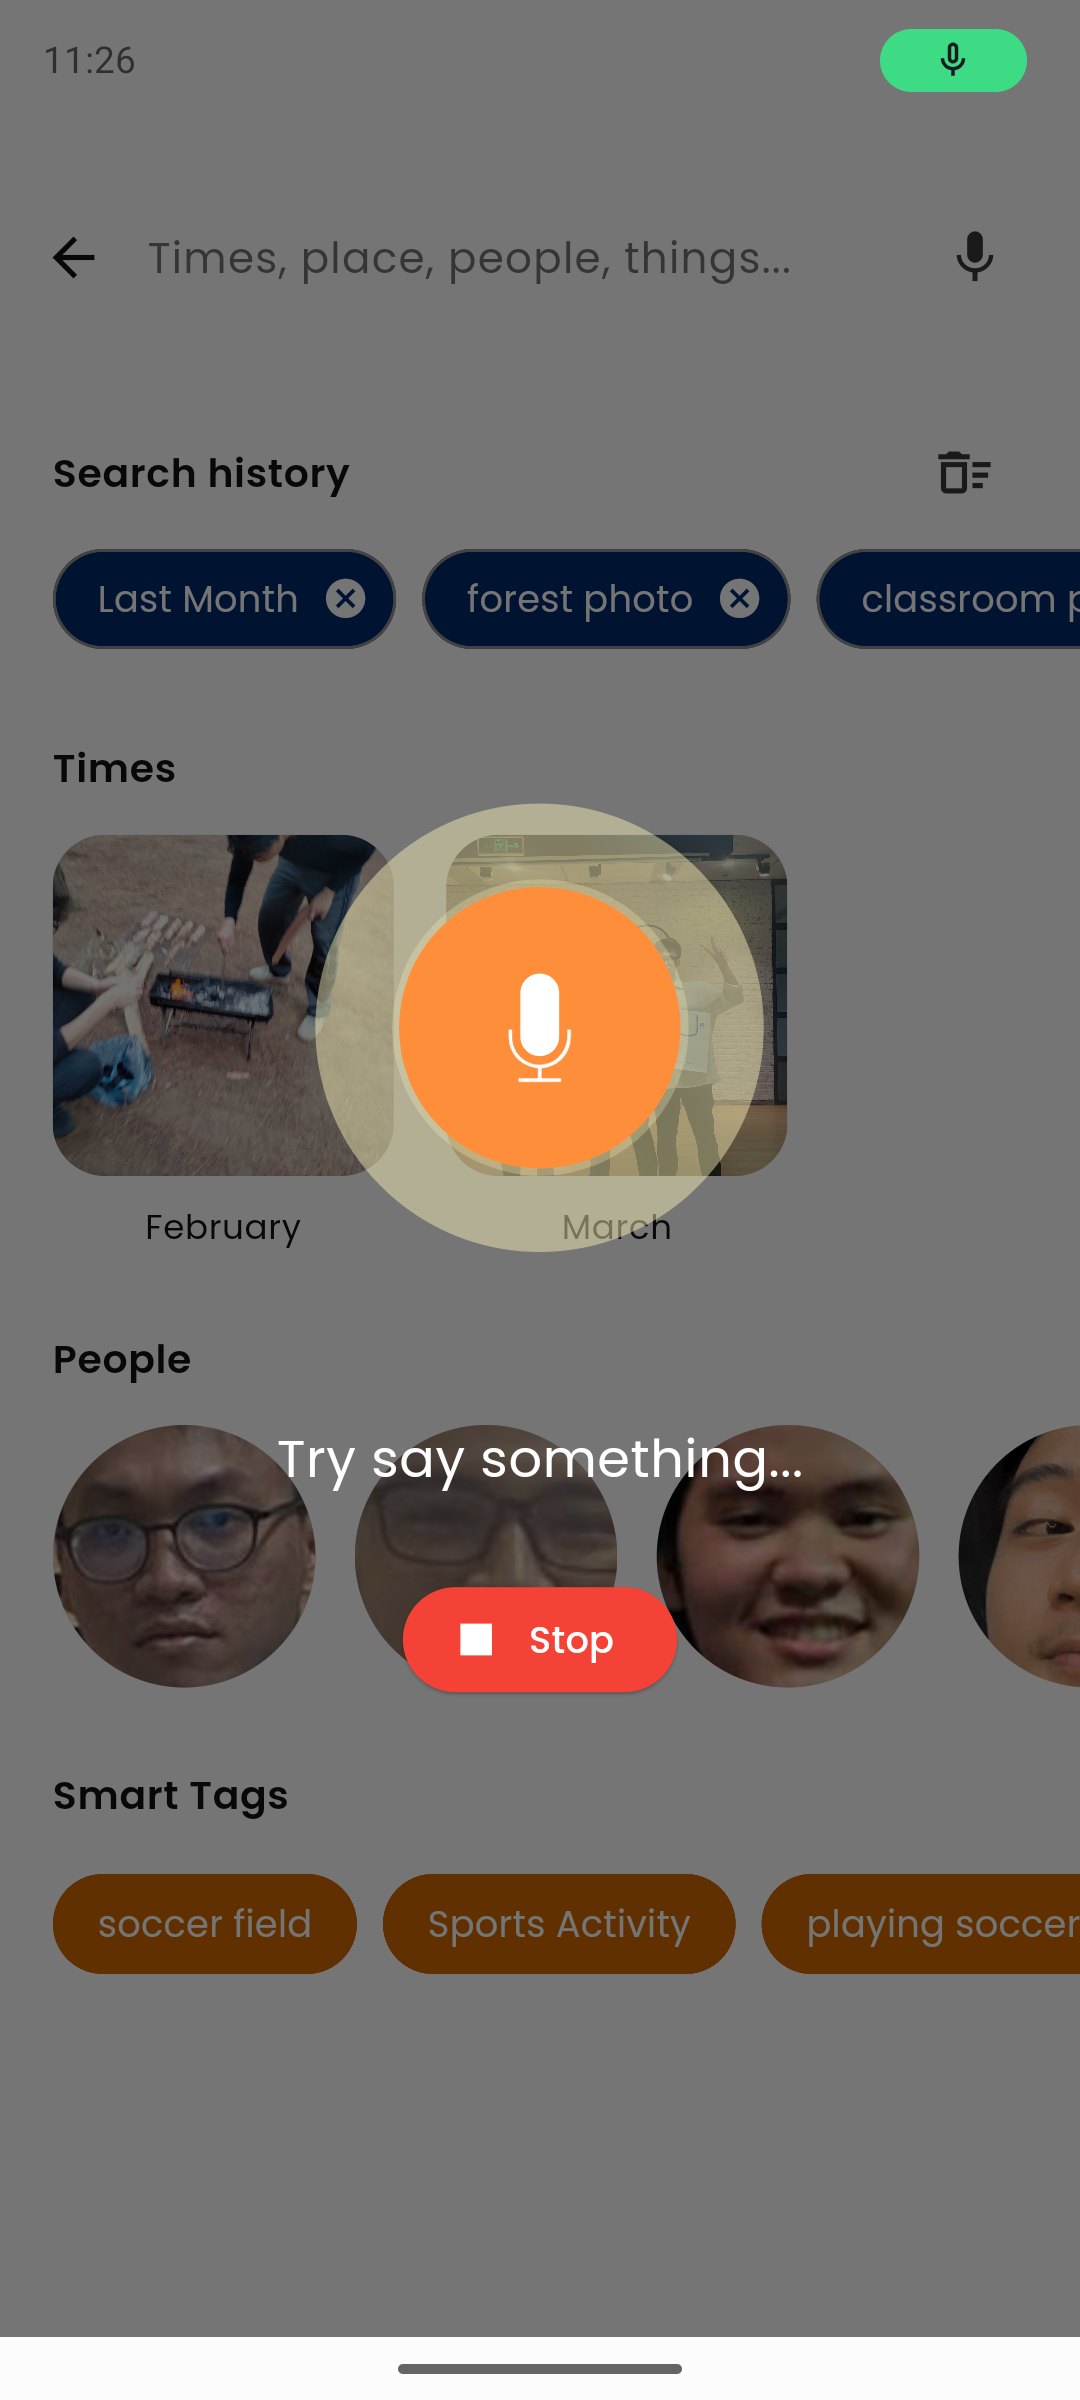
\includegraphics[width=1\linewidth]{figures/c4/4-2/search_3.png} 
        \caption{Tìm kiếm bằng giọng nói}
    \end{subfigure}
    \caption{Giao diện tìm kiếm (2).}
    \label{fig:search-result}
\end{figure}

\section{Kiểm thử cho hệ thống}

Chương này sẽ trình bày về các phương pháp kiểm thử hệ thống. Bao gồm các phương pháp kiểm thử logic như kiểm thử đơn vị và kiểm thử API. Ngoài ra, chương cũng sẽ trình bày về kết quả của các ca kiểm thử tương tác người dùng trên giao diện ứng dụng.

\subsection{Kiểm thử các xử lý logic}

Để đảm bảo hệ thống hoạt động ổn định và chính xác, các xử lý logic của hệ thống cần được kiểm thử kỹ lưỡng. Các kiểm thử này sẽ giúp phát hiện và sửa chữa các lỗi trong mã nguồn, đảm bảo rằng các chức năng của hệ thống hoạt động như mong đợi. Các kiểm thử này bao gồm kiểm thử đơn vị (Unit Testing) và kiểm thử API (API Testing).
\subsubsection{Kiểm thử đơn vị}


\textbf{Phạm vi kiểm thử}

Phạm vi kiểm thử đơn vị cho ứng dụng Smart Gallery bao gồm kiểm thử các hàm xử lý và các lớp xử lý logic của 2 server labeling ảnh và server tạo video. 

\textbf{Môi trường kiểm thử}

Môi trường kiểm thử cho các xử lý logic gồm có: 
\begin{itemize}
    \item JestJS\cite{jestJS}: là một công cụ được sử
    dụng để kiểm thử đơn vị được tích hợp sẵn trong NodeJs.
    \item pytest\cite{pytest}: là một thư viện kiểm thử đơn vị mạnh mẽ và linh hoạt cho Python. Kết hợp song song với unittest\cite{unittest}, pytest giúp kiểm thử các hàm xử lý logic của server labeling ảnh.
\end{itemize}

\textbf{Kết quả kiểm thử}

Độ phủ và kết quả kiểm thử xử lý logic như Hình \ref{fig:jest-testing} và Hình \ref{fig:pytest-testing}.

\begin{figure}[H]
    \centering  
    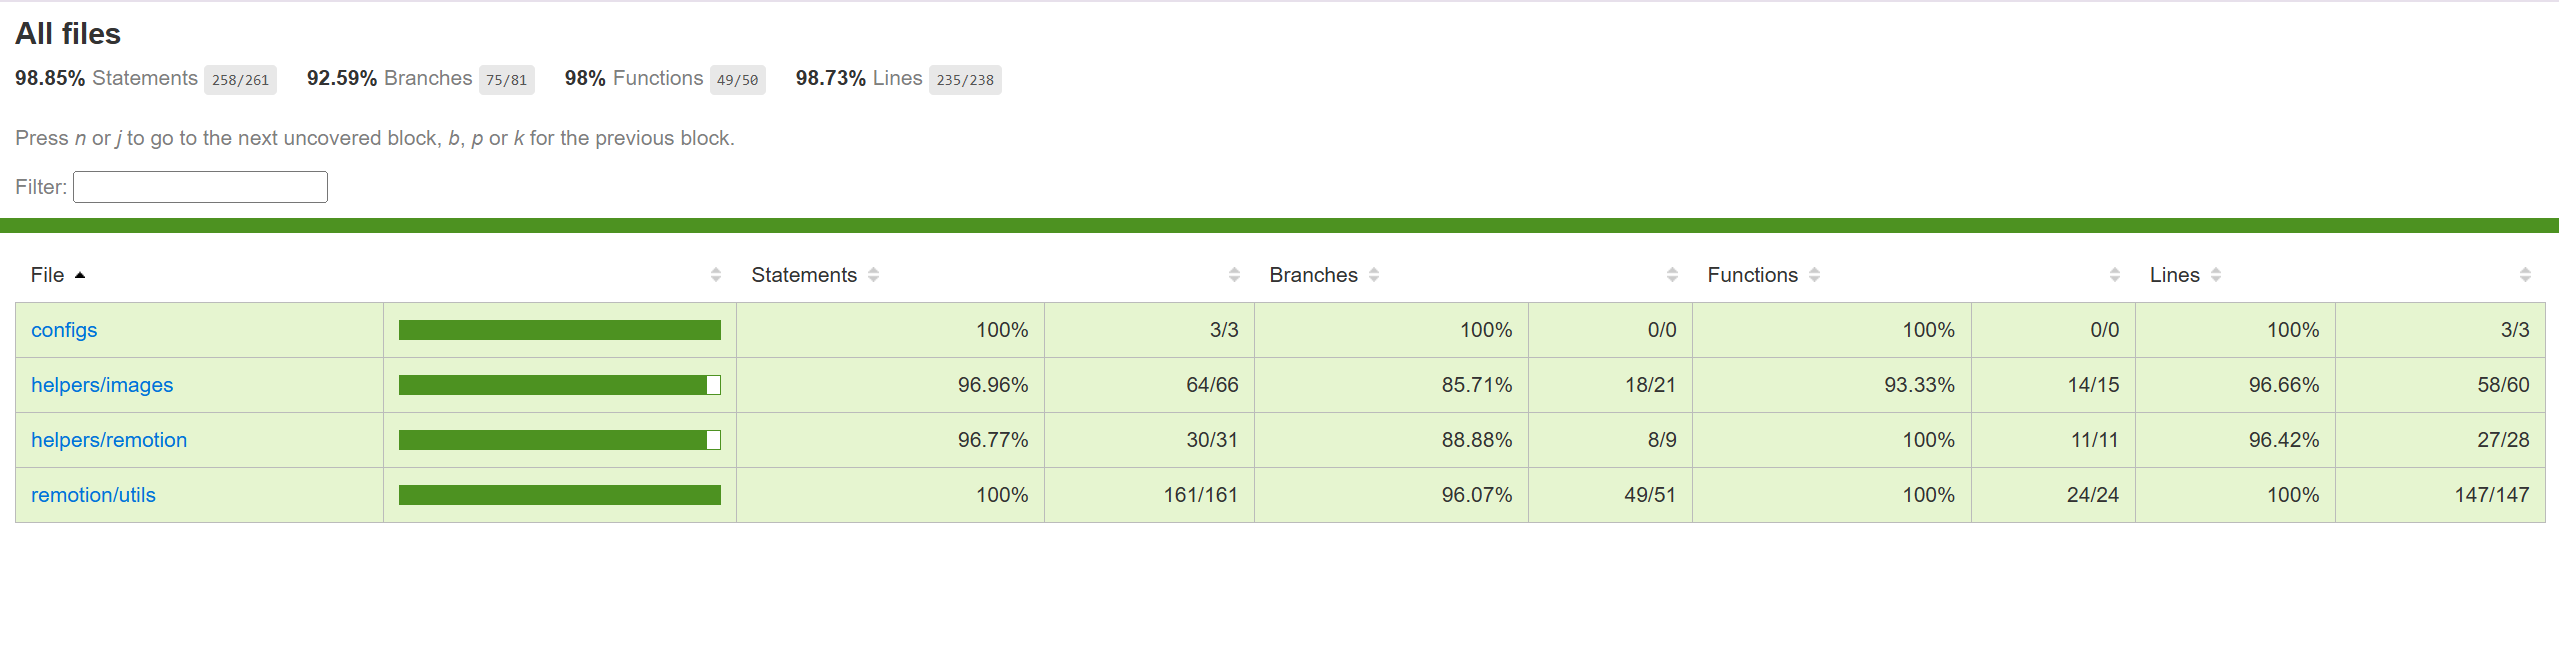
\includegraphics[width=1\textwidth]{figures/c4/4-3/jest.png}
    \caption{Độ phủ kiểm thử xử lý logic với JestJS.}
    \label{fig:jest-testing}
\end{figure}

% \begin{figure}[H]
%     \centering  
%     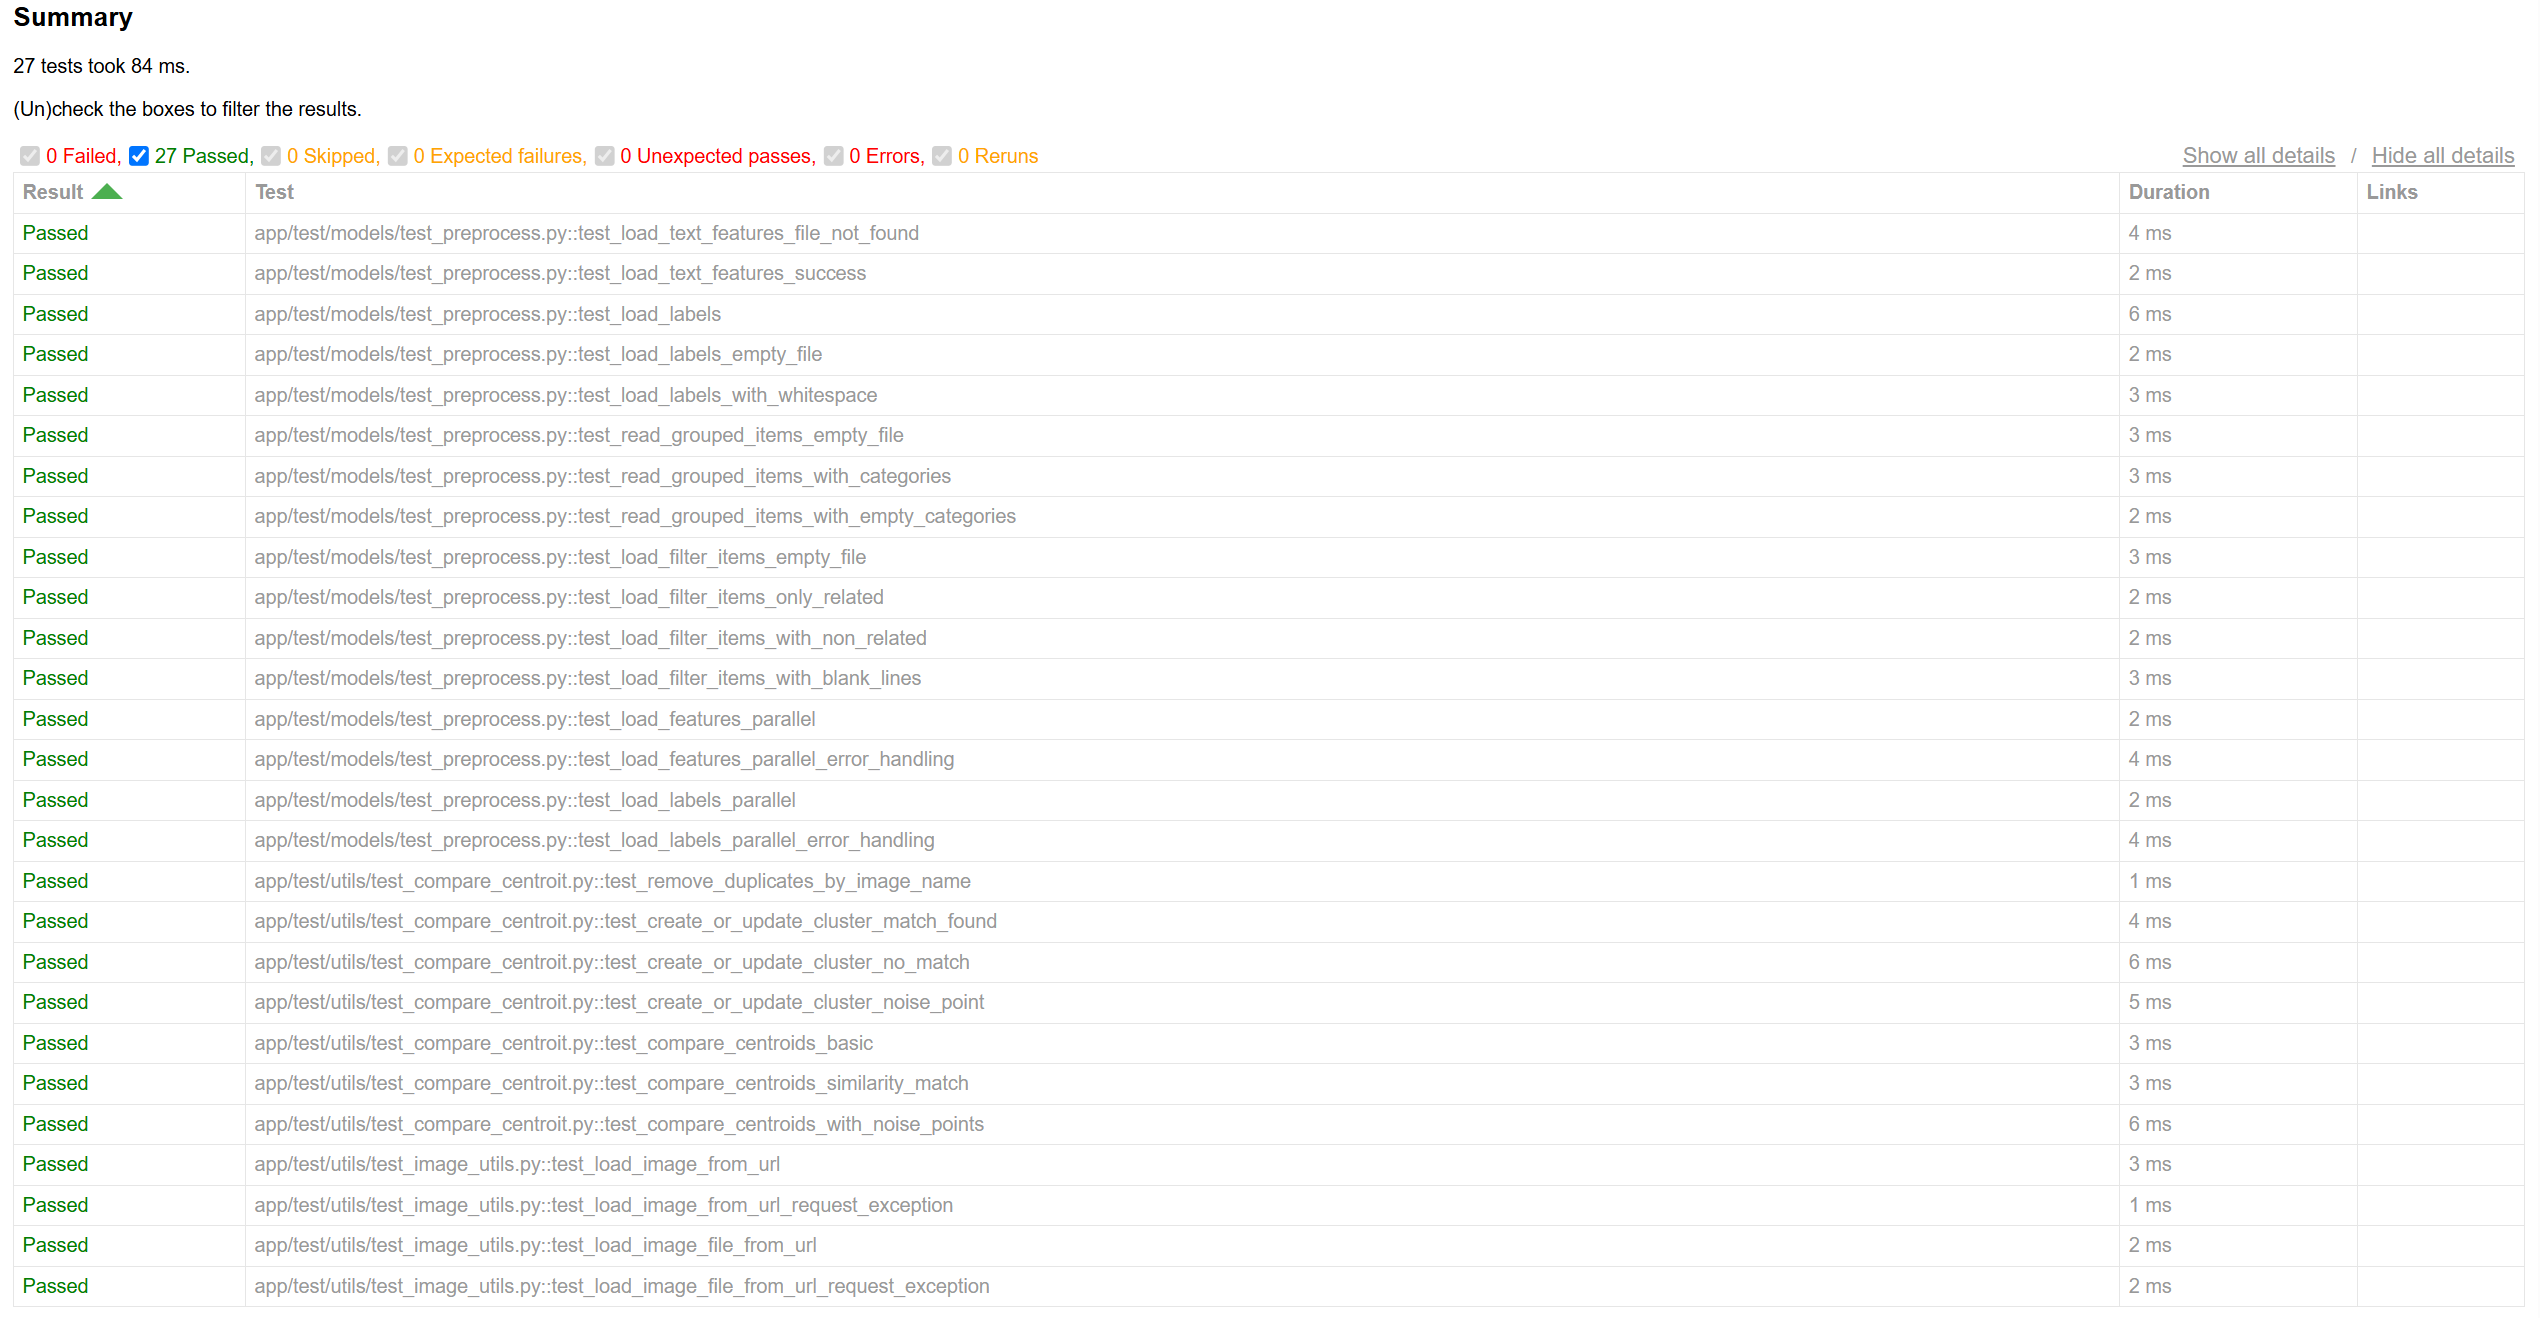
\includegraphics[width=1\textwidth]{figures/c4/4-3/pytest.png}
%     \caption{Kết quả các ca kiểm thử đơn vị với Pytest.}
%     \label{fig:pytest-coverage}
% \end{figure}

\begin{figure}[H]
    \centering  
    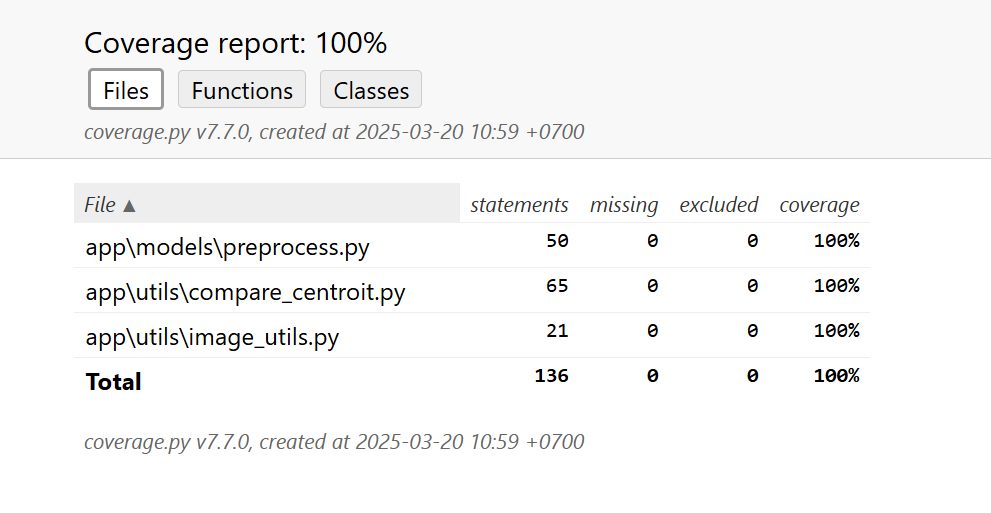
\includegraphics[width=1\textwidth]{figures/c4/4-3/pytest_2.png}
    \caption{Độ phủ kiểm thử xử lý logic với pytest.}
    \label{fig:pytest-testing}
\end{figure}


\subsubsection{Kiểm thử API}

Chi tiết các ca kiểm thử (miêu tả, input và output) được mô tả tại folder "[test]" tại đây\footnote{\url{http://bit.ly/42y7KyF}}. 
Và Hình \ref{fig:postman} dưới đây mô tả các API endpoint được kiểm thử với Postman\cite{postman}.  

\begin{figure}[H]
    \centering  
    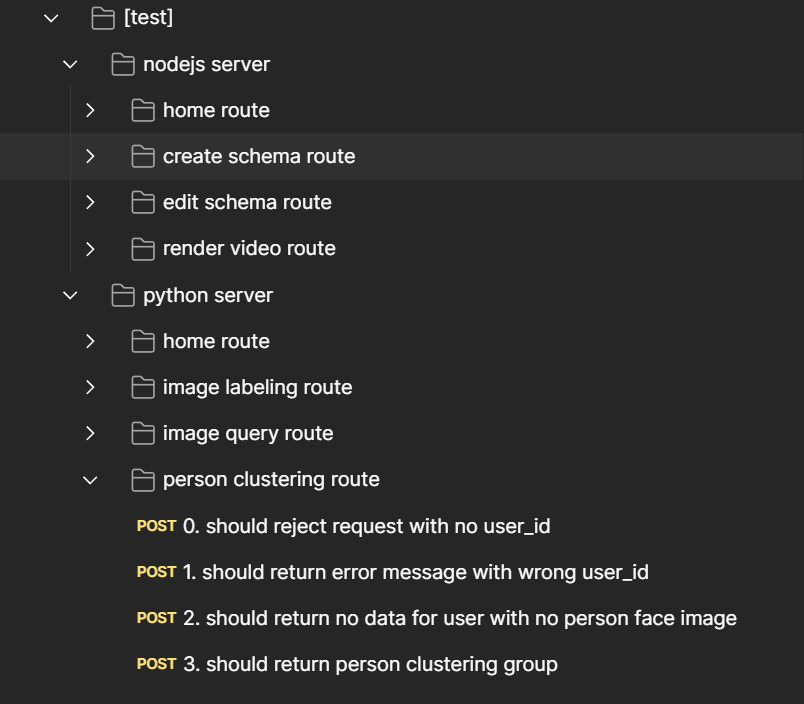
\includegraphics[width=0.7\textwidth]{figures/c4/4-3/api.png}
    \caption{Các API endpoint được kiểm thử với Postman.}
    \label{fig:postman}
\end{figure}


Bảng 4.1 dưới đây mô tả một số kịch bảng kiểm thử API chính cho ứng dụng. 

\small
\begin{xltabular}{\textwidth}{|c|p{2cm}|X|X|c|}
    \caption{Các kịch bản kiểm thử API chính} \label{tab:api-test-cases} \\
    \hline
    \textbf{STT} & \textbf{API} & \textbf{Ca kiểm thử} & \textbf{Kết quả kỳ vọng} & \textbf{Tình trạng} \\
    \hline
    \endfirsthead
    
    \multicolumn{5}{c}{\tablename\ \thetable{} (tiếp theo)} \\
    \hline
    \textbf{STT} & \textbf{API} & \textbf{Ca kiểm thử} & \textbf{Kết quả kỳ vọng} & \textbf{Tình trạng} \\
    \hline
    \endhead
    
    \hline \multicolumn{5}{r}{\textit{Tiếp trang sau}} \\
    \endfoot
    
    \hline
    \endlastfoot
    
    \multirow{3}{*}{1} & \multirow{3}{=}{\centering API tạo kịch bản video} & Tạo kịch bản video từ 5 hình ảnh hợp lệ & Hệ thống tạo được kịch bản, trả về mã 201 và thông tin kịch bản vừa tạo & Đạt \\
    \cline{3-5}
     & & Tạo kịch bản video không kèm theo ảnh & Hệ thống trả về mã lỗi 400 và thông báo cần gửi kèm danh sách ảnh & Đạt \\
    \cline{3-5}
    & & Người dùng chưa xác thực tạo kịch bản video & Hệ thống trả về mã lỗi 400 và thông báo cần xác thực & Đạt \\
    \hline
    \multirow{2}{*}{2} & \multirow{2}{=}{\centering API sửa kịch bản video} & Thay đổi tiêu đề video & Hệ thống thay đổi kịch bản, trả về mã 201 và thông tin kịch bản vừa được cập nhật & Đạt \\
    \cline{3-5}
     & & Thay đổi kịch bản video với params sai định dạng & Hệ thống trả về mã lỗi 400 và thông báo cần gửi yêu cầu đúng định dạng & Đạt \\
    \hline
    \multirow{3}{*}{3} & \multirow{3}{=}{\centering API tạo video} & Tạo video với kịch bản có sẵn & Hệ thống trả về ID của video cùng mã 201 & Đạt \\
    \cline{3-5}
     & & Tạo video không kèm theo token người dùng & Hệ thống trả về mã lỗi 400 và thông báo cần xác thực & Đạt \\
    \cline{3-5}
     & & Yêu cầu tạo cùng 1 video 2 lần & Hệ thống trả về mã lỗi 400 và thông báo lỗi video đang được tạo & Đạt \\
    \hline
    \multirow{2}{*}{4} & \multirow{2}{=}{\centering API tìm kiếm hình ảnh} & Tìm kiếm với từ khóa & Hệ thống trả về danh sách hình ảnh phù hợp và mã 200 & Đạt \\
    \cline{3-5}
     & & Người dùng chưa xác thực yêu cầu tìm kiếm với từ khóa & Hệ thống trả về mã lỗi 400 và thông báo cần xác thực & Đạt \\
    \hline
    \multirow{2}{*}{5} & \multirow{2}{=}{\centering API phân nhóm khuôn mặt} & Phân nhóm khuôn mặt với danh sách ảnh không có khuôn mặt & Hệ thống trả về danh sách rỗng và mã 200 & Đạt \\
    \cline{3-5}
     & & Phân nhóm khuôn mặt với danh sách 20 ảnh chứa 40 khuôn mặt & Hệ thống trả về danh sách nhóm khuôn mặt tương tự và mã 200 & Đạt \\
    \hline
    \multirow{3}{*}{6} & \multirow{3}{=}{\centering API gán nhãn ảnh} & Phân nhóm khuôn mặt với danh sách ảnh không có khuôn mặt & Hệ thống trả về danh sách rỗng và mã 200 & Đạt \\
    \cline{3-5}
     & & Gán nhãn 1 ảnh & Hệ thống trả nhãn của ảnh và mã 200 & Đạt \\
    \cline{3-5}
     & & Gán nhãn nhiều ảnh & Hệ thống trả về mảng nhãn ảnh và mã 200 & Đạt \\
    \hline
\end{xltabular}



\subsection{Kiểm thử tương tác người dùng trên giao diện ứng dụng}

Hệ thống triển khai kiểm thử tương tác người dùng trên giao diện với các ca kiểm thử tính năng chính của hệ thống được báo cáo lại trong bảng \ref{tab:ui-test-cases}.

\small
\begin{xltabular}{\textwidth}{|c|p{5cm}|X|c|}
    \caption{Các kịch bản kiểm thử tương tác người dùng} \label{tab:ui-test-cases} \\
    \hline
    \textbf{STT} & \textbf{Ca kiểm thử} & \textbf{Kết quả kỳ vọng} & \textbf{Tình trạng} \\
    \hline
    \endfirsthead
    
    \multicolumn{4}{c}{\tablename\ \thetable{} (tiếp theo)} \\
    \hline
    \textbf{STT} & \textbf{Ca kiểm thử} & \textbf{Kết quả kỳ vọng} & \textbf{Tình trạng} \\
    \hline
    \endhead
    
    \hline \multicolumn{4}{r}{\textit{Tiếp trang sau}} \\
    \endfoot
    
    \hline
    \endlastfoot
    
    1 & Đăng nhập với tài khoản hợp lệ & Người dùng được chuyển hướng đến màn hình chính và hiển thị thư viện ảnh & Đạt \\
    \hline
    2 & Đăng nhập với mật khẩu không chính xác & Hiển thị thông báo lỗi "Mật khẩu không chính xác" & Đạt \\
    \hline
    3 & Tải lên ảnh mới từ thiết bị & Ảnh được hiển thị trong thư viện và được phân loại tự động & Đạt \\
    \hline
    4 & Tìm kiếm ảnh bằng từ khóa & Hiển thị danh sách ảnh có liên quan đến từ khóa & Đạt \\
    \hline
    5 & Phân loại ảnh theo khuôn mặt & Hệ thống nhóm các ảnh có cùng khuôn mặt với độ chính xác trên 85\% & Đạt \\
    \hline
    6 & Tạo album mới và thêm ảnh vào & Album được tạo và hiển thị trong danh sách album với đúng số lượng ảnh & Đạt \\
    \hline
    7 & Tạo video recap từ ảnh trong album & Hệ thống tạo video và hiển thị trạng thái xử lý theo thời gian thực & Đạt \\
    \hline
    8 & Xem ảnh theo vị trí trên bản đồ & Bản đồ hiển thị các điểm đánh dấu ảnh theo đúng tọa độ GPS & Đạt \\
    \hline
    9 & Lọc ảnh theo ngày & Hiển thị chính xác những ảnh được chụp trong khoảng thời gian đã chọn & Đạt \\
    \hline
\end{xltabular}

\newpage\cleardoublepage
\chapter*{Kết luận}
\addcontentsline{toc}{chapter}{Kết luận}

Khóa luận này đã xây dựng được hệ thống quản lý thư viện ảnh tích hợp AI tạo video với đầy đủ các chức năng cơ bản như quản lý ảnh, phân loại tự động, tìm kiếm ảnh, và các tính năng nâng cao như tổ chức ảnh theo khuôn mặt, địa điểm, tạo album, và đặc biệt là tạo video recap từ bộ sưu tập ảnh với nhiều tùy chọn về chất lượng, chủ đề, nhạc nền, tiêu đề, v.v.

Bằng việc ứng dụng các mô hình AI như OpenCLIP và Face Recognition, hệ thống có khả năng tự động phân loại và gán nhãn ảnh, nhận diện khuôn mặt người, giúp người dùng quản lý bộ sưu tập hình ảnh của mình một cách thông minh và hiệu quả. Quy trình tạo video slideshow được xây dựng với nhiều thiết kế đa dạng cho phần Intro, Content và Outro, tích hợp thêm trí tuệ nhân tạo để tạo caption phù hợp cho từng video. Những tính năng này không chỉ giúp mang lại trải nghiệm độc đáo cho người dùng trong việc tạo ra những video recap ý nghĩa mà còn giúp họ tiết kiệm thời gian và công sức trong việc tìm kiếm và tổ chức ảnh.

Trong quá trình phát triển, do giới hạn của tài nguyên phần cứng, hệ thống AI và render video hiện chỉ được em chạy trên môi trường local. Đôi khi có sự cạnh tranh tài nguyên GPU giữa các service như phân loại khuôn mặt và gán nhãn ảnh, khiến chúng không thể chạy song song. Thời gian phân loại trung bình cho 300 gương mặt hiện đang là khoảng 10 giây, em sẽ cải thiện thêm về mặt hiệu suất và độ chính xác của thuật toán trong các phiên bản tiếp theo.\newpage\cleardoublepage

%\nocite{*}
\phantomsection 
\addcontentsline{toc}{chapter}{Tài liệu tham khảo}
\bibliography{references}\newpage\cleardoublepage
% \bibliographystyle{plain}
\end{document}


% NOTE: old tomtat.tex file

% \documentclass[a4paper,13pt]{report}
% \usepackage[utf8]{vietnam}
% \usepackage[utf8]{inputenc}
% \usepackage{amsmath}
% \usepackage{amsfonts}
% \usepackage{amssymb}
% \usepackage{graphicx}
% \usepackage{caption}
% \usepackage{booktabs}
% \usepackage[unicode]{hyperref}
% \usepackage[left=3cm,right=2cm,top=2.5cm,bottom=3cm]{geometry}
% \usepackage{titlesec} 
% \usepackage{scrextend}
% \usepackage{enumerate}
% \usepackage{tikz}
% \usepackage{float}
% \usepackage{sectsty}
% \usepackage{tocloft,calc}
% \usepackage{makecell}
% \usetikzlibrary{calc}

% \def\changemargin#1#2{\list{}{\rightmargin#2\leftmargin#1}\item[]}
% \let\endchangemargin=\endlist 

% \changefontsizes{13pt}

% \sectionfont{\fontsize{15}{15}\selectfont}
% \subsectionfont{\fontsize{13}{15}\selectfont}

% \titleformat{\chapter}[display]   
% {\normalfont\huge\bfseries}{\chaptertitlename\ \thechapter}{0pt}{\LARGE}
% \titlespacing*{\chapter}{0cm}{-\topskip}{0pt}[0pt]

% \renewcommand{\baselinestretch}{1.3}
% %\renewcommand{\cftsecpresnum}{Chương\space}
% \renewcommand{\cftchappresnum}{Chương }
% \AtBeginDocument{\addtolength\cftchapnumwidth{\widthof{\bfseries Chương }}}
% \setlength{\parskip}{0.4em}
% \setlength{\parindent}{0pt}
% %
% \title{Xây dựng ứng dụng quản lý nhóm chat sự kiện tích hợp AI tạo video}	%% title
% \author{Nguyễn Thành Dũng}			%% author's name

% %
% \newcommand{\argmax}{\arg\!\max}

% \begin{document}
% %% Cover Vietnamese 1

% Cover Vietnamese 1

\pagenumbering{gobble}
\begin{center}
	
\begin{tikzpicture}[overlay,remember picture]
	    \draw [line width=3pt,rounded corners=0pt,
	        ]
	        ($ (current page.north west) + (25mm,-25mm) $)
	        rectangle
	        ($ (current page.south east) + (-15mm,25mm) $);
	    \draw [line width=1pt,rounded corners=0pt]
	        ($ (current page.north west) + (26.5mm,-26.5mm) $)
	        rectangle
	        ($ (current page.south east) + (-16.5mm,26.5mm) $);
	\end{tikzpicture}
	\\[1mm]
	%%12pt
	\textbf{ĐẠI HỌC QUỐC GIA HÀ NỘI\\TRƯỜNG ĐẠI HỌC CÔNG NGHỆ}\\[1cm]
	
\includegraphics[width=0.2\linewidth]{figures/uet}\\[0.3cm]
	\textbf{Nguyễn Thành Dũng}
	\\[2cm]
	
	\large{\textbf{XÂY DỰNG ỨNG DỤNG QUẢN LÝ THƯ VIỆN ẢNH TÍCH HỢP AI TẠO VIDEO}}
	\\[2.6cm]
	\normalsize{\textbf{KHOÁ LUẬN TỐT NGHIỆP ĐẠI HỌC
		\\[2mm]
	Ngành: Công nghệ thông tin}}

	\vfill
	\textbf{HÀ NỘI - 2025}\vspace{10mm}
\end{center}

\begin{center}
	
	
\begin{tikzpicture}[overlay,remember picture]
	\draw [line width=3pt,rounded corners=0pt,
	]
	($ (current page.north west) + (25mm,-25mm) $)
	rectangle
	($ (current page.south east) + (-15mm,25mm) $);
	\draw [line width=1pt,rounded corners=0pt]
	($ (current page.north west) + (26.5mm,-26.5mm) $)
	rectangle
	($ (current page.south east) + (-16.5mm,26.5mm) $);
	\end{tikzpicture}
	\\[1mm]
	\textbf{ĐẠI HỌC QUỐC GIA HÀ NỘI\\TRƯỜNG ĐẠI HỌC CÔNG NGHỆ}
	\\[1cm]
	
\includegraphics[width=0.2\linewidth]{figures/uet}
	\\[0.3cm]
	\textbf{Nguyễn Thành Dũng}
	\\[2cm]
	
	\large{\textbf{XÂY DỰNG ỨNG DỤNG QUẢN LÝ THƯ VIỆN ẢNH TÍCH HỢP AI TẠO VIDEO}}
	\\[2.6cm]
	\normalsize{\textbf{KHOÁ LUẬN TỐT NGHIỆP ĐẠI HỌC
		\\[2mm]
	Ngành: Công nghệ thông tin}}
\end{center}
\vspace{16mm}
\hspace*{12mm}\textbf{ Cán bộ hướng dẫn: TS. Lê Khánh Trình}\\[0.8cm]
\hspace*{12mm}\textbf{ Cán bộ đồng hướng dẫn: TS. Đặng Trần Bình}
\vfill
\begin{center}
	\textbf{HÀ NỘI - 2025}\vspace{10mm}
\end{center}

% NOTE: Cover English 

% \begin{center}
	
% 	\begin{tikzpicture}[overlay,remember picture]
% 	\draw [line width=3pt,rounded corners=0pt,
% 	]
% 	($ (current page.north west) + (25mm,-25mm) $)
% 	rectangle
% 	($ (current page.south east) + (-15mm,25mm) $);
% 	\draw [line width=1pt,rounded corners=0pt]
% 	($ (current page.north west) + (26.5mm,-26.5mm) $)
% 	rectangle
% 	($ (current page.south east) + (-16.5mm,26.5mm) $);
% 	\end{tikzpicture}
% 	\\[1mm]
% 	\textbf{ VIETNAM NATIONAL UNIVERSITY, HANOI\\UNIVERSITY OF ENGINEERING AND TECHNOLOGY}
% 	\\[1cm]
% 	
\includegraphics[width=0.2\linewidth]{figures/uet}
% 	\\[0.3cm]
% 	\textbf{Nguyen Van A}
% 	\\[2cm]
	
% 	\textbf{THESIS TITLE}
% 	\\[2.6cm]
% 	\textbf{BACHELOR'S THESIS
% 		\\[2mm]
% 		Major: Information technology}
% \end{center}
% \vspace{16mm}
% \hspace*{12mm}\textbf{ Supervisor: Dr. ...}\\[0.8cm]
% \hspace*{12mm}\textbf{ Co-Supervisor: Dr. ...}
% \vfill
% \begin{center}
% 	\textbf{HANOI - 2022}
% 	\vspace{4mm}
% \end{center}

\newpage\cleardoublepage

% \pagenumbering{gobble}
% \begin{center}
	
% 	\begin{tikzpicture}[overlay,remember picture]
% 	\draw [line width=3pt,rounded corners=0pt,
% 	]
% 	($ (current page.north west) + (25mm,-25mm) $)
% 	rectangle
% 	($ (current page.south east) + (-15mm,25mm) $);
% 	\draw [line width=1pt,rounded corners=0pt]
% 	($ (current page.north west) + (26.5mm,-26.5mm) $)
% 	rectangle
% 	($ (current page.south east) + (-16.5mm,26.5mm) $);
% 	\end{tikzpicture}
% 	\\[1mm]
% 	\textbf{ĐẠI HỌC QUỐC GIA HÀ NỘI\\TRƯỜNG ĐẠI HỌC CÔNG NGHỆ}
% 	\\[1cm]
% 	
\includegraphics[width=0.2\linewidth]{figures/uet}
% 	\\[0.3cm]
% 	\textbf{Nguyễn Thành Dũng}
% 	\\[2cm]
	
% 	\textbf{XÂY DỰNG ỨNG DỤNG QUẢN LÝ NHÓM CHAT SỰ KIỆN TÍCH HỢP AI TẠO VIDEO}
% 	\\[2.6cm]
% 	\textbf{KHÓA LUẬN TỐT NGHIỆP ĐẠI HỌC HỆ CHÍNH QUY
% 		\\[2mm]
% 	Ngành: Công nghệ thông tin}
% \end{center}
% \vspace{16mm}
% \vfill
% \begin{center}
% 	\textbf{HÀ NỘI - 2025}\vspace{10mm}
% \end{center}

% \pagenumbering{gobble}
% \begin{center}
	
% 	\begin{tikzpicture}[overlay,remember picture]
% 	\draw [line width=3pt,rounded corners=0pt,
% 	]
% 	($ (current page.north west) + (25mm,-25mm) $)
% 	rectangle
% 	($ (current page.south east) + (-15mm,25mm) $);
% 	\draw [line width=1pt,rounded corners=0pt]
% 	($ (current page.north west) + (26.5mm,-26.5mm) $)
% 	rectangle
% 	($ (current page.south east) + (-16.5mm,26.5mm) $);
% 	\end{tikzpicture}
% 	\\[1mm]
% 	\textbf{ĐẠI HỌC QUỐC GIA HÀ NỘI\\TRƯỜNG ĐẠI HỌC CÔNG NGHỆ}
% 	\\[1cm]
% 	
\includegraphics[width=0.2\linewidth]{figures/uet}
% 	\\[0.3cm]
% 	\textbf{Nguyễn Thành Dũng}
% 	\\[2cm]
	
% 	\textbf{XÂY DỰNG ỨNG DỤNG QUẢN LÝ NHÓM CHAT SỰ KIỆN TÍCH HỢP AI TẠO VIDEO}
% 	\\[2.6cm]
% 	\textbf{KHÓA LUẬN TỐT NGHIỆP ĐẠI HỌC HỆ CHÍNH QUY
% 		\\[2mm]
% 		Major: Information Technology}
% \end{center}
% \vspace{16mm}
% \textbf{ Cán bộ hướng dân: TS. Lê Khánh Trình}
% \vfill
% \begin{center}
% 	\textbf{HÀ NỘI - 2025}\vspace{10mm}
% \end{center}
% \newpage\cleardoublepage

% \setcounter{page}{1}
% \pagenumbering{arabic}
% % Abstract Vietnamese
% \begin{center}
\textbf{\large{Tóm tắt}	}
\end{center}

\addcontentsline{toc}{chapter}{Tóm tắt}

\begin{small}
    Khóa luận tập trung xây dựng ứng dụng di động mang tên Smart Gallery nhằm hỗ trợ người dùng quản lý, tổ chức và tìm kiếm hình ảnh thông qua ứng dụng công nghệ trí tuệ nhân tạo. Smart Gallery cung cấp giao diện người dùng thân thiện, cho phép người dùng dễ dàng tương tác với kho ảnh cá nhân. Người dùng có thể xem và quản lý ảnh theo nhiều cách khác nhau như album, thời gian, tags, hoặc địa điểm.

    Một trong những điểm nổi bật của Smart Gallery là khả năng tự động phân loại và gắn nhãn ảnh theo các tiêu chí như địa điểm, hoạt động và sự kiện dựa trên nội dung hình ảnh. Hệ thống còn tích hợp công nghệ nhận diện khuôn mặt, cho phép người dùng quản lý và đặt tên cho các nhân vật xuất hiện trong ảnh, từ đó tạo điều kiện thuận lợi cho việc tìm kiếm và phân loại.
    
    Tính năng tìm kiếm thông minh của Smart Gallery cho phép người dùng tìm kiếm ảnh bằng văn bản hoặc giọng nói với nhiều tùy chọn lọc khác nhau như thời gian, album, nhân vật, v.v. Đặc biệt, ứng dụng còn hỗ trợ tạo video slideshow từ bộ sưu tập ảnh với khả năng tùy chỉnh đa dạng như theme, nhạc nền, độ phân giải và thời lượng.
    
    Ngoài ra, Smart Gallery còn cung cấp tính năng quản lý địa điểm cho ảnh và hiển thị vị trí các bức ảnh trên bản đồ, giúp người dùng dễ dàng theo dõi và có cái nhìn tổng quan về những nơi đã đến và địa điểm chụp ảnh.


\vspace*{1cm}
\textbf{Từ khóa}: 
\textit{Quản lý ảnh thông minh, Nhận diện khuôn mặt, Video slideshow recap, Smart Gallery.}
\end{small}\newpage\cleardoublepage
% % Abstract English
% \begin{center}
\textbf{\large{Abstract}	}
\end{center}

\addcontentsline{toc}{chapter}{Abstract}
\begin{small}



\vspace*{1cm}
\textbf{Keywords}: 
\end{small}\newpage\cleardoublepage

% \end{document}